% Options for packages loaded elsewhere
\PassOptionsToPackage{unicode}{hyperref}
\PassOptionsToPackage{hyphens}{url}
%
\documentclass[
  letterpaper,
]{scrbook}

\usepackage{amsmath,amssymb}
\usepackage{lmodern}
\usepackage{iftex}
\ifPDFTeX
  \usepackage[T1]{fontenc}
  \usepackage[utf8]{inputenc}
  \usepackage{textcomp} % provide euro and other symbols
\else % if luatex or xetex
  \usepackage{unicode-math}
  \defaultfontfeatures{Scale=MatchLowercase}
  \defaultfontfeatures[\rmfamily]{Ligatures=TeX,Scale=1}
\fi
% Use upquote if available, for straight quotes in verbatim environments
\IfFileExists{upquote.sty}{\usepackage{upquote}}{}
\IfFileExists{microtype.sty}{% use microtype if available
  \usepackage[]{microtype}
  \UseMicrotypeSet[protrusion]{basicmath} % disable protrusion for tt fonts
}{}
\makeatletter
\@ifundefined{KOMAClassName}{% if non-KOMA class
  \IfFileExists{parskip.sty}{%
    \usepackage{parskip}
  }{% else
    \setlength{\parindent}{0pt}
    \setlength{\parskip}{6pt plus 2pt minus 1pt}}
}{% if KOMA class
  \KOMAoptions{parskip=half}}
\makeatother
\usepackage{xcolor}
\setlength{\emergencystretch}{3em} % prevent overfull lines
\setcounter{secnumdepth}{5}
% Make \paragraph and \subparagraph free-standing
\ifx\paragraph\undefined\else
  \let\oldparagraph\paragraph
  \renewcommand{\paragraph}[1]{\oldparagraph{#1}\mbox{}}
\fi
\ifx\subparagraph\undefined\else
  \let\oldsubparagraph\subparagraph
  \renewcommand{\subparagraph}[1]{\oldsubparagraph{#1}\mbox{}}
\fi


\providecommand{\tightlist}{%
  \setlength{\itemsep}{0pt}\setlength{\parskip}{0pt}}\usepackage{longtable,booktabs,array}
\usepackage{calc} % for calculating minipage widths
% Correct order of tables after \paragraph or \subparagraph
\usepackage{etoolbox}
\makeatletter
\patchcmd\longtable{\par}{\if@noskipsec\mbox{}\fi\par}{}{}
\makeatother
% Allow footnotes in longtable head/foot
\IfFileExists{footnotehyper.sty}{\usepackage{footnotehyper}}{\usepackage{footnote}}
\makesavenoteenv{longtable}
\usepackage{graphicx}
\makeatletter
\def\maxwidth{\ifdim\Gin@nat@width>\linewidth\linewidth\else\Gin@nat@width\fi}
\def\maxheight{\ifdim\Gin@nat@height>\textheight\textheight\else\Gin@nat@height\fi}
\makeatother
% Scale images if necessary, so that they will not overflow the page
% margins by default, and it is still possible to overwrite the defaults
% using explicit options in \includegraphics[width, height, ...]{}
\setkeys{Gin}{width=\maxwidth,height=\maxheight,keepaspectratio}
% Set default figure placement to htbp
\makeatletter
\def\fps@figure{htbp}
\makeatother
\newlength{\cslhangindent}
\setlength{\cslhangindent}{1.5em}
\newlength{\csllabelwidth}
\setlength{\csllabelwidth}{3em}
\newlength{\cslentryspacingunit} % times entry-spacing
\setlength{\cslentryspacingunit}{\parskip}
\newenvironment{CSLReferences}[2] % #1 hanging-ident, #2 entry spacing
 {% don't indent paragraphs
  \setlength{\parindent}{0pt}
  % turn on hanging indent if param 1 is 1
  \ifodd #1
  \let\oldpar\par
  \def\par{\hangindent=\cslhangindent\oldpar}
  \fi
  % set entry spacing
  \setlength{\parskip}{#2\cslentryspacingunit}
 }%
 {}
\usepackage{calc}
\newcommand{\CSLBlock}[1]{#1\hfill\break}
\newcommand{\CSLLeftMargin}[1]{\parbox[t]{\csllabelwidth}{#1}}
\newcommand{\CSLRightInline}[1]{\parbox[t]{\linewidth - \csllabelwidth}{#1}\break}
\newcommand{\CSLIndent}[1]{\hspace{\cslhangindent}#1}

\usepackage{makeidx}
\makeindex
\makeatletter
\@ifpackageloaded{tcolorbox}{}{\usepackage[many]{tcolorbox}}
\@ifpackageloaded{fontawesome5}{}{\usepackage{fontawesome5}}
\definecolor{quarto-callout-color}{HTML}{909090}
\definecolor{quarto-callout-note-color}{HTML}{0758E5}
\definecolor{quarto-callout-important-color}{HTML}{CC1914}
\definecolor{quarto-callout-warning-color}{HTML}{EB9113}
\definecolor{quarto-callout-tip-color}{HTML}{00A047}
\definecolor{quarto-callout-caution-color}{HTML}{FC5300}
\definecolor{quarto-callout-color-frame}{HTML}{acacac}
\definecolor{quarto-callout-note-color-frame}{HTML}{4582ec}
\definecolor{quarto-callout-important-color-frame}{HTML}{d9534f}
\definecolor{quarto-callout-warning-color-frame}{HTML}{f0ad4e}
\definecolor{quarto-callout-tip-color-frame}{HTML}{02b875}
\definecolor{quarto-callout-caution-color-frame}{HTML}{fd7e14}
\makeatother
\makeatletter
\makeatother
\makeatletter
\@ifpackageloaded{bookmark}{}{\usepackage{bookmark}}
\makeatother
\makeatletter
\@ifpackageloaded{caption}{}{\usepackage{caption}}
\AtBeginDocument{%
\ifdefined\contentsname
  \renewcommand*\contentsname{Table of contents}
\else
  \newcommand\contentsname{Table of contents}
\fi
\ifdefined\listfigurename
  \renewcommand*\listfigurename{List of Figures}
\else
  \newcommand\listfigurename{List of Figures}
\fi
\ifdefined\listtablename
  \renewcommand*\listtablename{List of Tables}
\else
  \newcommand\listtablename{List of Tables}
\fi
\ifdefined\figurename
  \renewcommand*\figurename{Figure}
\else
  \newcommand\figurename{Figure}
\fi
\ifdefined\tablename
  \renewcommand*\tablename{Table}
\else
  \newcommand\tablename{Table}
\fi
}
\@ifpackageloaded{float}{}{\usepackage{float}}
\floatstyle{ruled}
\@ifundefined{c@chapter}{\newfloat{codelisting}{h}{lop}}{\newfloat{codelisting}{h}{lop}[chapter]}
\floatname{codelisting}{Listing}
\newcommand*\listoflistings{\listof{codelisting}{List of Listings}}
\makeatother
\makeatletter
\@ifpackageloaded{caption}{}{\usepackage{caption}}
\@ifpackageloaded{subcaption}{}{\usepackage{subcaption}}
\makeatother
\makeatletter
\@ifpackageloaded{tcolorbox}{}{\usepackage[many]{tcolorbox}}
\makeatother
\makeatletter
\@ifundefined{shadecolor}{\definecolor{shadecolor}{rgb}{.97, .97, .97}}
\makeatother
\makeatletter
\makeatother
\makeatletter
\@ifpackageloaded{fontawesome5}{}{\usepackage{fontawesome5}}
\makeatother
\ifLuaTeX
  \usepackage{selnolig}  % disable illegal ligatures
\fi
\IfFileExists{bookmark.sty}{\usepackage{bookmark}}{\usepackage{hyperref}}
\IfFileExists{xurl.sty}{\usepackage{xurl}}{} % add URL line breaks if available
\urlstyle{same} % disable monospaced font for URLs
\hypersetup{
  pdftitle={Spracherwerb},
  pdfauthor={Teodor Petrič},
  hidelinks,
  pdfcreator={LaTeX via pandoc}}

\title{Spracherwerb}
\usepackage{etoolbox}
\makeatletter
\providecommand{\subtitle}[1]{% add subtitle to \maketitle
  \apptocmd{\@title}{\par {\large #1 \par}}{}{}
}
\makeatother
\subtitle{Usvajanje jezikaLanguage Acquisition}
\author{Teodor Petrič}
\date{16.02.23}

\begin{document}
\frontmatter
\maketitle
\ifdefined\Shaded\renewenvironment{Shaded}{\begin{tcolorbox}[breakable, enhanced, sharp corners, borderline west={3pt}{0pt}{shadecolor}, frame hidden, boxrule=0pt, interior hidden]}{\end{tcolorbox}}\fi

\renewcommand*\contentsname{Table of contents}
{
\setcounter{tocdepth}{2}
\tableofcontents
}
\mainmatter
\bookmarksetup{startatroot}

\hypertarget{section}{%
\chapter*{.}\label{section}}
\addcontentsline{toc}{chapter}{.}

\markboth{.}{.}

\begin{figure}

{\centering 

\href{https://www.clipartmax.com/middle/m2i8K9m2b1d3A0d3_alphabet-song-cartoon-clip-art-babys-babble\%21-babys-first-sight-words-baby/}{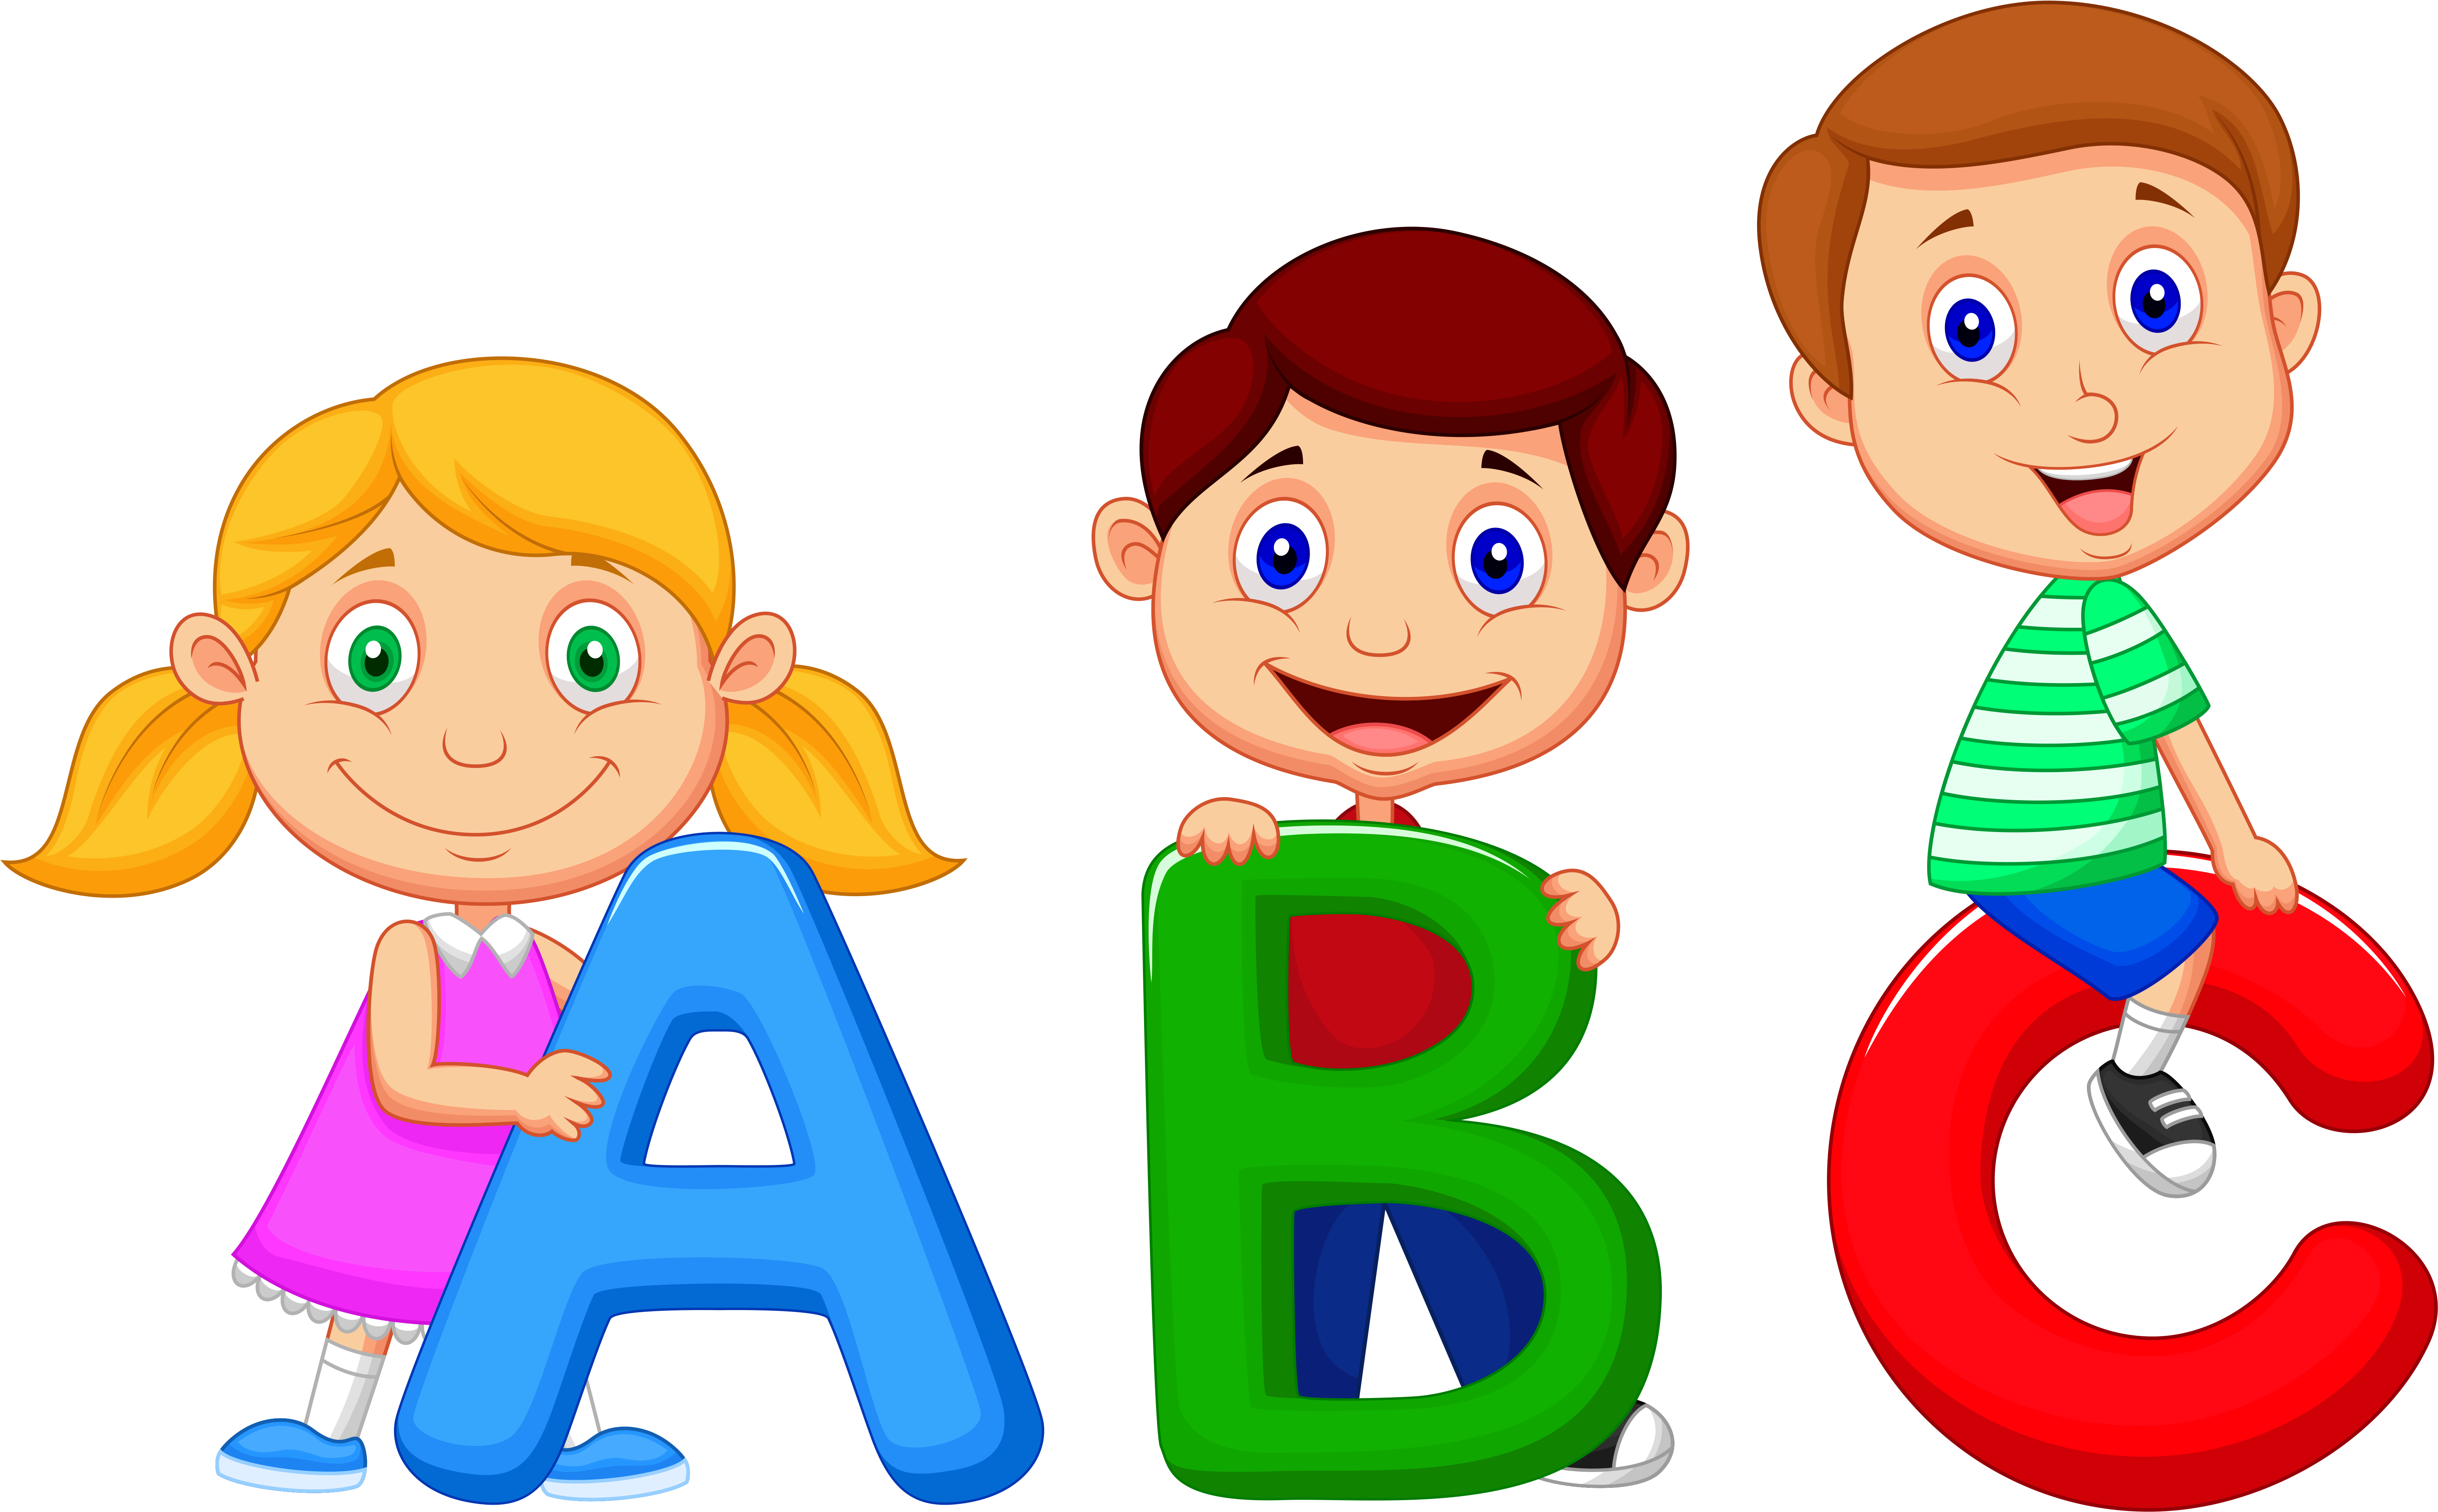
\includegraphics[width=1\textwidth,height=\textheight]{./pictures/clipart145720.png}}

}

\end{figure}

\bookmarksetup{startatroot}

\hypertarget{sec-vorwort}{%
\chapter*{Vorwort}\label{sec-vorwort}}
\addcontentsline{toc}{chapter}{Vorwort}

\markboth{Vorwort}{Vorwort}

Dieses Buch enthält Begleittexte und Übungsvorschläge für das
Studienfach \emph{Spracherwerb} (sl. \emph{Usvajanje jezika}, en.
\emph{Language acquisition}), das im Rahmen des Germanistikstudiums an
der Universität Maribor als Wahl- und Pflichtfach angeboten wird.

Das Buch wurde mit Hilfe der Programmierungssprache \texttt{R}
\url{https://www.r-project.org/} und der von \texttt{RStudio}
\url{https://www.rstudio.com/} entwickelten Skriptsprache
\texttt{Rmarkdown} \url{https://rmarkdown.rstudio.com/} auf der
Entwickler-Platform \texttt{Github} \url{https://github.com/} als
\texttt{Quarto\ Book} \url{https://quarto.org/} veröffentlicht.

\part{Grundlagen}

\hypertarget{sec-einfuhrung}{%
\chapter{Einführung}\label{sec-einfuhrung}}

In diesem Buch besprechen wir Entwicklungsabläufe, Tendenzen und
Paradigmen im Erst- und Zweit-/Fremdspracherwerb des Deutschen
(teilweise auch im Slowenischen), die im Rahmen verschiedener
Forschungsbereiche (Psycho- und Neurolinguistik, Spracherwerb,
Sprachvarietäten, \ldots) diskutiert werden und auch für germanistische
Studien von Interesse sein können. Die verwendeten Methoden und
praktischen Aufgaben sind zum Teil verallgemeinerbar und übertragbar auf
andere intellektuelle Arbeitsbereiche.\footnote{Dieses Buch wurde mit
  \texttt{Quarto} \url{https://quarto.org/docs/books/} zusammengestellt.}

Die vorgesehenen \emph{Themenbereiche}:\\

\begin{itemize}
\tightlist
\item
  Leitfragen in der Spracherwerbsforschung,\\
\item
  Merkmale verschiedenener Spracherwerbstypen,\\
\item
  Vor- und Nachteile der Mehrsprachigkeit,\\
\item
  Neurobiologische und kognitive Grundlagen des Spracherwerbs,\\
\item
  Markante Thesen einflussreicher Spracherwerbstheorien,\\
\item
  Spracherwerbsstadien am Beispiel deutscher Kinder,\\
\item
  Entwicklungsverläufe und Paradigmen am Beispiel deutscher
  Spracherwerbskorpora,\\
\item
  Sprachproduktion und -rezeption im Zweit-/Fremdspracherwerb,\\
\item
  Entwicklungsbedingte und transferbedingte sprachliche Konstruktionen
  im Zweit-/Fremdspracherwerb (v.a. am Beispiel slowenischer
  Lernender).\\
\end{itemize}

In diesem Einführungskurs machen wir Sie mit einigen der grundlegenden
Methoden zur Erfassung der linguistischen Merkmale in deutschen (und in
einigen Abschnitten auch mit slowenischen) Texten bekannt.

Hinweise\footnote{Clipart von \url{https://www.clipartmax.com/}}:

Das ist eine Definition (rmdnote).

Das ist ein Tip oder eine Info (rmdtip).

Das ist ein Arbeitsvorschlag (rmdrobot).

Das ist der RStudio Logotyp (rmdrstudio).

Das ist eine Warnung (rmdwarning).

Das ist eine Fehlermeldung (rmderror).

\hypertarget{sec-gegenstand}{%
\chapter{Leitfragen in der
Spracherwerbsforschung}\label{sec-gegenstand}}

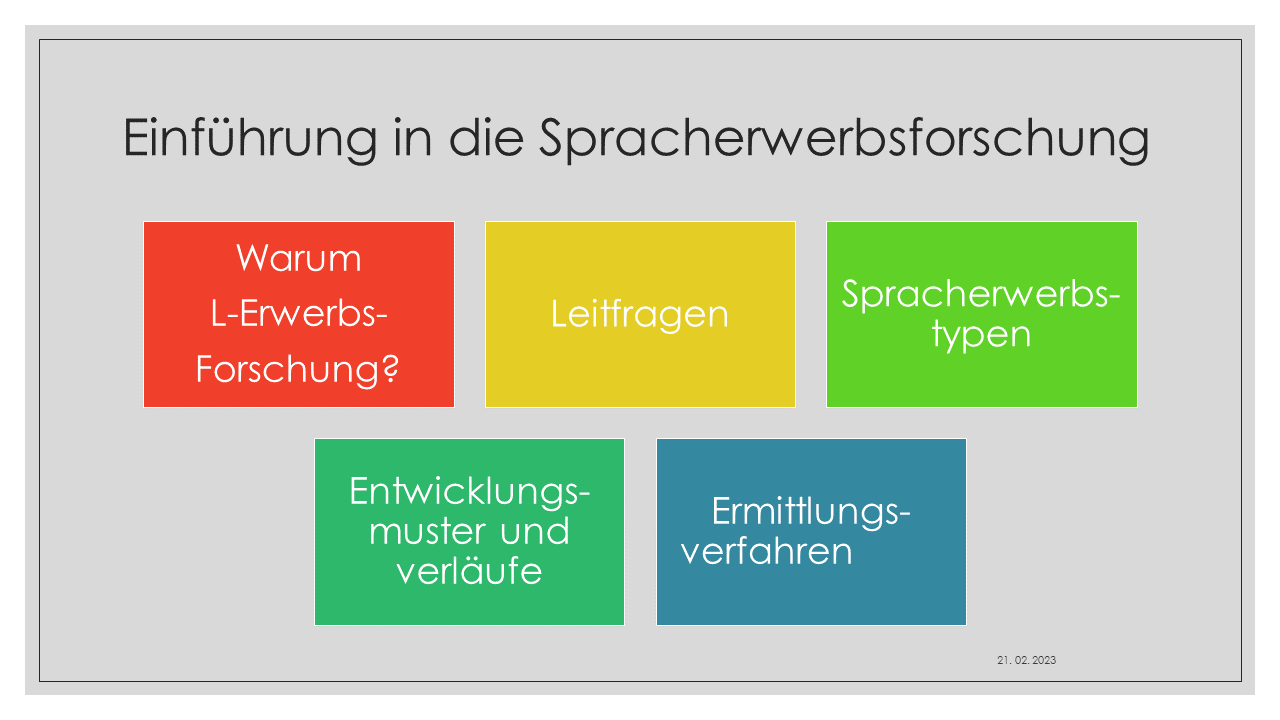
\includegraphics[width=1\textwidth,height=\textheight]{./pictures/UJ_Intro_2023_02.png}

Die Kernthemen der Spracherwerbsforschung lassen sich gemäß Kauschke
(2012) anhand von drei \textbf{Grundfragen} umreißen:

1. Was macht sprachliches Wissen, was macht die Beherrschung einer
Sprache aus?

2. Ist sprachliches Wissen angeboren oder wird es erlernt?

3. Wird Sprache über sprachspezifische oder über allgemein-kognitive
Mechanismen erworben?

\hypertarget{sprachbeherrschung}{%
\section{Sprachbeherrschung}\label{sprachbeherrschung}}

\textbf{Begriff des sprachlichen Wissens}

Sprache ist Bestandteil der menschlichen \textbf{Kognition}: Prozesse
der mentalen Speicherung, Aufnahme und Verarbeitung von Informationen.

Diesen Prozessen kann das \textbf{Bewusstsein} zugeschaltet sein oder
nicht.

Menge der gespeicherten Informationen (\textbf{deklaratives Wissen},
auch »Wissen, dass«)

Verfügbarkeit von informationsverarbeitenden Prozessen
(\textbf{prozedurales Wissen}, auch »Wissen, wie«).

Was macht nun sprachliches Wissen in diesem Sinne aus? Versteht man
Sprache als \textbf{gegliedertes System} von Einheiten, die durch ihre
Analysierbarkeit und ihre Kombinierbarkeit gekennzeichnet sind, so
bildet die \textbf{Entwicklung der Fähigkeit, sprachliche Einheiten zu
segmentieren und miteinander zu kombinieren, den Kern des
Spracherwerbs}.

Über den Aufbau sprachstrukturellen Wissens hinaus ist Wissen über die
\textbf{Gebrauchsbedingungen} von Sprache, ihre kommunikative Funktion
und ihren reziproken Charakter ebenfalls Gegenstand des Spracherwerbs.
Derartige anwendungsbezogene Aspekte von Sprache werden bereits
\textbf{im ersten Lebensjahr} in Austauschprozessen zwischen dem Kind
und seinen \textbf{Bezugspersonen} angebahnt und im weiteren Verlauf
ausdifferenziert.

\hypertarget{ist-sprachliches-wissen-angeboren-oder-wird-es-erlernt}{%
\section{Ist sprachliches Wissen angeboren oder wird es
erlernt?}\label{ist-sprachliches-wissen-angeboren-oder-wird-es-erlernt}}

Seit langem als Kernthema der Spracherwerbsforschung und immer wieder
neu diskutiert. Debatte um den Einfluss von Erbe und Umwelt auf die
Entwicklung von Individuen. Ausbildung dieser humanspezifischen
Fähigkeit nur möglich, wenn die sprachlernenden Menschen einer
Umgebungssprache ausgesetzt sind. Kontrovers wird diskutiert, welche
Rolle und welches Gewicht anlagebedingten Faktoren auf der einen Seite
und dem Sprachangebot der Umwelt auf der anderen Seite zukommt. Kommt
das Kind vorgeprägt für Sprache auf die Welt, ausgestattet mit
spezifischen Fähigkeiten, die in der menschlichen Entwicklungsgeschichte
entstanden sind? Entwickelt sich Sprache gemäß angeborener innerer
Voraussetzungen und vorgeprägter Reifungsprozesse entwickelt. Geht man
dagegen davon aus, dass das Kind Sprache aktiv und vorrangig durch
Kontakt und Kommunikation mit anderen Sprechern lernt.  

\hypertarget{domuxe4nenspezifik-von-sprache.}{%
\section{Domänenspezifik von
Sprache.}\label{domuxe4nenspezifik-von-sprache.}}

Wird Sprache über sprachspezifische oder allgemein-kognitive Mechanismen
erworben? Denkbar ist, dass allgemeine kognitive Prozesse auf
verschiedene Wissens- und Aufgabenbereiche anwendbar sind.

Eine andere Position besteht in der Annahme, dass für den Spracherwerb
domänenspezifisches Wissen notwendig ist, das darauf spezialisiert ist,
nur einen bestimmten Typus von Informationen zu verarbeiten.

In der Spracherwerbsforschung lassen sich drei große, traditionelle
Erklärungsparadigmen unterscheiden:

\begin{itemize}
\tightlist
\item
  Nativismus,
\item
  Interaktionismus und
\item
  Kognitivismus.
\end{itemize}

Neuere Erklärungsmodelle arbeiten auf eine Synthese hin.

\hypertarget{sec-zungenbrecher}{%
\chapter{Spracherwerbstypen}\label{sec-zungenbrecher}}

\begin{figure}

{\centering 

\href{https://www.clipartmax.com/middle/m2i8K9K9N4m2A0A0_fall-leaves-clip-art-september-writing/}{
\includegraphics[width=1\textwidth,height=\textheight]{./pictures/clipart49430.png}}

}

\end{figure}

\hypertarget{terminologische-unterscheidung}{%
\section{Terminologische
Unterscheidung}\label{terminologische-unterscheidung}}

In der Sprachewerbsforschung ist es möglich und üblich, verschiedene
Verben und Nomina zu verwenden, um auf verschiedene Spracherwerbstypen
Bezug zu nehmen.

\emph{Verben}: (eine Sprache) erwerben, sich (eine Sprache) aneignen,
(eine Sprache) lernen.

\emph{Nomina}: der Erwerb einer Sprache, die Aneignung einer Sprache,
das Lernen einer Sprache.

Welche semantischen Unterschiede bestehen zwischen den genannten Verben
und Nomina?

Vorschlag: Schauen Sie mal im \emph{DWDS} \url{https://www.dwds.de/}
nach und versuchen Sie festzustellen, in welchen Kontexten die Verben /
Nomina vorkommen!

Vergleichen Sie die Bedeutungen auch mit den Bedeutungen entsprechender
slowenischer und englischer Ausdrücke:

\emph{Slowenisch}: pridobiti (jezik), usvojiti (jezik), se učiti
(jezika).\\
\emph{Englisch}: acquire, learn (a language), \ldots{}

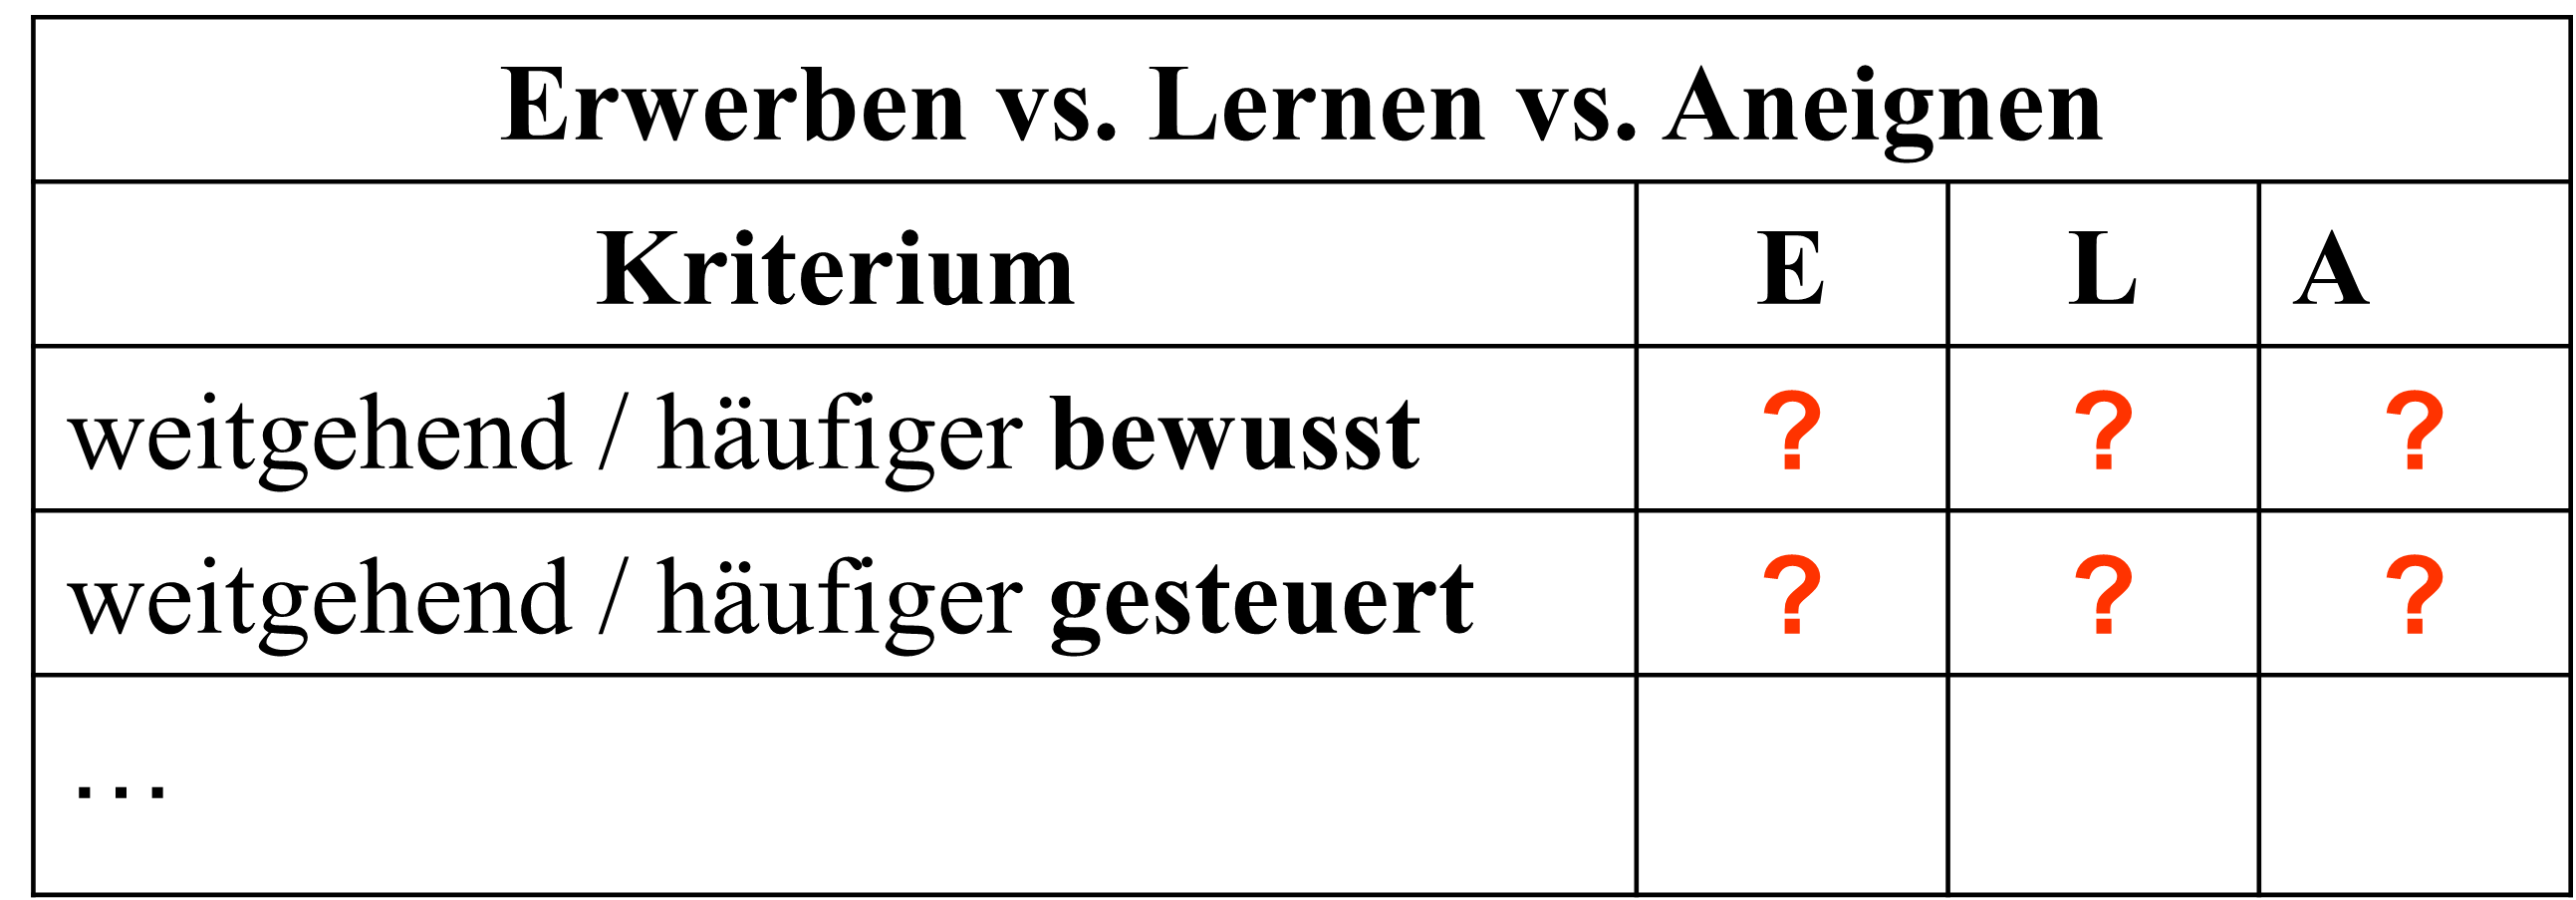
\includegraphics[width=8.62in,height=\textheight]{./pictures/termini_verben_nomen.png}

\emph{Aneignung} (A) soll als \emph{Oberbegriff} für Erwerb und Lernen
dienen. Die Aneignung einer Erstsprache ist stärker von
\emph{Erwerbsprozessen} geprägt. Die Aneignung einer Fremdsprache ist
stärker von \emph{Lernprozessen} geprägt. Die Aneignung einer
Zweitsprache (im engeren Sinne) ist je nach Fall stärker von
\emph{Erwerbs}- bzw. \emph{Lern}prozessen geprägt.

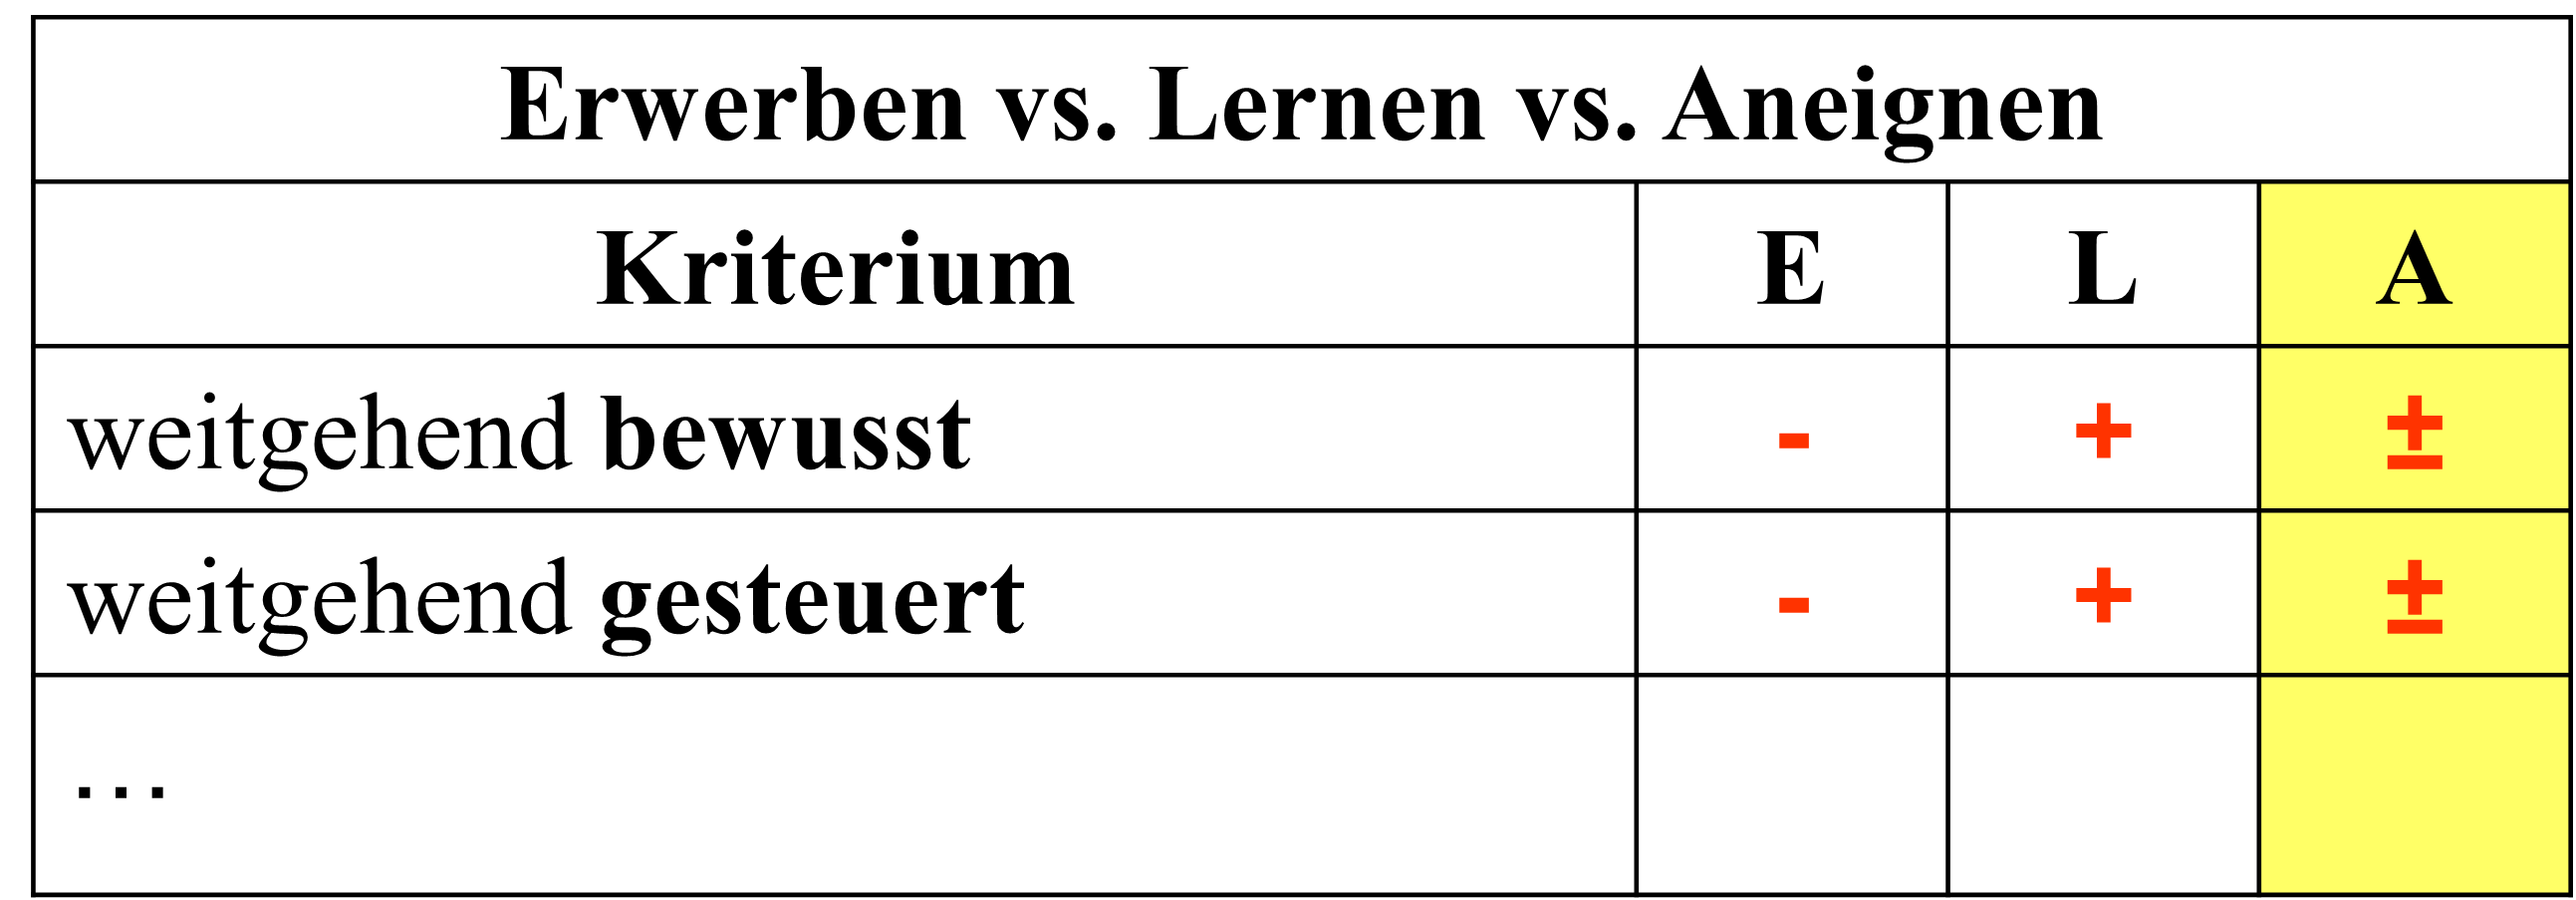
\includegraphics[width=8.62in,height=\textheight]{./pictures/termini_verben_nomen2.png}

Ihnen werden nun ein paar Videoausschnitte gezeigt, in denen die Art und
Weise beschrieben wird, wie sich Menschen eine Sprache aneignen.

Versuchen Sie, die wesentlichen Unterschiede und eventuelle
Gemeinsamkeiten herauszufinden !

\href{https://www.youtube.com/watch?v=cS_aH5wJGME}{Easy German} (Dauer:
11:07 Minuten):

\url{https://www.youtube.com/embed/cS_aH5wJGME}

\hypertarget{unterscheidungskriterien}{%
\section{Unterscheidungskriterien}\label{unterscheidungskriterien}}

Wir können eine Reihe von Kriterien verwenden, um drei
Spracherwerbstypen zu unterscheiden.

\emph{L1} steht für \emph{Erstsprache} (oft auch als
\emph{Muttersprache} bezeichnet), \emph{L2} bezieht sich auf die
\emph{Zweitsprache} und\\
\emph{FL} wird in der Tabelle für \emph{Fremdsprache} verwendet.

Der Ausdruck \emph{Muttersprache} ist bei bilingualen (d.h.
zweisprachigen) Personen nicht unbedingt zutreffend (\emph{warum?}),
darum ist \emph{Erstsprache} als Fachterminus zu bevorzugen.

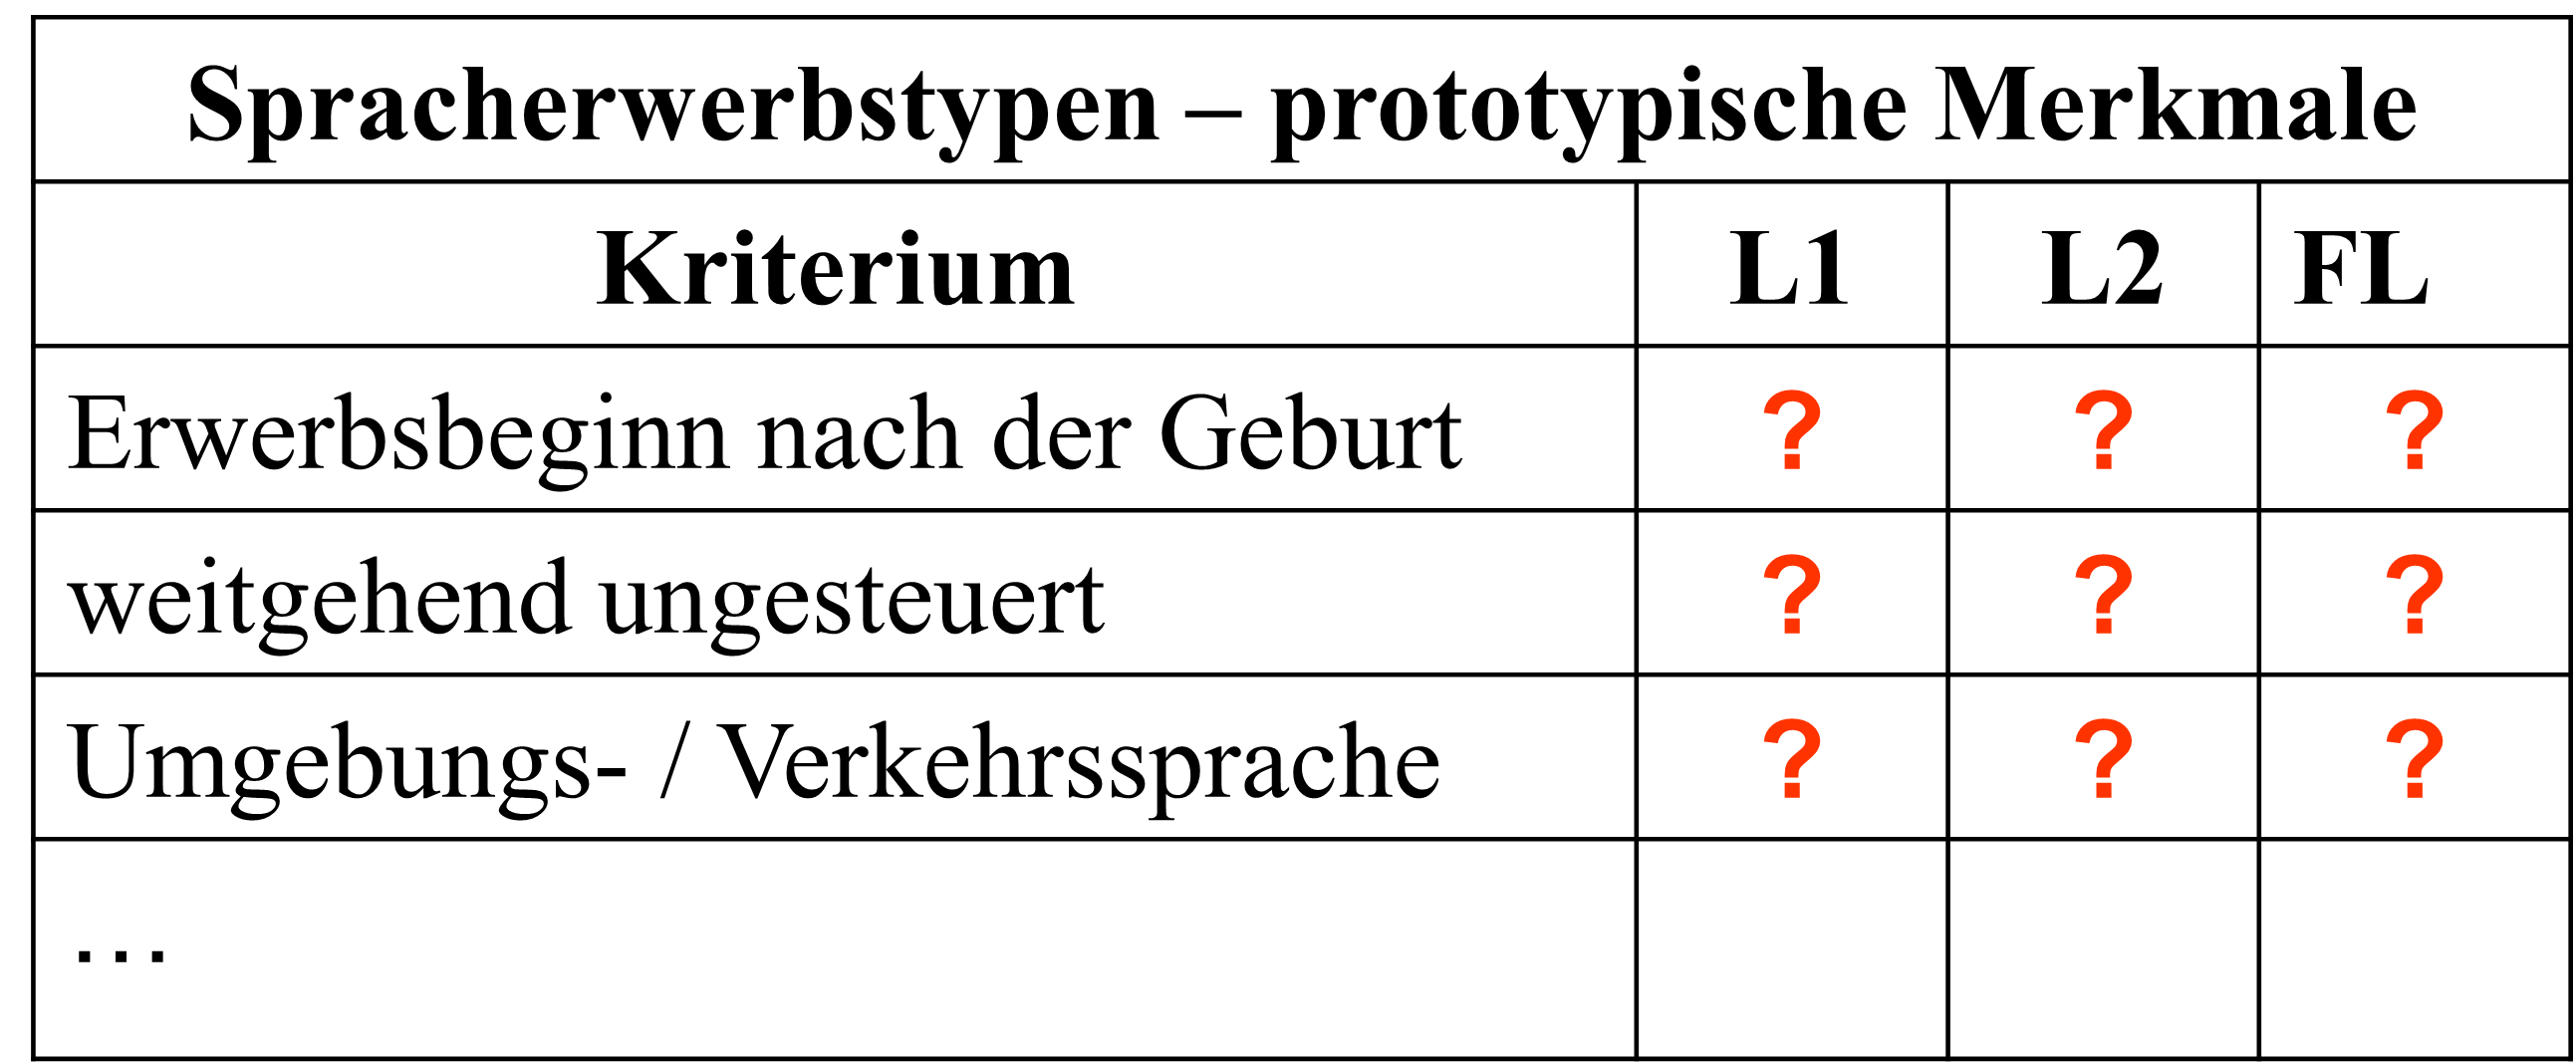
\includegraphics[width=8.62in,height=\textheight]{./pictures/spracherwerbstypen.png}

Ihnen werden nun ein paar Videoausschnitte gezeigt, in denen die Art und
Weise beschrieben wird, wie sich Menschen eine Sprache aneignen.

Versuchen Sie, die wesentlichen Unterschiede und eventuelle
Gemeinsamkeiten herauszufinden !

\href{https://www.youtube.com/watch?v=ZqObBG-NYPI}{Easy German} (Dauer:
8:46 Minuten):

\url{https://www.youtube.com/embed/ZqObBG-NYPI}

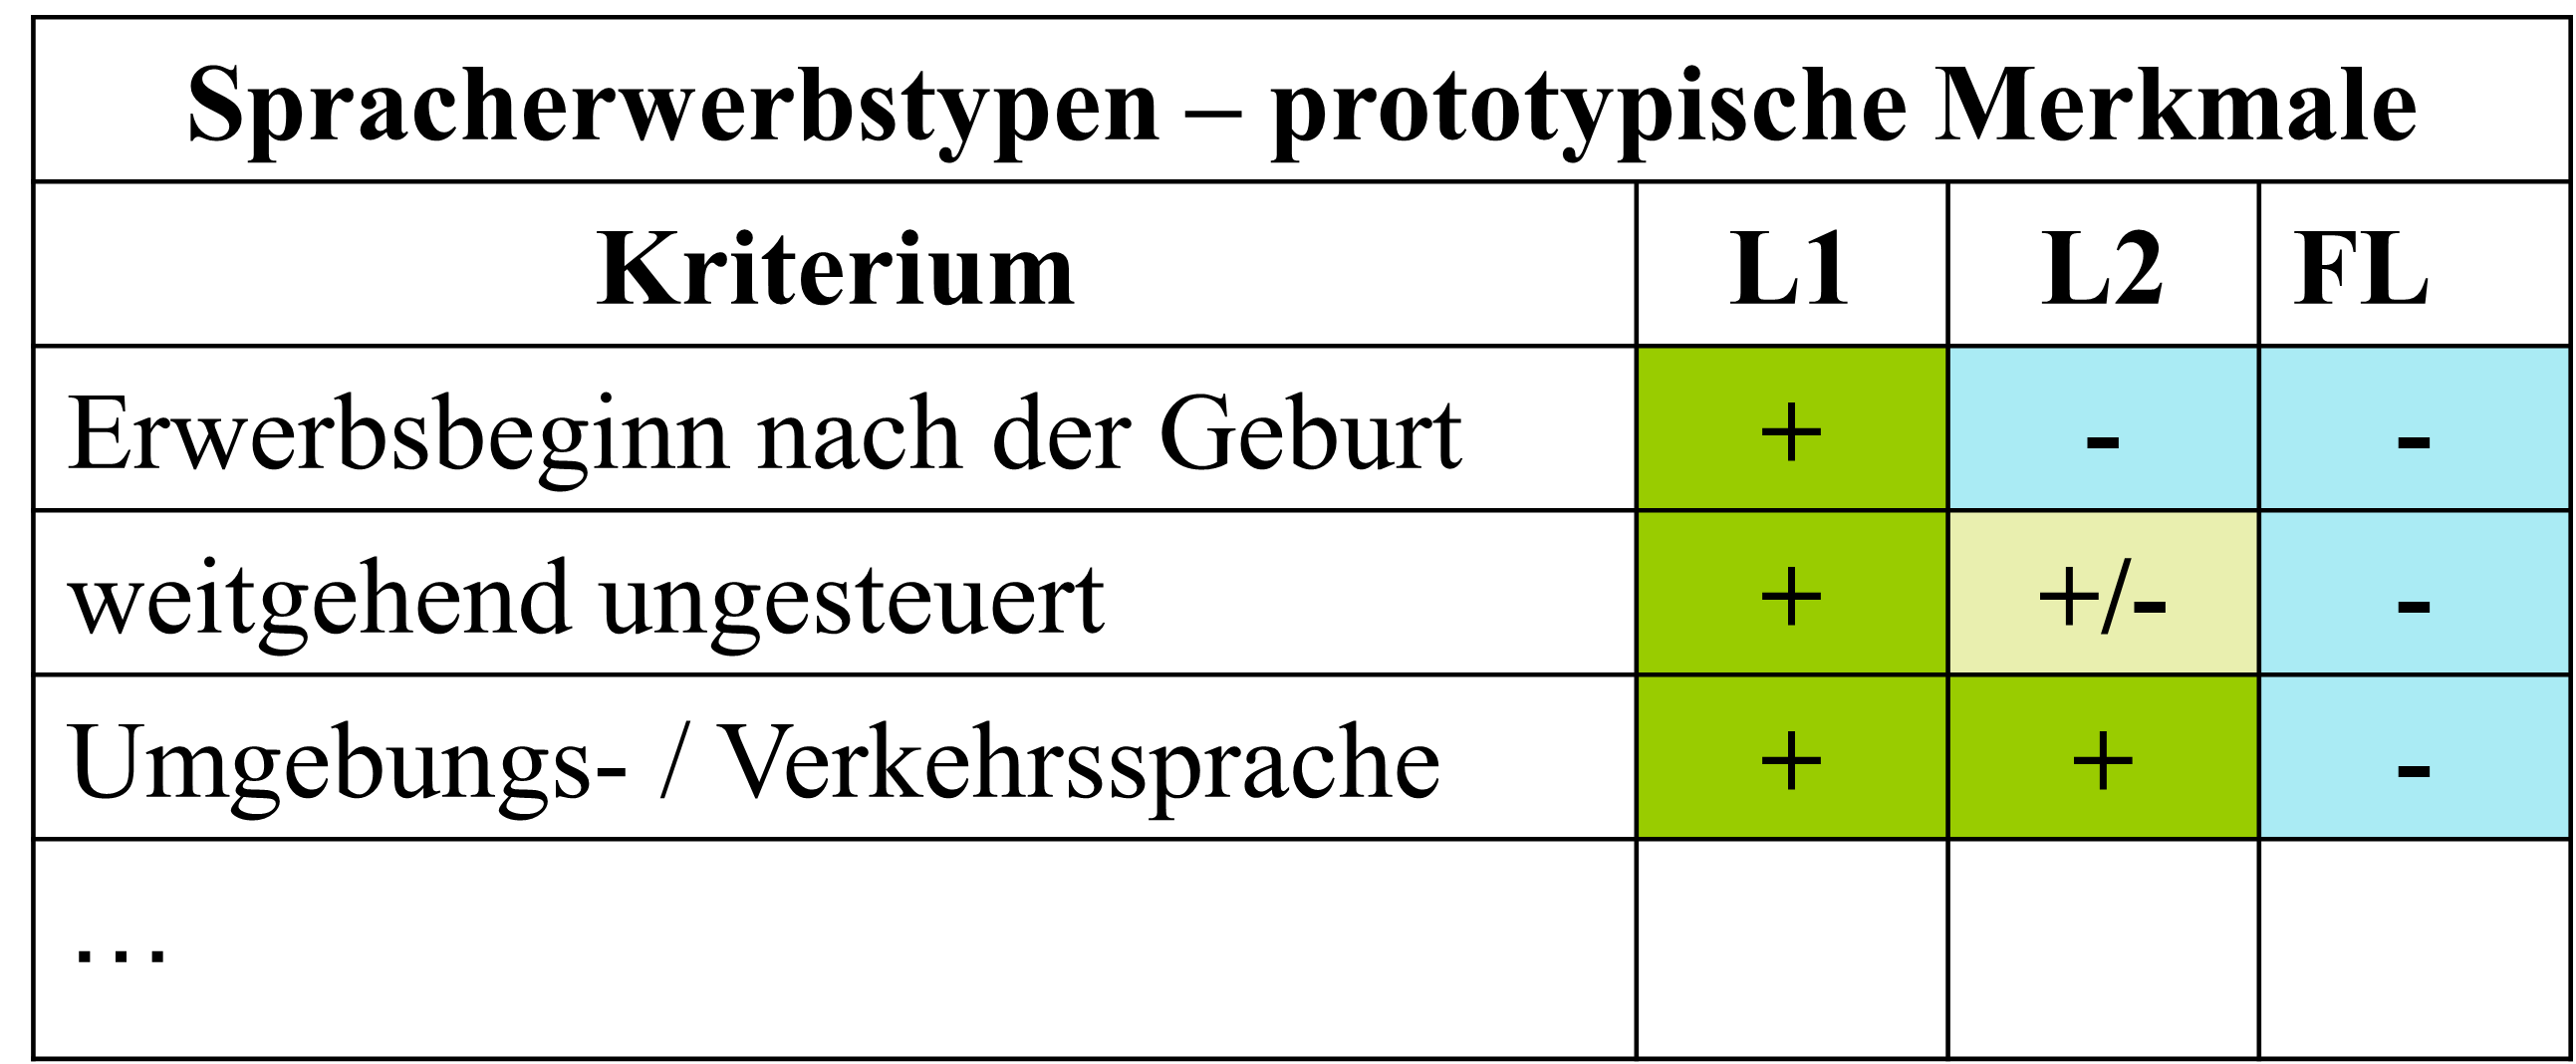
\includegraphics[width=8.62in,height=\textheight]{./pictures/spracherwerbstypen2.png}

In der Forschungsliteratur wird der Begriff \textbf{Zweitspracherwerb}

\begin{itemize}
\item
  \emph{im engeren Sinne} (wie in der zuvor gezeigten Tabelle),
\item
  bisweilen aber auch \emph{im weiteren Sinne} verwendet.
\end{itemize}

Im zweiten Fall werden Fremdspracherwerb und Zweitspracherwerb (im
engeren Sinne) als Zweitspracherwerb \textbf{zusammengefasst}. Welche
wichtige \textbf{Gemeinsamkeit} ist dafür wohl \textbf{ausschlaggebend}
?

Der Erstspracherwerb kann auch in der Form eines \textbf{doppelten
Erstspracherwerbs} (oder mehrfachen L1-Erwerbs) vorkommen.

Im Fall von bilingulaen Personen ist es auch aus neurobiologischer
Perspektive sinnvoll, zwischen \textbf{frühem} und \textbf{späten
Bilingualismus} zu unterscheiden.

\hypertarget{sec-bilingual}{%
\chapter{Vor- und Nachteile der Mehrsprachigkeit}\label{sec-bilingual}}

\begin{figure}

{\centering 

\href{https://www.clipartmax.com/middle/m2H7m2i8Z5A0N4Z5_lounge-style-sunglasses-retro-interlude-png-image-high-glasses-clipart-retro/}{
\includegraphics[width=1\textwidth,height=\textheight]{./pictures/clipart4776991.png}}

}

\end{figure}

Zwei- oder Mehrsprachigkeit hat nach Ansicht vieler Menschen mehrere
Vorteile. Aber viele Menschen wachsen nicht zwei- oder mehrsprachig auf.
Deshalb erhebt sich nicht nur die Frage, welche Vorteile
Mehrsprachigkeit hat, sondern auch, ob es gewisse Nachteile gibt, die
Mehrsprachigkeitsbestreben hemmen oder sogar verhindern.

Hier folgt eine Liste von Behauptungen zur Mehrsprachigkeit. Beurteilen
Sie, welche Behauptungen Sie für richtig halten und welche für nicht
haltbar.

\emph{Mobilitätsaspekte}:

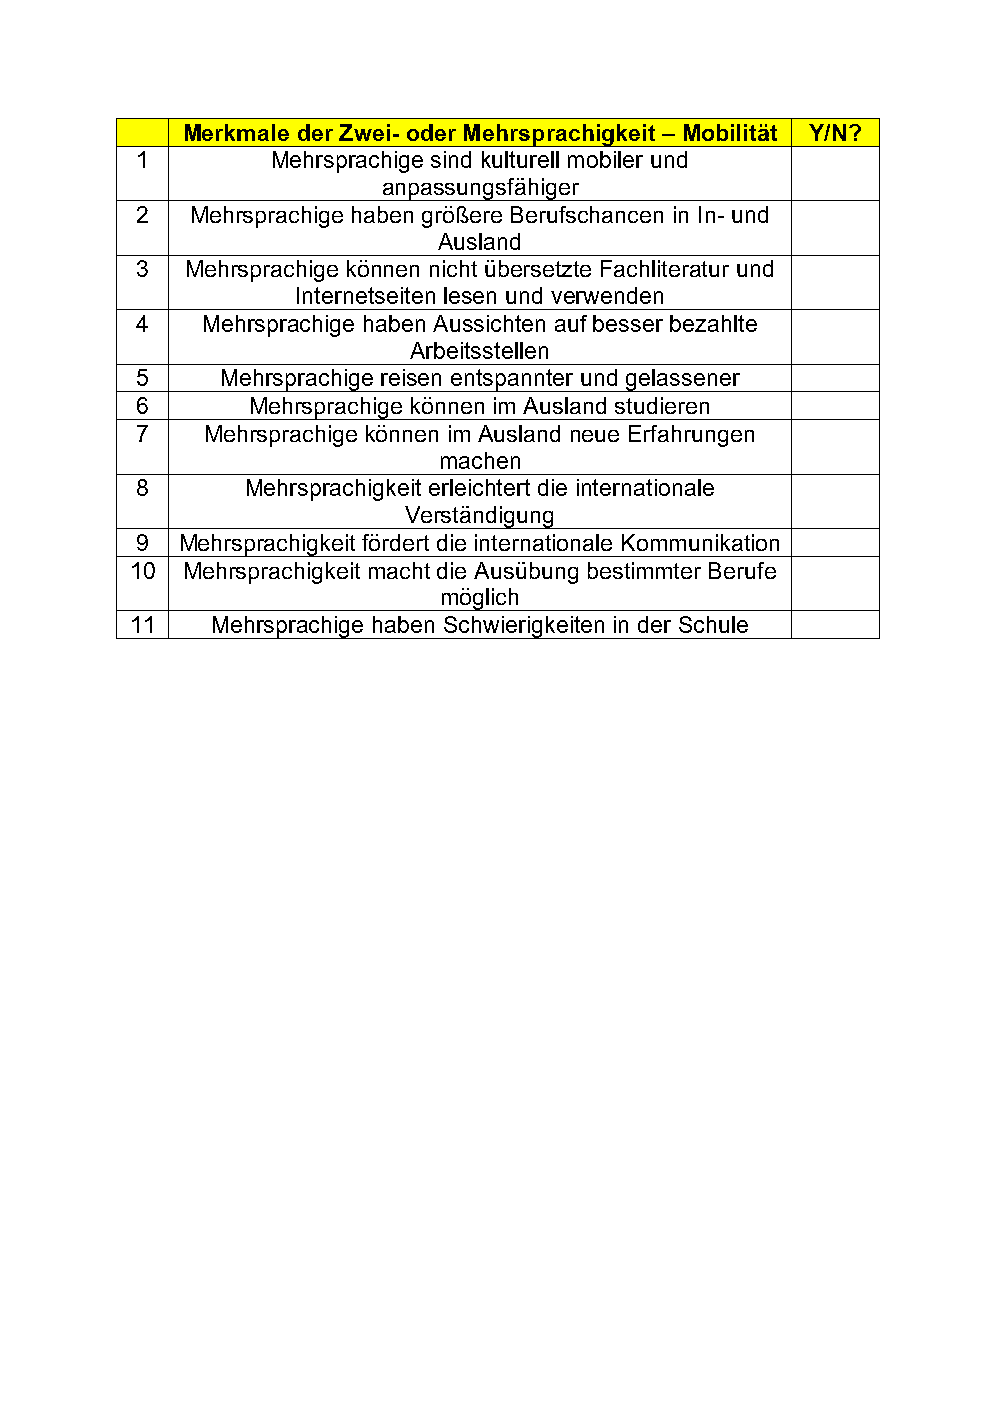
\includegraphics[width=3.31in,height=\textheight]{./pictures/Mehrsprachigkeit_Behauptungen_Page1.png}

\emph{Kulturelle Aspekte}:

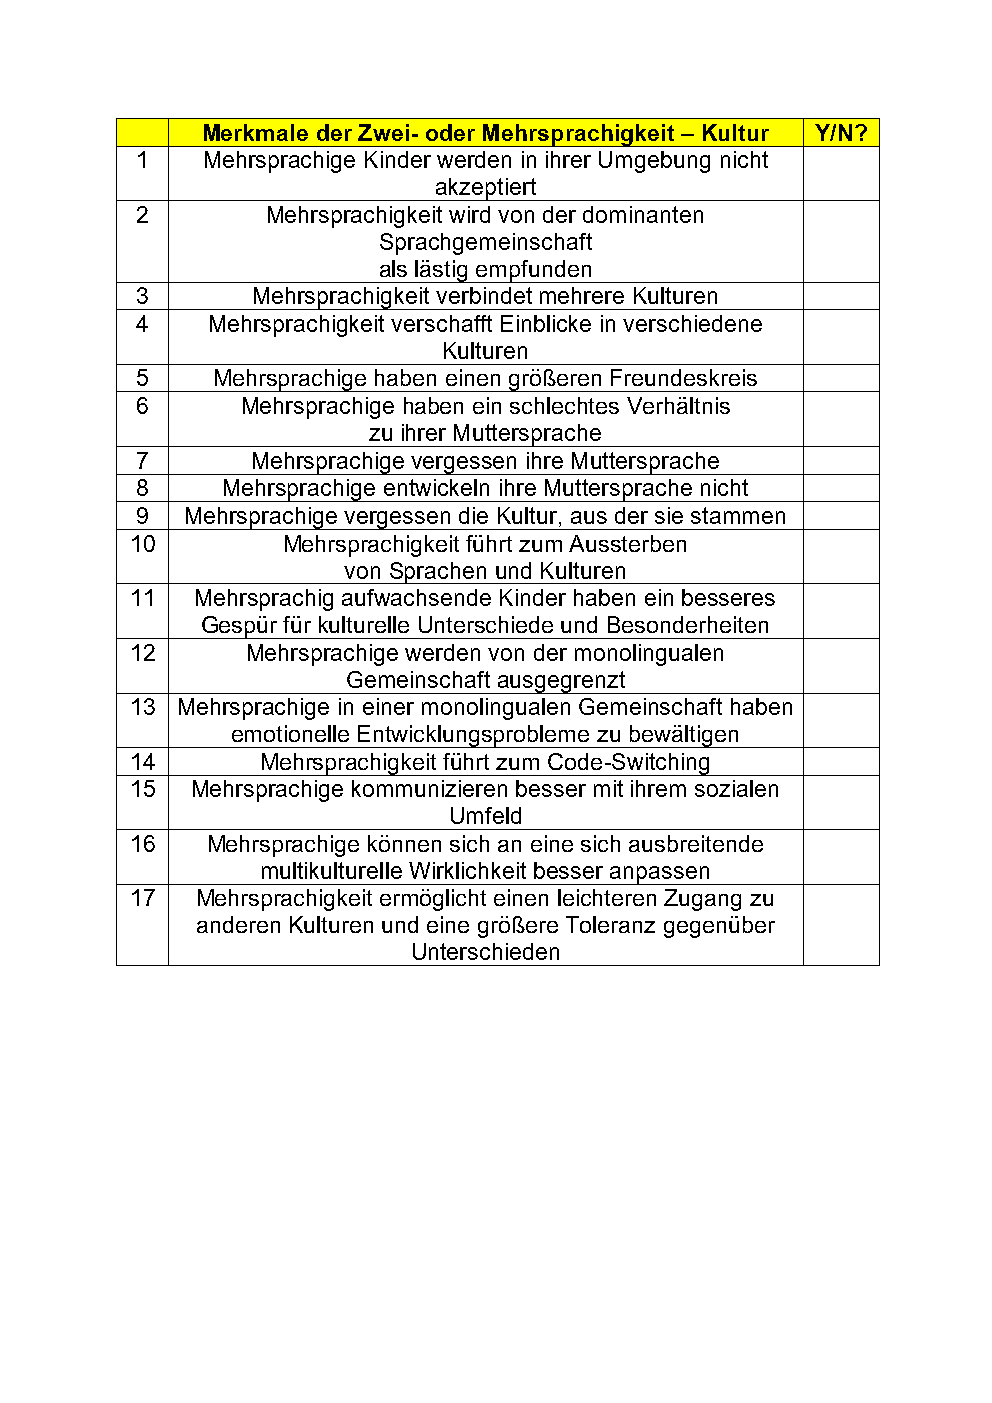
\includegraphics[width=3.31in,height=\textheight]{./pictures/Mehrsprachigkeit_Behauptungen_Page2.png}

\emph{Kognitive Aspekte}:

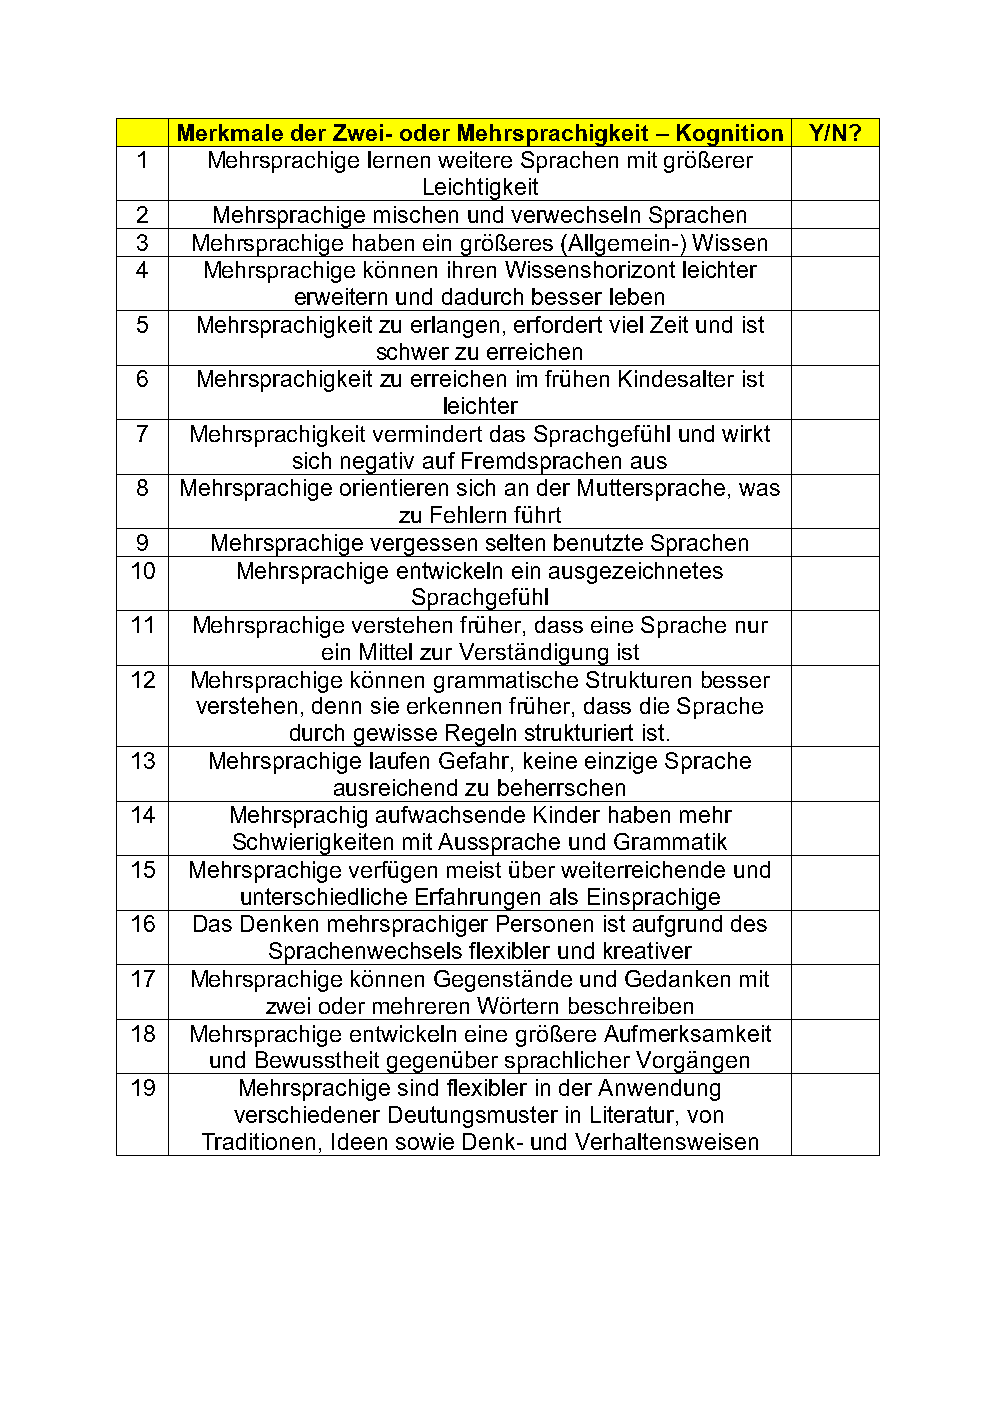
\includegraphics[width=3.31in,height=\textheight]{./pictures/Mehrsprachigkeit_Behauptungen_Page3.png}

In einem Artikel von \emph{Peter Ecke} Ecke (2008) werden \textbf{einige
Nachteile der Zwei- oder Mehrsprachigkeit} anhand von wissenschaftlichen
Studien diskutiert. Die Web-Adresse des Artikels:
\href{http://www.u.arizona.edu/~eckep/Ecke\%2008\%20Kosten\%20der\%20MS.pdf}{University
of Arizona}. Hier ist ein Abdruck der ersten Seite:

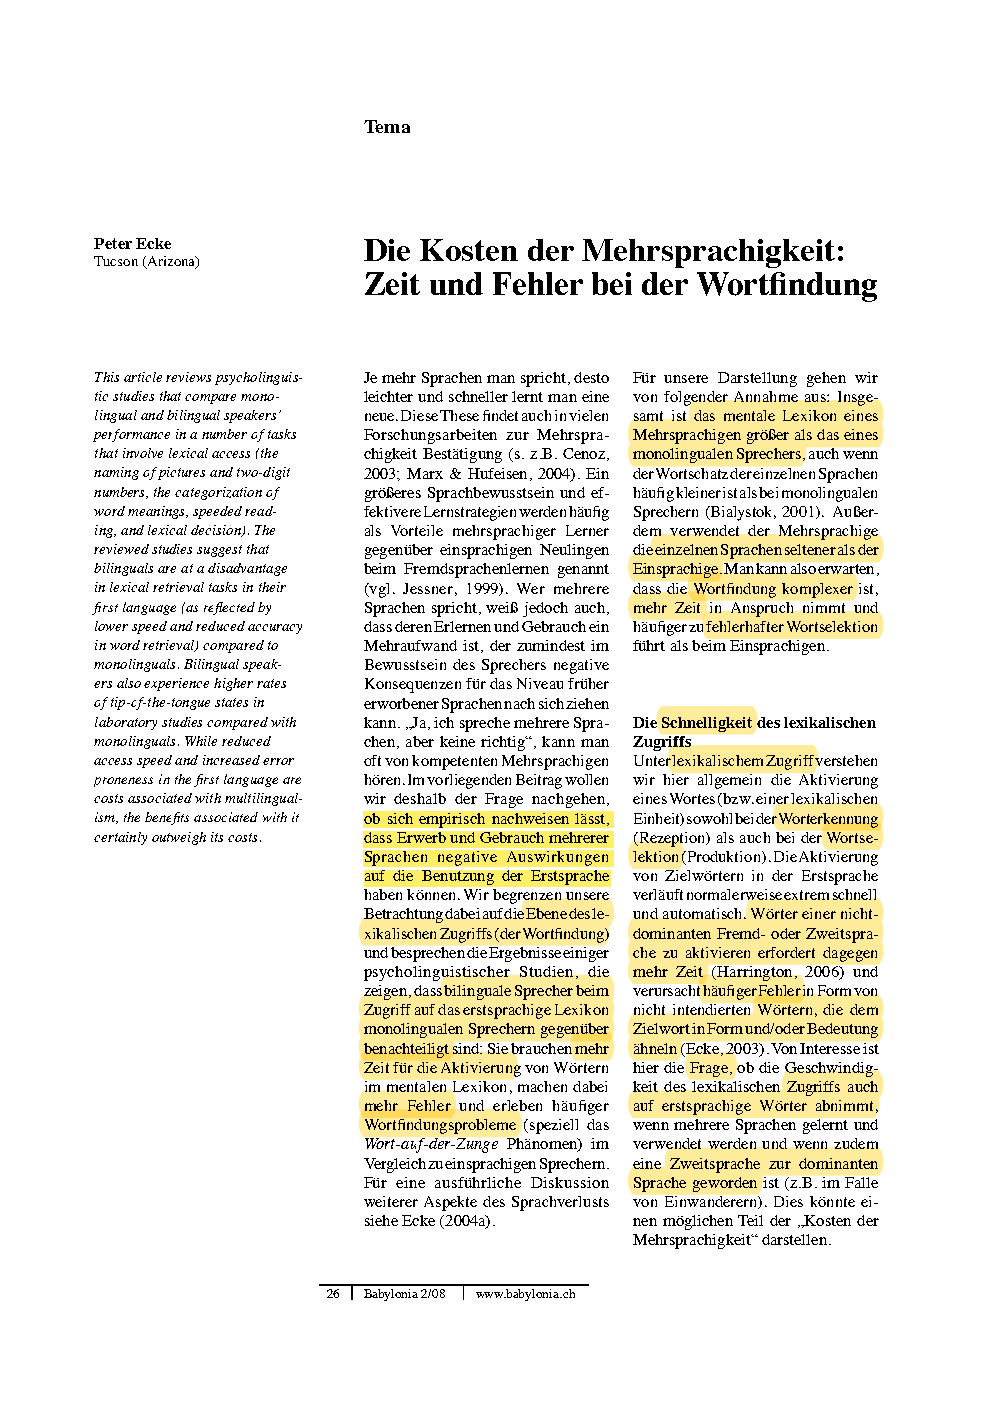
\includegraphics[width=3.31in,height=\textheight]{./pictures/TOT_bilangual_baby2_08ecke_annotated_Page1.png}

Ihnen werden nun Videos gezeigt, in denen Vorteile der
Zwei-/Mehrsprachigkeit und (vermeintliche) Nachteile erläutern werden.

Stellen Sie eine Liste der Vor- und Nachteile zusammen, damit Sie über
das Thema Mehrsprachigkeit diskutieren und entsprechend argumentieren
könen!

\href{https://www.youtube.com/watch?v=35XkRMBT28c}{Herzenssprache}
(Dauer: 7:53 Minuten):

\url{https://www.youtube.com/embed/35XkRMBT28c}

Ein weiteres Video zum Thema \emph{Mehrsprachigkeit}.

Stellen Sie eine Liste der Vor- und Nachteile zusammen, damit Sie über
das Thema Mehrsprachigkeit diskutieren und entsprechend argumentieren
könen!

\href{https://www.youtube.com/watch?v=0lJKipFitnA}{Wanderlust Monica}
(Dauer: 12:34 Minuten):

\url{https://www.youtube.com/embed/0lJKipFitnA}

Ein längeres Gespräch mit \emph{Prof.~Dr.~Jürgen Meisel} zum Thema
\emph{Mehrsprachigkeit}.

Stellen Sie eine Liste der Vor- und Nachteile zusammen, damit Sie über
das Thema Mehrsprachigkeit diskutieren und entsprechend argumentieren
könen!

\href{https://www.youtube.com/watch?v=a2Iw0jDkwYI}{Gabriel Gelman
Sprachheld} (Dauer: 43:53 Minuten):

\url{https://www.youtube.com/embed/a2Iw0jDkwYI}

Ein kürzeres Gespräch mit \emph{Prof.~Dr.~Rosemarie Tracy} über das
Thema \emph{Mehrsprachigkeit}.

Stellen Sie eine Liste der Vor- und Nachteile zusammen, damit Sie über
das Thema Mehrsprachigkeit diskutieren und entsprechend argumentieren
könen!

\href{https://www.youtube.com/watch?v=SAlTrh_76p0}{Universität Mannheim}
(Dauer: 10:51 Minuten):

\url{https://www.youtube.com/embed/SAlTrh_76p0}

Ein Vortrag von \emph{Prof.~Dr.~Rosemarie Tracy} über das Thema
\emph{Mehrsprachigkeit}.

\href{https://www.youtube.com/watch?v=vTK5-HSjbjs}{BildungsTV} (Dauer:
53:15 Minuten):

\url{https://www.youtube.com/embed/vTK5-HSjbjs}

Ein Vortrag von \emph{Prof.~Dr.~Rosemarie Tracy} über das Thema
\emph{Spracherwerb}.

\href{https://www.youtube.com/watch?v=prCbpoi-3KI}{BildungsTV} (Dauer:
1:04:48):

\url{https://www.youtube.com/embed/prCbpoi-3KI}

\hypertarget{sec-spracherwerb}{%
\chapter{Methoden in der
Spracherwerbsforschung}\label{sec-spracherwerb}}

\begin{figure}

{\centering 

\href{https://www.clipartmax.com/middle/m2i8K9i8K9m2i8A0_solutions-for-reducing-leadership-burnout-technology-doesn-t-work/}{
\includegraphics[width=1\textwidth,height=\textheight]{./pictures/clipart55029.png}}

}

\end{figure}

In jeder wissenschaftlichen Disziplin müssen Daten erhoben werden, um
Erklärungsansätze empirisch überprüfen zu können. Zu diesem Zweck werden
verschiedene Methoden eingesetzt, einen theoretischen Ansatz zu
falsifizieren. In Kauschke (2012): 6-22 werden verschiedene Verfahren
für die Gewinnung von Daten beschrieben, die in Untersuchungen zum
Erstspracherwerb eingesetzt werden. Viele davon finden jedoch auch in
Untersuchungen zum Zweit- und Fremdspracherwerb Anwendung.

Welche Methoden werden in Kauschke (2012) beschrieben?\\
Welche Anwendungsbereiche finden sie?\\
Welche Vor- und Nachteile zeigen sich bei ihrer Anwendung?

Stellen Sie eine Präsentation zum Thema zusammen und illustrieren Sie
sie auch mit Abbildungen und Beispielen, die Sie im Internet ausfindig
gemacht haben!

\begin{figure}

{\centering 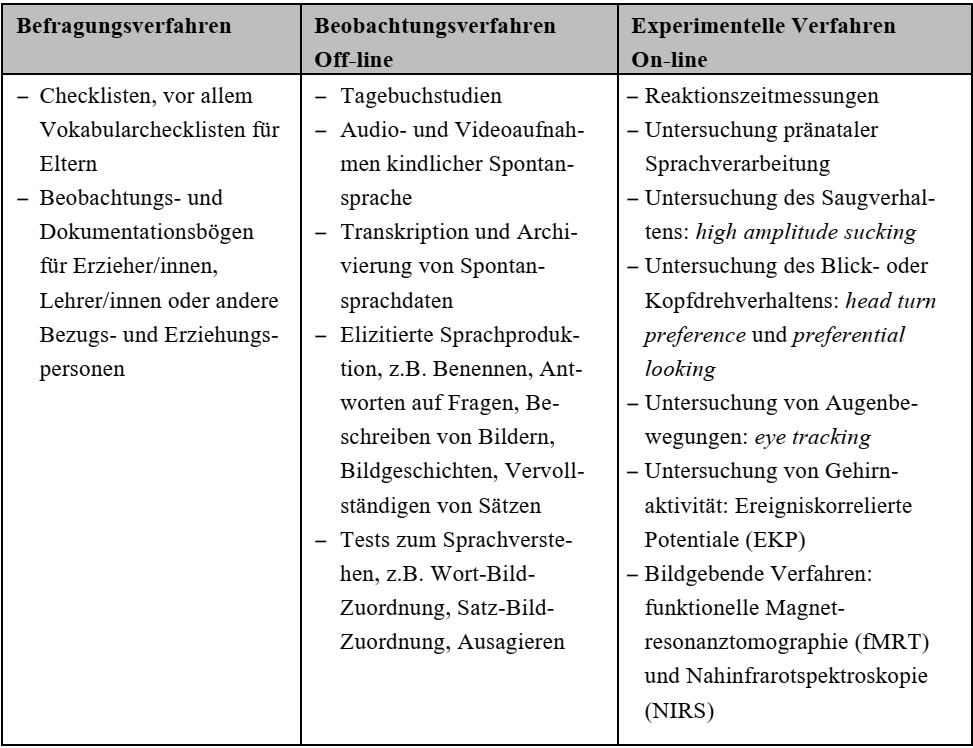
\includegraphics[width=1\textwidth,height=\textheight]{./pictures/methoden.png}

}

\caption{Übersicht über Methoden der Spracherwerbsforschung in Kauschke
(2012): 6}

\end{figure}

\hypertarget{sec-neuro}{%
\chapter{Neurobiologische und kognitive Grundlagen des
Spracherwerbs}\label{sec-neuro}}

\begin{figure}

{\centering 

\href{https://www.kissclipart.com/tongue-twister-cartoon-comics-stop-consonant-m2n92r/}{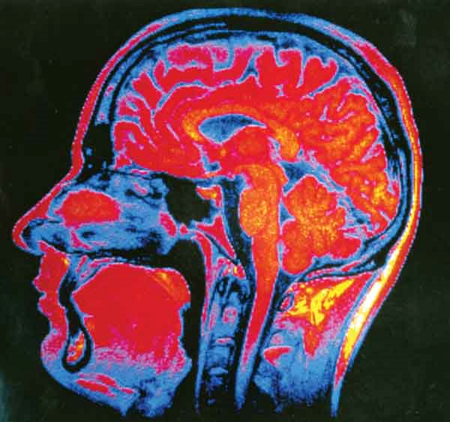
\includegraphics[width=1\textwidth,height=\textheight]{./pictures/brain_scan.png}}

}

\end{figure}

\hypertarget{hirnmasse}{%
\section{Hirnmasse}\label{hirnmasse}}

Das Gehirn eines Menschen ist vergleichsweise klein.

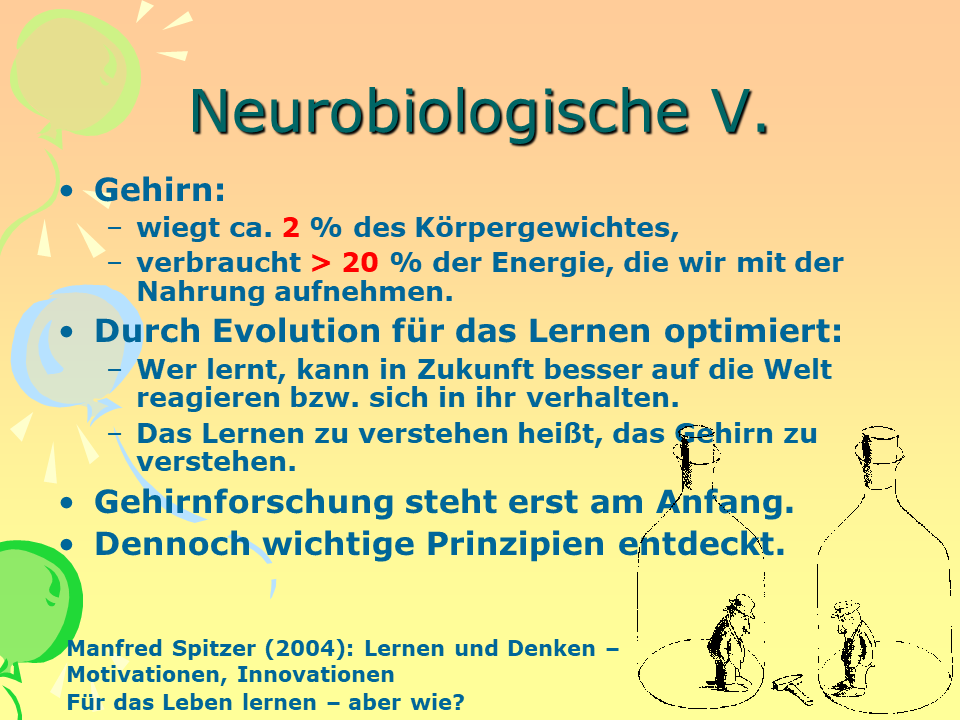
\includegraphics[width=1\textwidth,height=\textheight]{./pictures/neuro/Diapozitiv9.PNG}

Wie viel Hirnmasse hat der Mensch im Vergleich zu anderen Tieren?

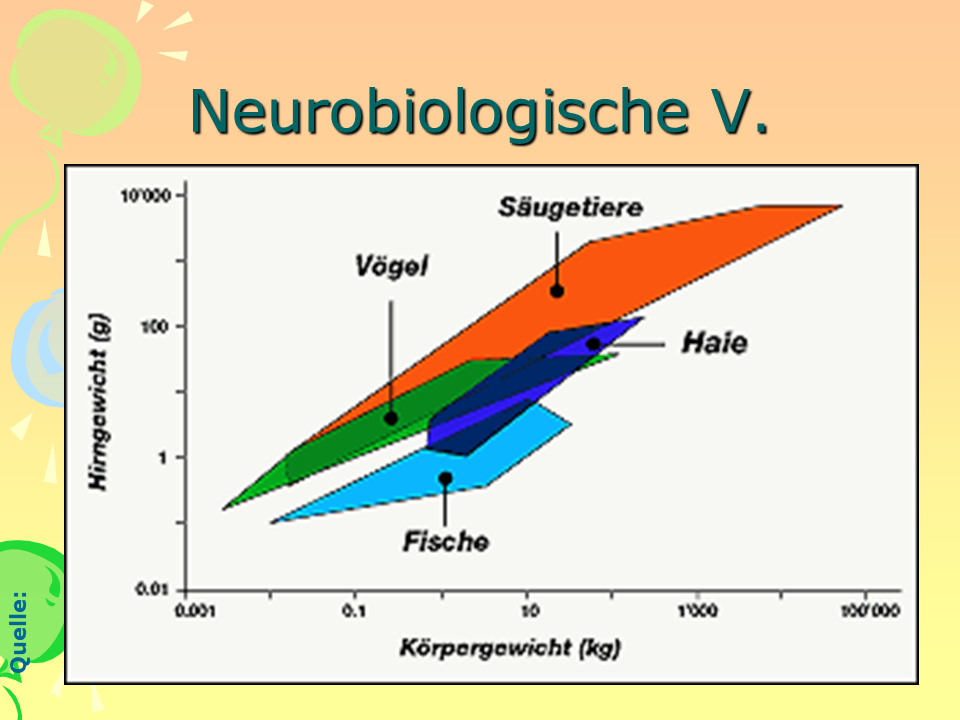
\includegraphics[width=1\textwidth,height=\textheight]{./pictures/neuro/Diapozitiv10.PNG}

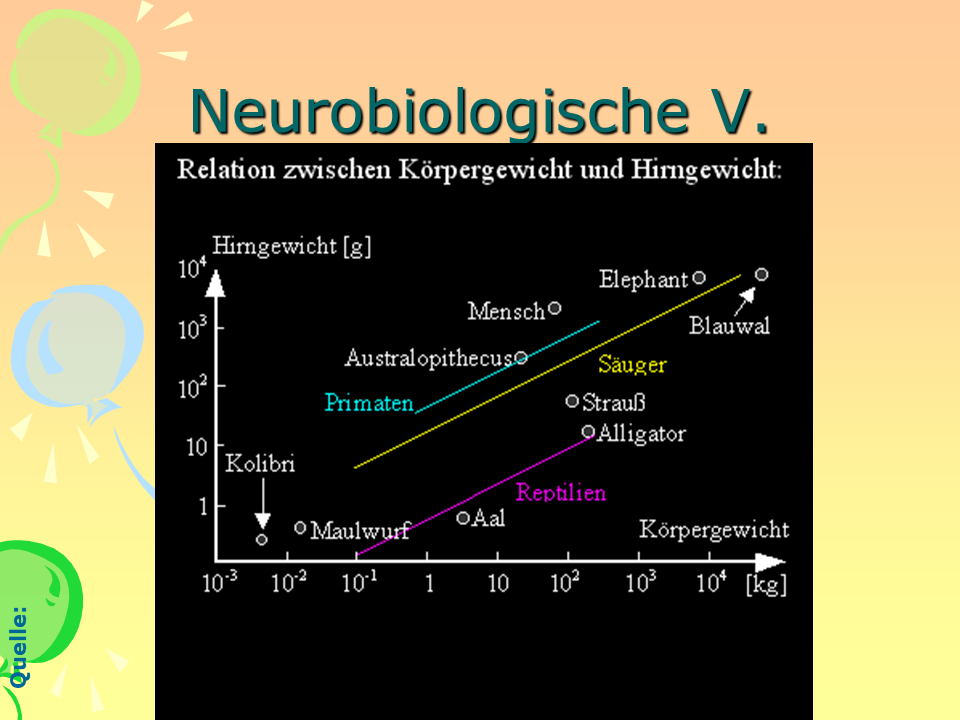
\includegraphics[width=1\textwidth,height=\textheight]{./pictures/neuro/Diapozitiv11.PNG}

\hypertarget{immer-online}{%
\section{Immer Online}\label{immer-online}}

Unser Gehirn ruht nie - ist immer ONLINE.

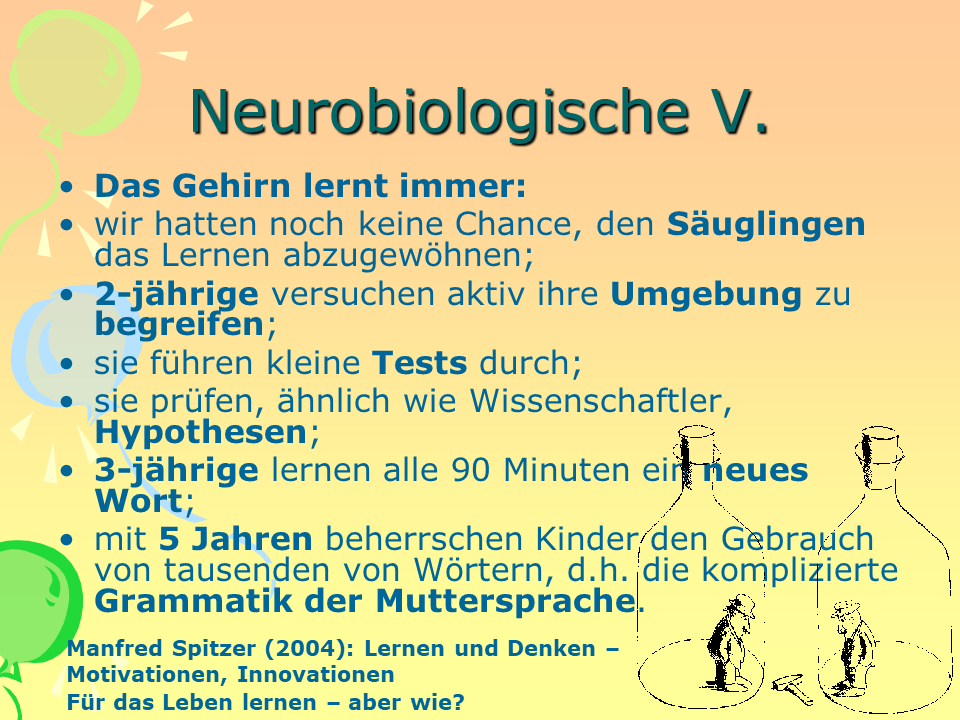
\includegraphics[width=1\textwidth,height=\textheight]{./pictures/neuro/Diapozitiv16.PNG}

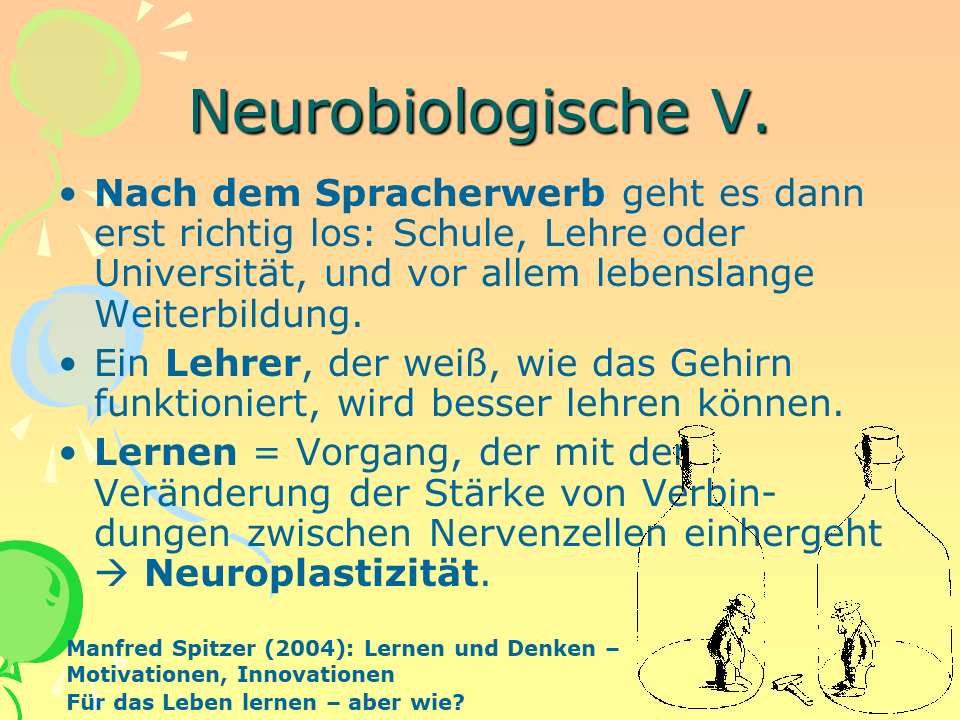
\includegraphics[width=1\textwidth,height=\textheight]{./pictures/neuro/Diapozitiv17.PNG}

\hypertarget{neuronale-netzwerke}{%
\section{Neuronale Netzwerke}\label{neuronale-netzwerke}}

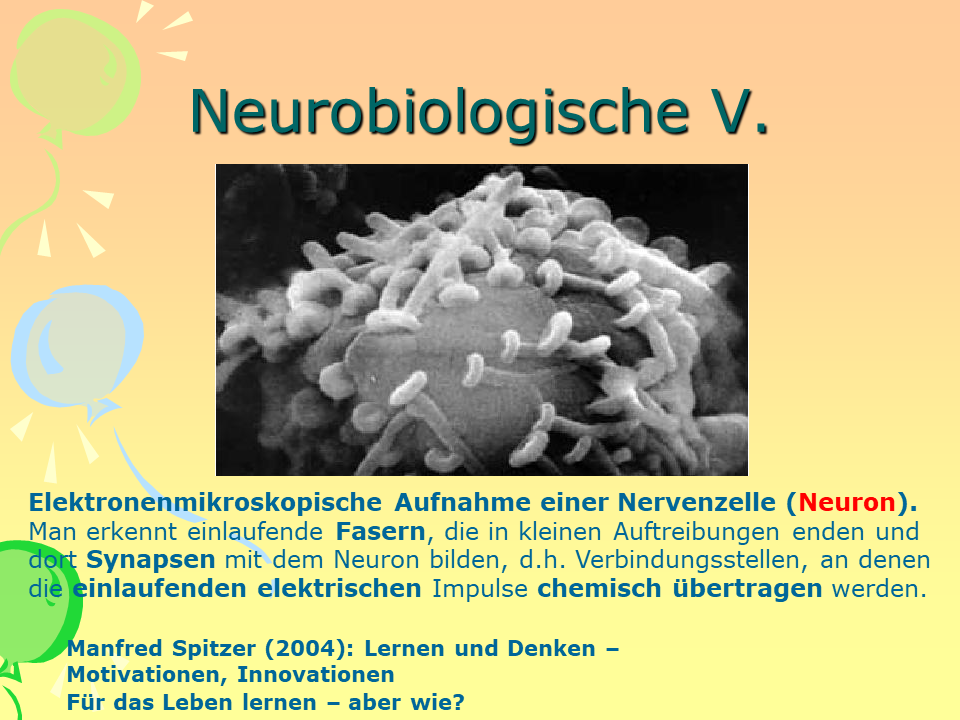
\includegraphics[width=1\textwidth,height=\textheight]{./pictures/neuro/Diapozitiv20.PNG}

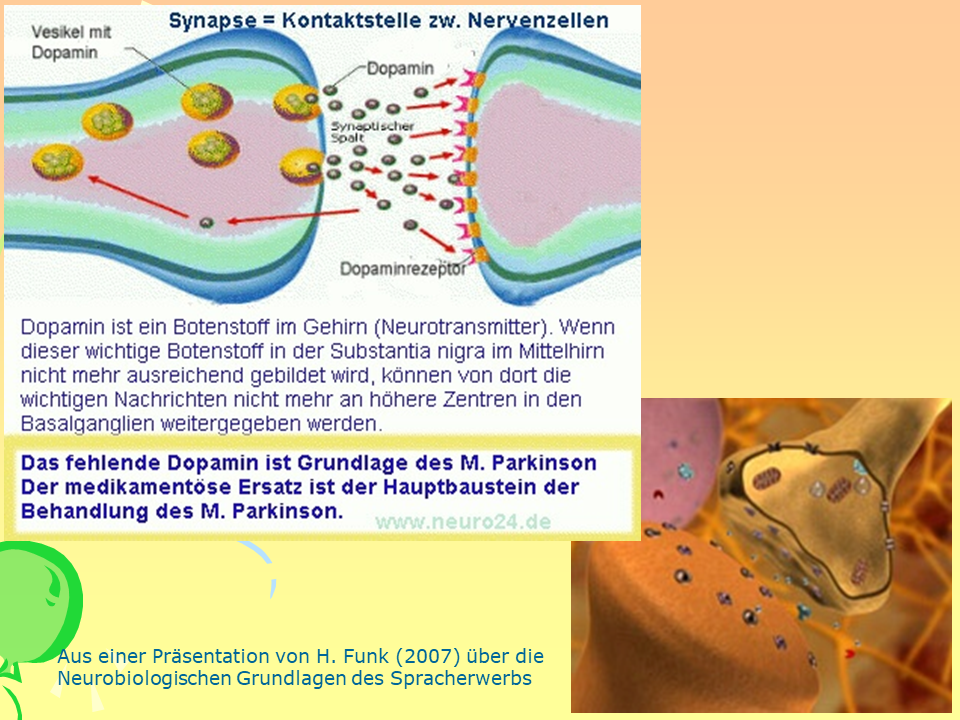
\includegraphics[width=1\textwidth,height=\textheight]{./pictures/neuro/Diapozitiv23.PNG}

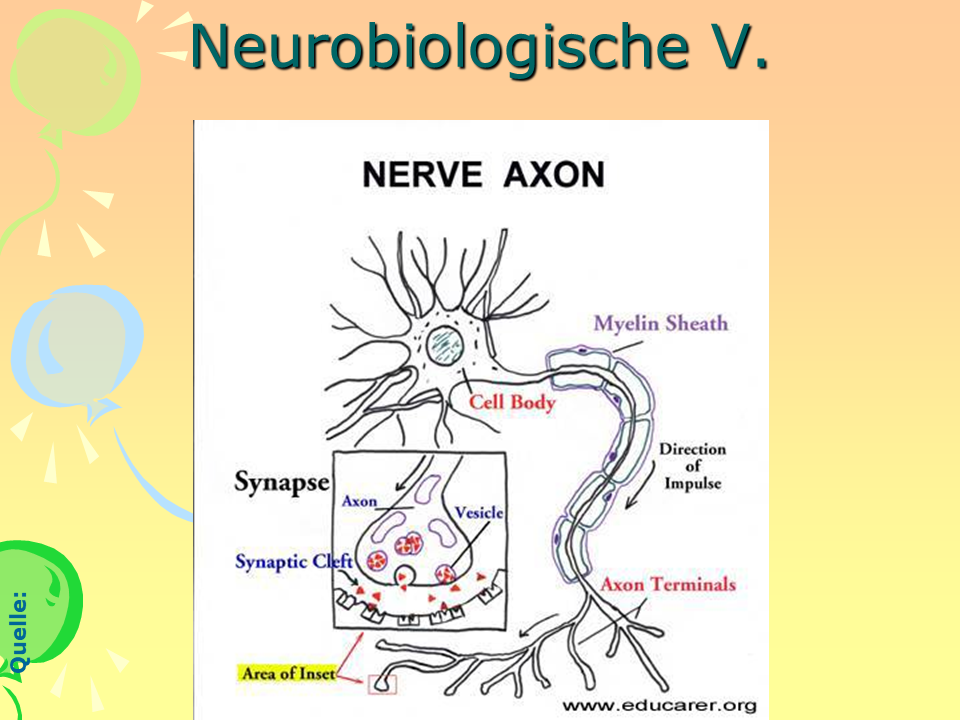
\includegraphics[width=1\textwidth,height=\textheight]{./pictures/neuro/Diapozitiv24.PNG}

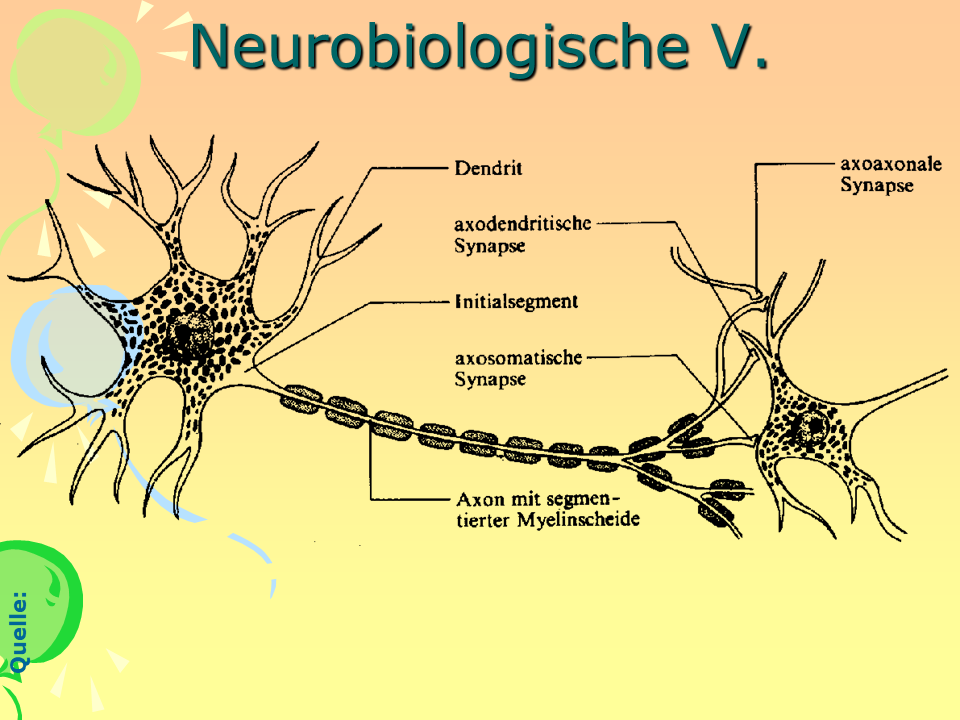
\includegraphics[width=1\textwidth,height=\textheight]{./pictures/neuro/Diapozitiv25.PNG}

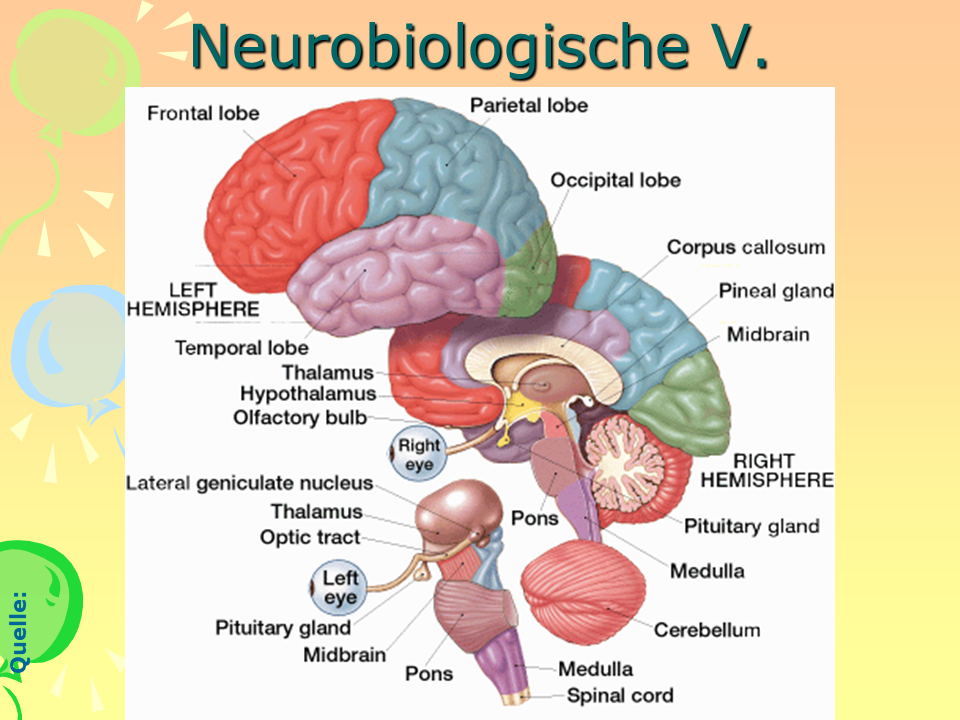
\includegraphics[width=1\textwidth,height=\textheight]{./pictures/neuro/Diapozitiv26.PNG}

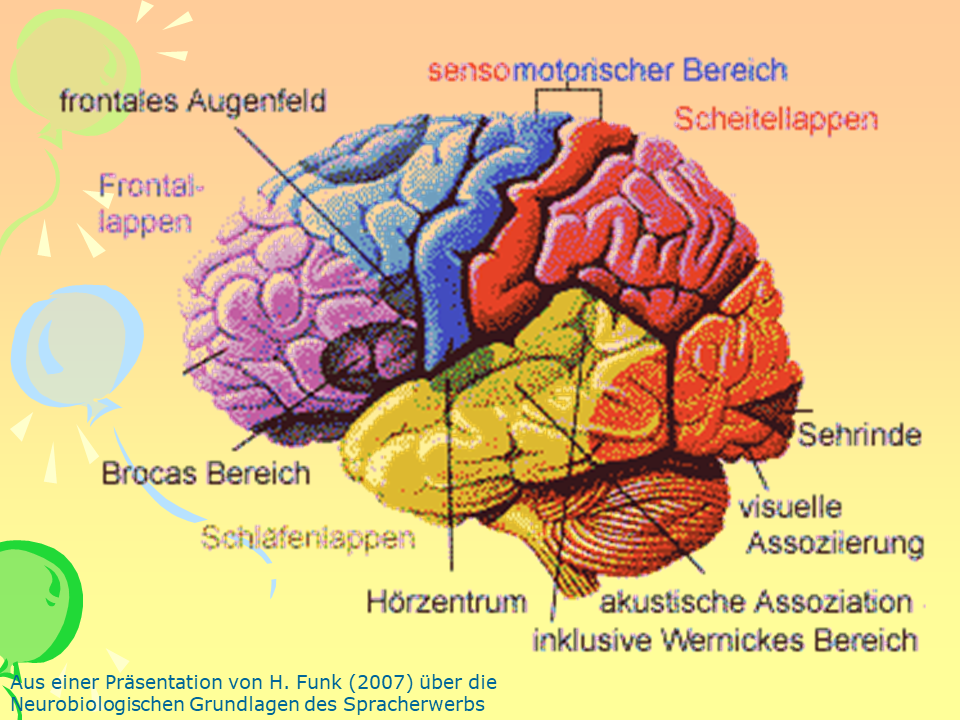
\includegraphics[width=1\textwidth,height=\textheight]{./pictures/neuro/Diapozitiv27.PNG}

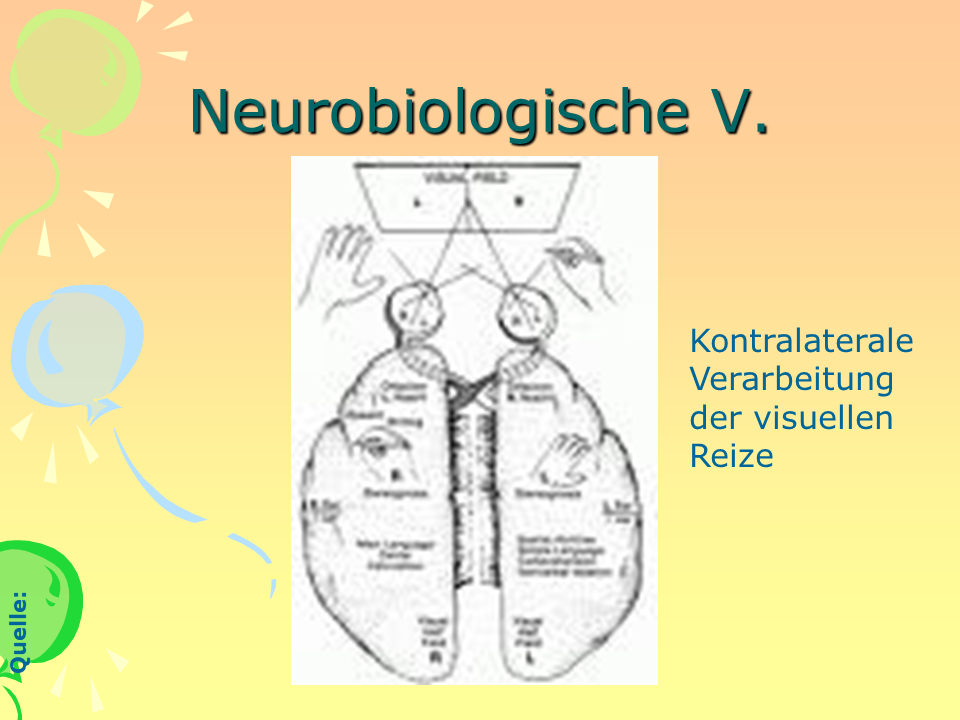
\includegraphics[width=1\textwidth,height=\textheight]{./pictures/neuro/Diapozitiv28.PNG}

\hypertarget{kortikale-landkarten}{%
\section{Kortikale Landkarten}\label{kortikale-landkarten}}

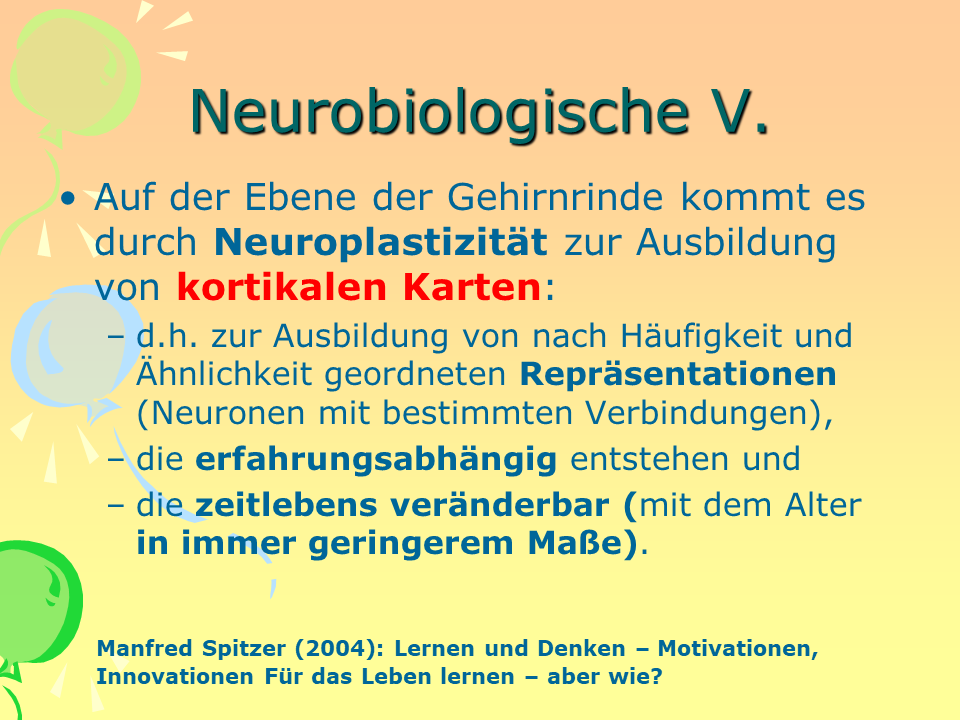
\includegraphics[width=1\textwidth,height=\textheight]{./pictures/neuro/Diapozitiv30.PNG}

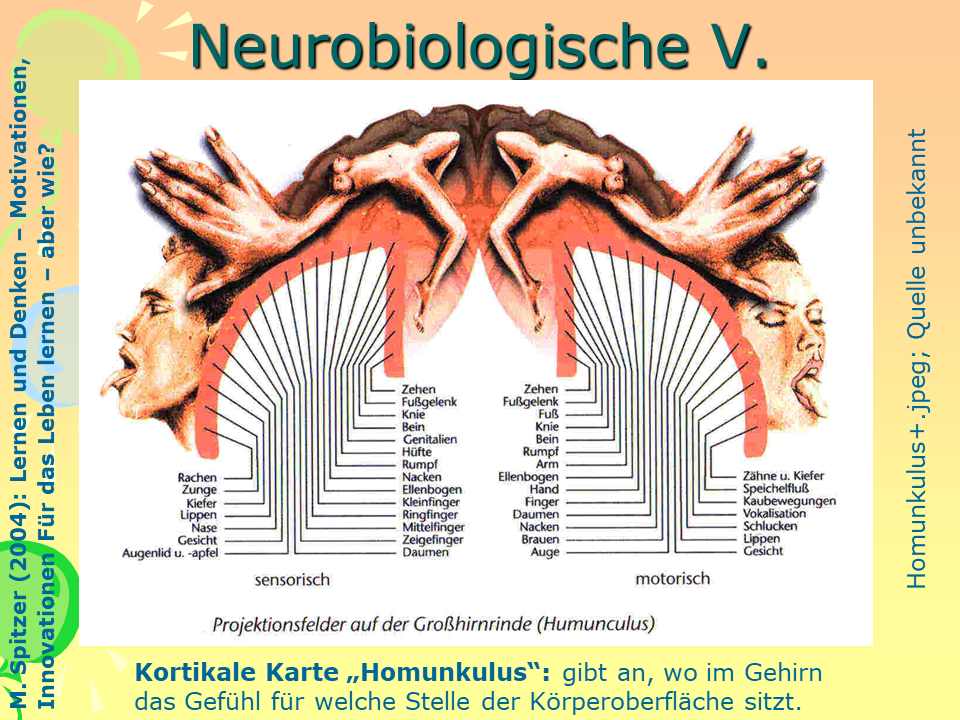
\includegraphics[width=1\textwidth,height=\textheight]{./pictures/neuro/Diapozitiv31.PNG}

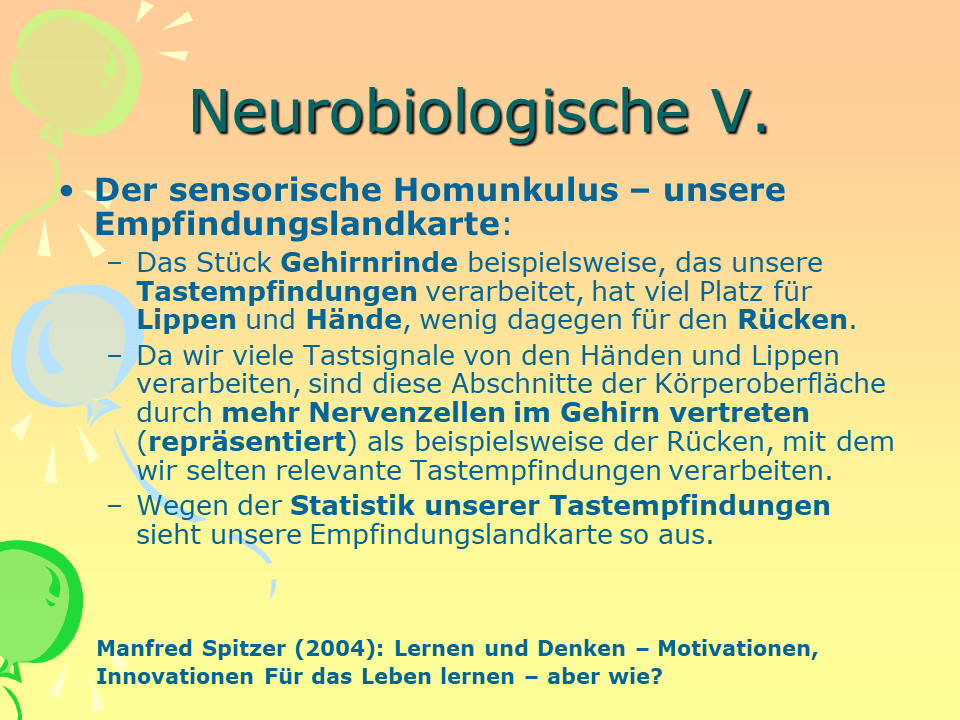
\includegraphics[width=1\textwidth,height=\textheight]{./pictures/neuro/Diapozitiv32.PNG}

\hypertarget{muster-und-intentionen}{%
\section{Muster und Intentionen}\label{muster-und-intentionen}}

Das Auge: Die rund 126 Mio. Zellen der Netzhaut liefern eine
unglaubliche Datenmenge ins Gehirn: pro Sekunde etwa 1,2 Megabyte. Das
entspricht einer Informationsmenge von 10.000 Seiten eines Buches.

Unser Gehirn versucht in den visuellen Reizen Muster zu erkennen, die an
bereits bekannte anknüpfen.

\textbf{Visuelle Muster}: Gestaltheorie - Figur vs.~Grund (Foregrounding
\& Backgrounding Processes)

\begin{figure}

{\centering 

\href{https://bildnerisches-gestalten.ch/index.php/wahrnehmung/}{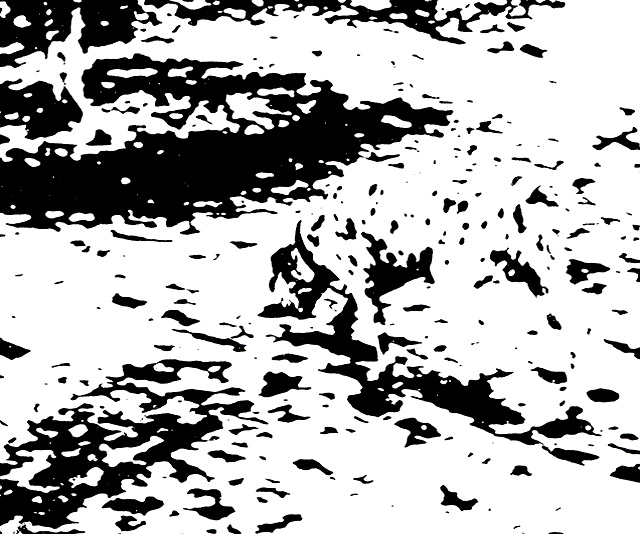
\includegraphics[width=1\textwidth,height=\textheight]{./pictures/dalmatiner.jpg}}

}

\end{figure}

Unser Gehirn versucht (holistische) Gestalten - Muster - zu erkennen,
wobei es sich auf Erfahrungswerte stützt und demnach zwischen
\textbf{Figur und Grund} unterscheidet (Vordergrund / Hintergrund). Die
Unterscheidung zwischen Figur und Grund fällt bei hohem Kontrast
leichter als bei geringem. Aus der anthropozentrischen Perspektive des
Menschen stellt stellt der Hund in dem Fleckenbild die Figur (den
Vordergrund) dar, die Umgebung dagegen den Hintergrund. Lebewesen werden
gewöhnlich als Figur interpretiert, da Lebewesen für Menschen
interessant bzw. besonders relevant sind und sich bewegen, während die
größere, statische Größe den Hintergrund bildet.

Akustische Reize (auch sprachliche) werden nach denselben Prinzipien
verarbeitet wie die visuellen Reize. In einem Satz, z.B. \emph{Der
Dalmatiner läuft durch den Wald,} wäre die Phrase \emph{der Dalmatiner}
dementsprechend die (wichtigere) Figur (der Vordergrund) und die Phrase
\emph{durch den Wald} der (weniger wichtige) Hintergrund der Aktion
(\emph{laufen}).

Zusammengestellt anhand von: - Stoll (2008)

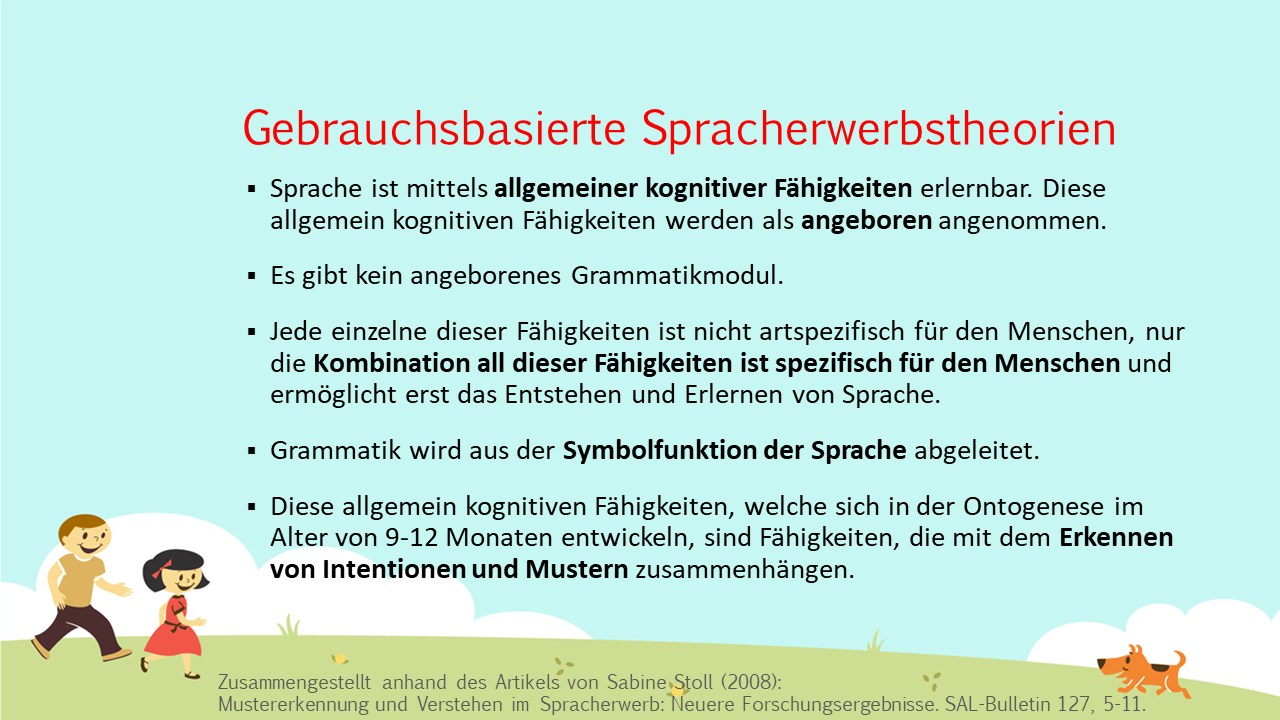
\includegraphics[width=1\textwidth,height=\textheight]{./pictures/muster_intentionen/Diapozitiv5.PNG}

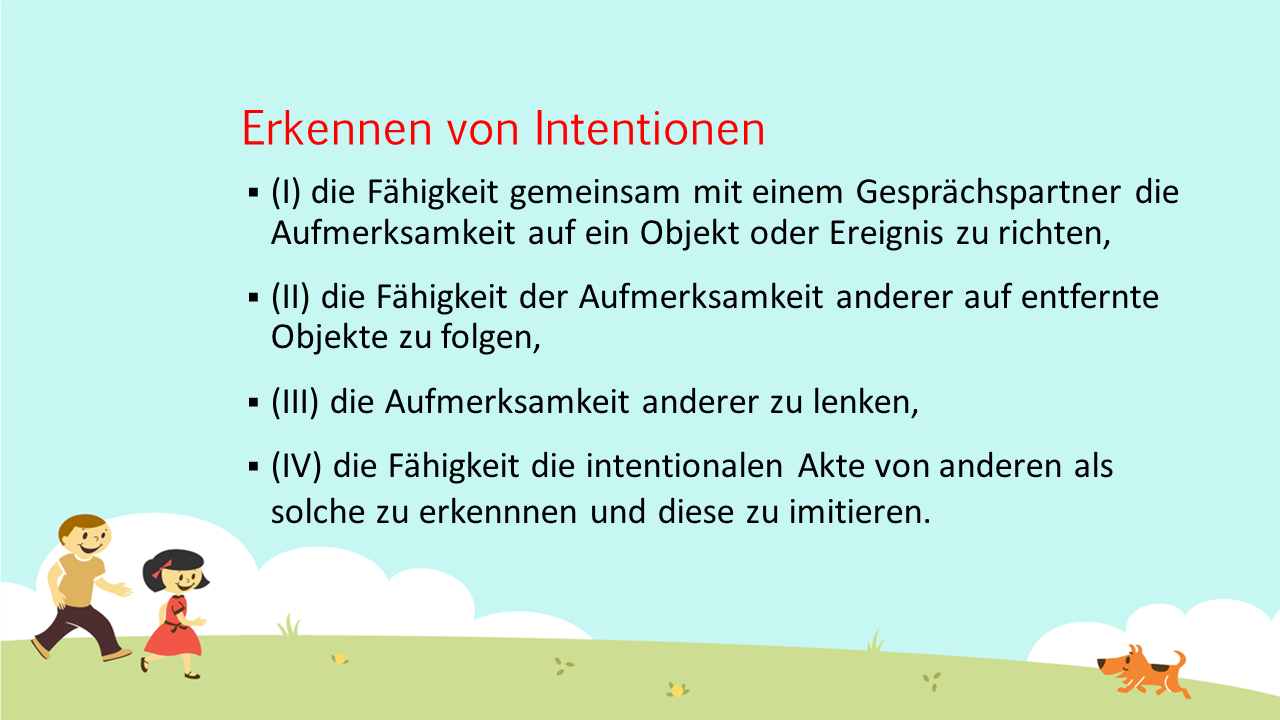
\includegraphics[width=1\textwidth,height=\textheight]{./pictures/muster_intentionen/Diapozitiv6.PNG}

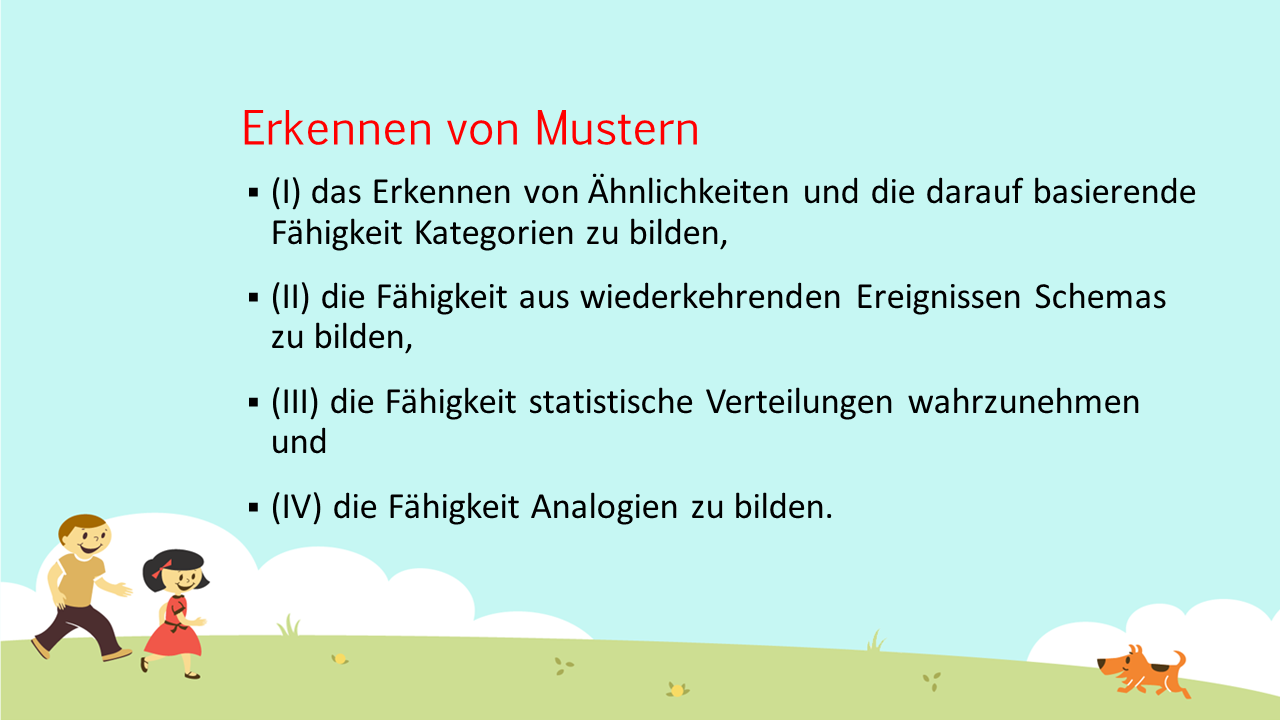
\includegraphics[width=1\textwidth,height=\textheight]{./pictures/muster_intentionen/Diapozitiv7.PNG}

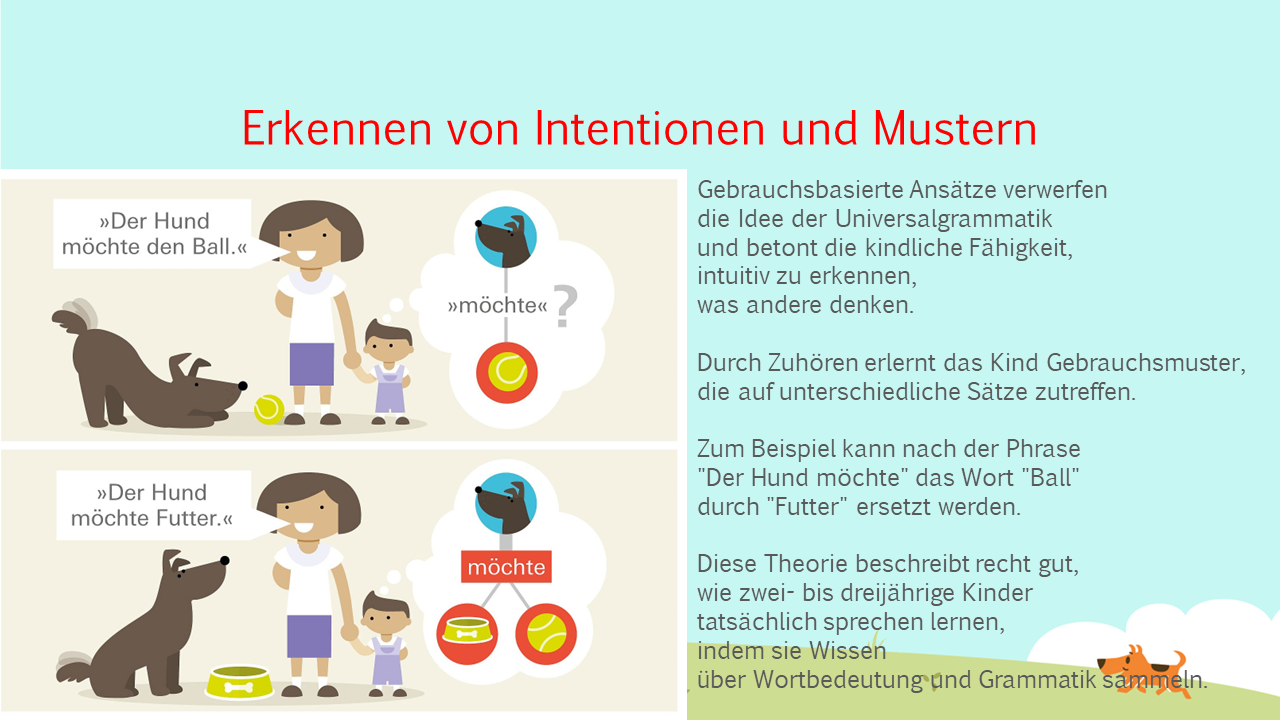
\includegraphics[width=1\textwidth,height=\textheight]{./pictures/muster_intentionen/Diapozitiv8.PNG}

\hypertarget{kategorienbildung}{%
\section{Kategorienbildung}\label{kategorienbildung}}

Beim Lernen bilden wir Kategorien, in die verschiedene Erscheinungen in
unserer Umwelt eingeordnet werden. Kategorien erleichtern Menschen den
Umgang mit ihrer Umwelt.

``\textbf{Kategorisierung} oder Kategorienbildung bezeichnet in der
Psychologie den Prozess, Objekte in Untergruppen oder Begriffsklassen
einzuteilen. (Stangl, 2023).''\\
\strut \\
Stangl, W. (2023, 13. März).
\href{https://lexikon.stangl.eu/7003/kategorisierung-kategorienbildung}{\emph{Kategorisierung
-- Kategorienbildung -- Online Lexikon für Psychologie \& Pädagogik}}.\\

\textbf{Kategorisierung} oder \textbf{kategoriales Denken} bezeichnet
die \href{https://de.wikipedia.org/wiki/Kognition}{kognitive} Fähigkeit,
unterschiedliche
\href{https://de.wikipedia.org/wiki/Entit\%C3\%A4t}{Entitäten}
(Gegenstände, Lebewesen, Vorgänge,
\href{https://de.wikipedia.org/wiki/Abstraktum}{Abstrakta})
\href{https://de.wikipedia.org/wiki/Intuition}{intuitiv} zu sortieren
und entsprechenden Sammelbegriffen (Kategorien) unterzuordnen. Diese
Kategorien basieren auf bestimmten Ähnlichkeiten oder auf dem Abgleich
mit dem theoretischen
Vor\href{https://de.wikipedia.org/wiki/Wissen}{wissen}. Die
Kategorienbildung ist ein fundamentaler Vorgang bei der Interpretation
und Bewertung von
\href{https://de.wikipedia.org/wiki/Wahrnehmung}{Wahrnehmungsinhalten},
dem Verständnis von Konzepten und
\href{https://de.wikipedia.org/wiki/Objekt_(Philosophie)}{Objekten}, bei
\href{https://de.wikipedia.org/wiki/Entscheidung}{Entscheidungsprozessen}
und bei allen Arten der Interaktion mit der
Umwelt.\textsuperscript{\href{https://de.wikipedia.org/wiki/Kategorisierung_(Kognitionswissenschaft)\#cite_note-Categorization-1}{{[}1{]}}}
Demzufolge sind Kategorien die „Grundbegriffe unseres
Denkens''.\textsuperscript{\href{https://de.wikipedia.org/wiki/Kategorisierung_(Kognitionswissenschaft)\#cite_note-Austeda-2}{{[}2{]}}}
{[}Kategorisierung{]}(https://de.wikipedia.org/wiki/Kategorisierung\_(Kognitionswissenschaft)

\begin{figure}

{\centering 

\href{https://www.keramikdeko.de/blog/alles-ueber-keramiktassen-und-keramikbecher-b74.html}{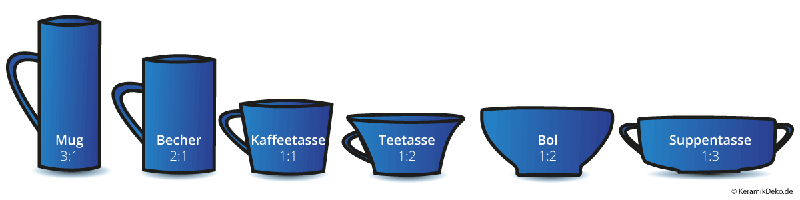
\includegraphics[width=1\textwidth,height=\textheight]{./pictures/Arten_von_Tassen_800.png}}

}

\end{figure}

\emph{Kategorielle Perzeption} von sprachlichen Stimuli: Die Suche nach
akustischen Hinweisen (engl. cues), die bei der Segmentierung größerer
Einheiten notwendig sind und die Aufdeckung von Kontrasten ermöglichen
(und damit Bedeutungsfindung). Gesucht wird nach distinktiven Merkmalen.
Akustische Signale sind (so wie visuelle Reize) höchstvariabel. Menschen
(bereits im Säuglingsalter) können sehr feine Unterschiede zwischen
akustischen Stimuli erkennen und sie für sprachliche Kategorisierung
nutzen.

\href{https://www.youtube.com/watch?v=8-fMLs-xCaA}{ListenLab} (Dauer:
15:00 Minuten):

\url{https://www.youtube.com/embed/8-fMLs-xCaA}

\href{https://www.youtube.com/watch?v=nNYhCP6NiUg}{ListenLab} (Dauer:
9:53 Minuten):

\url{https://www.youtube.com/embed/nNYhCP6NiUg}

\emph{Voice Onset Timing} im Englischen (vgl. mit Deutsch und
Slowenisch):\\
\href{https://www.youtube.com/watch?v=xR6FieNmWfg}{Isabel Cooke McKay}
(Dauer: 19:21 Minuten):

\url{https://www.youtube.com/embed/xR6FieNmWfg}

\href{https://www.youtube.com/watch?v=Kv6WBQVkHTo}{NPTEL IIT Guwahati}
(Dauer: 19:14 Minuten):

\url{https://www.youtube.com/embed/Kv6WBQVkHTo}

\hfill\break
Das Kleinkind ist schon früh in der Lage (vermutlich aufgrund seiner
genetischen Veranlagung) zwischen \textbf{sprachlichen und
nicht-sprachlichen Reizen} (Geräuschen) zu unterscheiden. Angeboren
scheint auch die \textbf{Denkfähigkeit}, also Begriffe zu entwickeln und
zu verarbeiten. Ebenfalls zur kognitiven Kapazität im weiteren Sinne
zählt die genetisch verankerte kognitive Anlage gehören (vermutlich
angeborene) \textbf{Mechanismen der Segmentierung} des sprachlichen
Schallstroms anhand bestimmter akustischer Eigenschaften, die Fähigkeit
zur \textbf{Kategorisierung} sprachlicher, etwa formal und/oder
funktional identischer Eigenschaften wahrscheinlich unter Anwendung
distributioneller Analyseverfahren, die Voraussetzung für die
Entwicklung von Strategien zur Analyse struktureller Eigenschaften von
Äußerungen aus den Morphemen und ihrer linearen Anordnung etc. Man wird
diesen Teil der kognitiven Ausstattung in der Literatur auch unter der
Bezeichnung \textbf{Angeborenes sprachliches Wissen} antreffen. Weniger
direkt als alle bisher erwähnten kognitiven Voraussetzungen, aber
vielleicht für die Sprachfähigkeit am ehesten eine Schlüsselfähigkeit
stellt das leistungsfähige \textbf{Gedächtnis} des Menschen dar. Eine
Schlüsselrolle kommt ihm insofern zu, als es die Begriffsbildung und die
komplizierten Analysevorgänge überhaupt erst möglich macht.\\

\hypertarget{sprachliches-wissen}{%
\section{Sprachliches Wissen}\label{sprachliches-wissen}}

``Viele Arten haben die Fähigkeit zweckmäßig und eindeutig zu
kommunizieren und jede verwendet dazu ein je artspezifisches System. Die
Kommunikationsverfahren sind bestimmt von biologischen, sozialen und
kognitiven Voraussetzungen der jeweiligen Art und ihrer Lebenswelt. Und
die artspezifischen Sprachen sind es auch -- aber anders; Hauser (1996).
Die Kommunikationsverfahren sind angepasst einerseits an die peripheren
Organe der Produktion und Rezeption, andererseits an die psychischen
Repräsentationen der jeweiligen Organismen.'' - Dietrich (2002)

``Das \textbf{sprachliche Wissen} stellt dem Menschen die Mittel für die
sprachliche Kommunikation über nicht-sprachliche psychische Dinge
bereit, und die Organisation dieses Wissensbestandes prägt alle
Modalitäten der sprachlichen Verständigung.'' - Dietrich (2002)

Zum sprachlichen Wissen gehören Kenntnisse der Inhalts- und der
Ausdrucksseite:

\begin{itemize}
\item
  semantische Kenntnisse (Konzepte),
\item
  das Erkennen und die Unterscheidung von Äußerungsabsichten,
\item
  die Kenntnis der Worteigenschaften (syntaktische, morphologische,
  phonologische, graphematische Eigenschaften von Wörtern und ihren
  Verbindungen zu größeren Einheiten),
\item
  Textmusterwissen.
\end{itemize}

\hypertarget{das-mentale-lexikon}{%
\subsection{Das mentale Lexikon}\label{das-mentale-lexikon}}

Mit dem \textbf{mentalen Lexikon} meint man das sprachliche Wissen im
Langzeitgedächtnis.

Sind sprachliche Einheiten (Informationsbündel - chunks) wirklich als
\textbf{Einheiten} im \textbf{Langzeitgedächtnis} gespeichert? Wenn das
der Fall ist, so müssten sie auch als Einheit verarbeitet werden, also
anders als die im Informationsbündel enthaltenen Bestandteile. -
Dietrich (2002)

Wird eine so grundlegende sprachliche Einheit wie das \textbf{Wort als
Einheit} in unserem Langzeitgedächtnis gespeichert?

\textbf{Worthaftigkeitseffekt} (Wortüberlegenheitseffekt - Word
Superiority Effect):

Die Sprachrezeption erlaubt eher einen kontrollierten Zugang zu den
Verarbeitungsprozessen im Gehirn als die Sprachproduktion. Insbesondere
das Lesen ist relativ leicht zu kontrollieren und zu beobachten. Das
Lesen beginnt mit der visuellen Wahrnehmung der Buchstaben. Diese müssen
kurzfristig in einem begrenzten Speicher aufgenommen werden. Dies nimmt
Zeit in Anspruch. Eine einfache Annahme ist, das Lesen eines Buchstaben
schneller geht als das Lesen von zwei oder mehreren. Aber man hat
beobachtet, dass in manchen Fällen die Verarbeitung eines Buchstaben
länger dauern kann als die von zwei oder mehreren. Dies hat man vor
allem bei Buchstabenfolgen bemerkt, die kurze Wörter darstellen. Handelt
es sich nun um einen allgemeinen Worthaftigkeitseffekt oder nur um eine
Eigenschaft spezieller Wörter?

Bei der Überprüfung zeigt sich zunächst, dass die Lesegeschwindigkeit
für Buchstabenfolgen, die Wörter bilden, kürzer ist als für Nichtwörter.
Dies kann mit der \textbf{Worthaftigkeit} erklärt werden \textbf{oder}
auch mit der \textbf{Wahrscheinlichkeit} der Abfolge von Buchstaben in
einer Sprache. Im letzteren Fall würde es sich um einen
\textbf{Häufigkeitseffekt} auf Buchstabenebene handeln und nicht um
einen Worthaftigkeitseffekt.

\textbf{Experiment zum Nachweis des Wortüberlegenheitseffekts} (Reicher
1969):

In schneller Folge und sehr kurz werden eine Buchstabenfolge, MAUS (=
Wortbedingung) oder AMUS (Non-Wort-Bedingung) und sodann eine
entsprechende maskierte Buchstabenfolge, z.B. MAU bzw. AMU gezeigt.

Welcher Buchstabe an der maskierten Position stand, kann nach sehr
kurzer Lesezeit (\textless= 100 ms) nicht aus der Erinnerung abgerufen
werden.

Dann folgt die Aufgabe: Es wird der Buchstabe S oder L gezeigt und die
Entscheidung verlangt, ob es der letzte Buchstabe der zuerst gesehenen
Folge, also MAUS bzw. AMUS war.

\textbf{Ergebnis}: Die Entscheidung ist unter Wort-Bedingung signifikant
häufiger korrekt als unter Nicht-Wort-Bedingung, und zwar obwohl beide
Buchstaben (S und L) auf den Buchstaben ``a'' gleich häufig folgen und
zu einem Wort ergänzen. Bei Wahrnehmung eines Wortes wird das
lexikalische Wissen abgerufen. Dadurch wird das Lesen von Wörtern
beschleunigt.\\

Versuchspersonen lasen Buchstabenfolgen (\textbf{Wörter}, Non-Wörter und
sog. Pseudo-Wörter), die jeweils sehr kurz visuell präsentiert wurden
(Ripamonti et al.~(2014)). Sie lasen die Buchstabenfolgen einmal mit dem
linken Auge (kontralaterale Verarbeitung über die rechte Gehirnhälfte),
einmal mit dem rechten (kontralaterale linkshemisphärische
Verarbeitung).

Ein \textbf{Pseudo-Wort} ist eine Buchstabenfolge, die nach den
phonotaktischen Regeln in der jeweiligen Sprache ein Wort darstellen
könnte, aber keine Bedeutung hat und nicht im mentalen Lexikon enthalten
ist. Ein \textbf{Nicht-Wort} ist eines, das ebenfalls ohne Bedeutung und
nicht im mentalen Lexikon vorhanden ist und dessen Buchstabenfolge nicht
den phonotaktischen Regeln folgt.

Im Deutschen ist z. B.

\begin{itemize}
\item
  h-a-u-s ein Wort,
\item
  h-a-u-m ein Pseudowort und
\item
  h-s-u-a ein Nicht-Wort.
\end{itemize}

\textbf{Ergebnis}: An Nicht-Wörter erinnerten sich die Versuchspersonen
schlechter als an Wörter und Pseudowörter. Zwischen Wörtern und
Pseudowörtern (des Italienischen) fand man keinen wesentlichen
Unterschied.

\textbf{Schlussfolgerung}: Beim Lesen sind \textbf{prälexikalische}
Prozesse beteiligt (d.h. ein Zugriff auf das mentale Lexikon ist nicht
notwendig). Dies wird dadurch bestätigt, dass es zwischen linkem und
rechtem Auge keinen wesentlichen Unterschied gab (also Prozesse über die
linke als auch über die rechte Gehirnhälfte ablaufen können).

\textbf{Stroop-Effekt}: Dieser Effekt bestätigt ebenfalls den
Worthaftigkeitseffekt, denn Buchstabenfolgen, die ein Wort ergeben,
werden automatisch als Wort verarbeitet. Die Verarbeitung ist so stark
automatisiert, dass man die Verarbeitung kaum unterdrücken kann.

Mit der Bezeichnung \emph{Stroop-Effekt} bezieht man sich auf mehrere
Reaktionsmuster bei Aufgaben:

\begin{enumerate}
\def\labelenumi{\arabic{enumi}.}
\item
  die Farbe einer Fläche zu nennen,
\item
  eine Farbbezeichnung zu lesen, die mit der Schriftfarbe kongruiert
  (übereinstimmt),
\item
  eine Farbbezeichnung zu lesen, die mit der Schriftfarbe nicht
  kongruiert (kontrastiert),
\item
  die Schriftfarbe einer nicht-kongruenten Farbbezeichnung zu nennen.
\end{enumerate}

Der Vergleich der Bedingungen 2 und 3 zeigt den (geringen) Effekt der
Farbe auf das Lesen eines Wortes, der Vergleich von 1 und 4 den
Interferenzeffekt, der durch die Bedeutung des Farbwortes ausgelöst wird
und die Benennung der Farbe beeinträchtigt.

Verglichen werden die Lesezeiten unter den vier verschiedenen
Bedingungen.

Zwischen Wortbedeutung und Farbvorstellung gibt es demnach einen
Interferenzeffekt. Die sprachliche Einheit des Wortes zwingt das Denken,
sich mit seiner Verarbeitung zu beschäftigen und beeinträchtigt die
Verarbeitung der Farbwahrnehmung. - Dietrich (2002)

Es gibt zahlreiche Versionen des Stroop-Experiments, der
Interferenzeffekte aufdeckt. --\textgreater{} Pinkers Vortrag bei Google
(YouTube).

Dietrich (2002): Bearbeiten !!!!

\textbf{Lauterkennung im Wortkontext} und Phonemrestauration: Auch die
Verarbeitung von Lauten wird davon beeinflusst, ob der Laut als
Bestandteil eines Wortes gehört wird oder nicht. Unter anderem wird die
Fähigkeit davon beeinflusst, Urteile über auditiv Wahrgenommenes zu
fällen. Wird in einem gehörten Wort ein Laut einmal mit Geräusch
überlagert, ein andermal durch Geräusch vollständig ersetzt, so wird
letzteres schlechter erkannt. Dieser Effekt tritt nicht auf beim Hören
gleichartig unterschiedener Nicht-Wort-Paare (vgl. Samuel 1986).

Der Effekt der sog. \textbf{Phonemrestauration} (phonemic restoration
effect) liefert Evidenz für dieselbe Annahme (vgl. Warren 1970;
Sivonen/Maess/ Lattner/Friederici 2006; Kashino 2006). Wird ein Laut
eines Wortes vollständig von einem nicht-sprachlichen Laut überlagert,
fällt dies Hörern bei der Wahrnehmung nicht notwendigerweise auf.
Versuchspersonen geben sogar an, den Laut deutlich gehört zu haben. Je
nach Kontext, ersetzen Hörer einen fehlenden Laut sogar in verschiedener
Weise (s. Kapitel 5 für eine detaillierte Erläuterung)\\

\textbf{Wortfrequenz}: Auch der Frequenzeffekt stützt die Annahme von
der kognitiven Realität des Wortes. Ein Wort, das in der täglichen
Kommunikation zwischen Mitgliedern der Sprachgemeinschaft häufig
verwendet wird, wird vom Einzelnen schneller verarbeitet. Die Frequenz
ist also eine Eigenschaft des Wortes und sie lässt sich nicht aus der
Frequenz seiner Laute ableiten. Der Frequenzeffekt zählt mit zu den
stabilsten Phänomenen lexikalischer Verarbeitung (vgl. Jescheniak/Levelt
1994; Jescheniak 2002; Graf/ Nagler/Jacobs 2005; jedoch auch
Jescheniak/Meyer/Levelt 2003b).\\

\hfill\break

\hypertarget{sprachareale}{%
\section{Sprachareale}\label{sprachareale}}

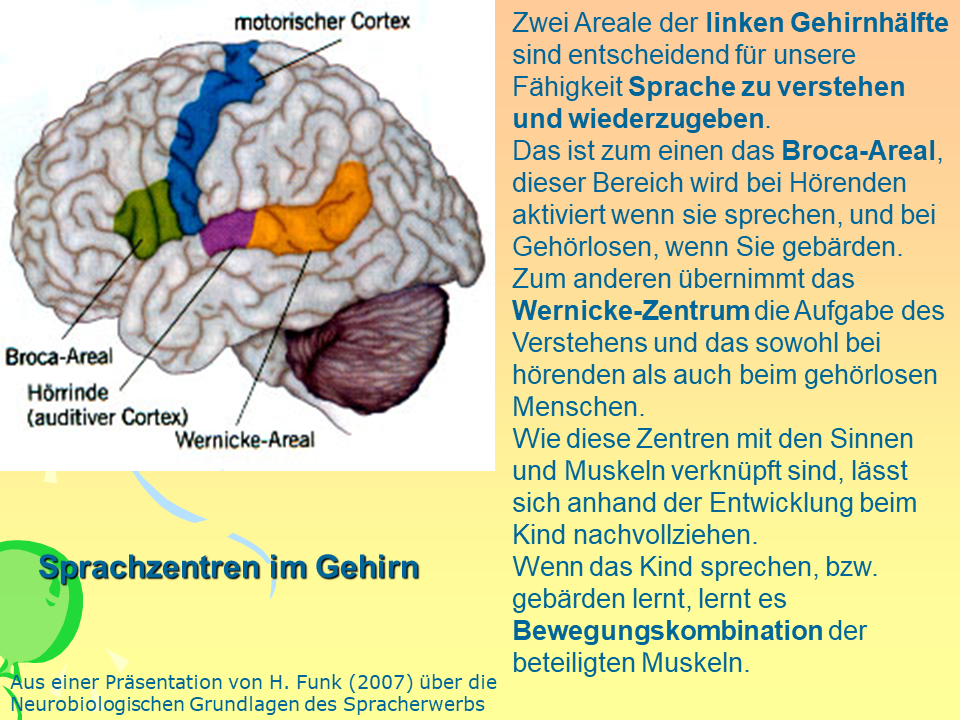
\includegraphics[width=1\textwidth,height=\textheight]{./pictures/neuro/Diapozitiv35.PNG}

\hypertarget{geduxe4chtnissysteme}{%
\section{Gedächtnissysteme}\label{geduxe4chtnissysteme}}

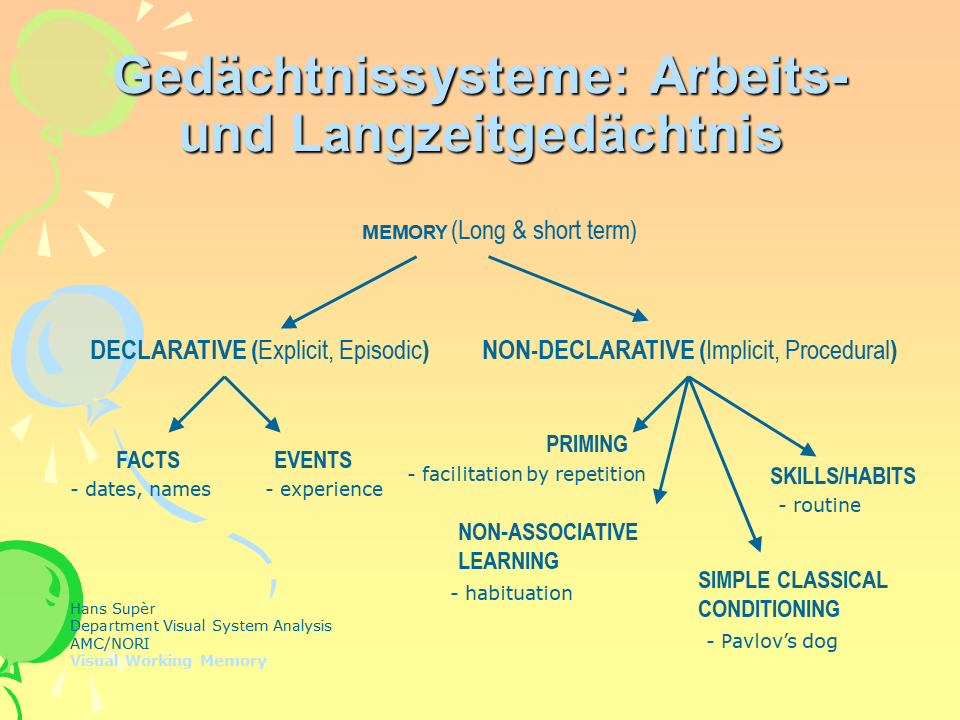
\includegraphics[width=1\textwidth,height=\textheight]{./pictures/neuro/Diapozitiv37.PNG}

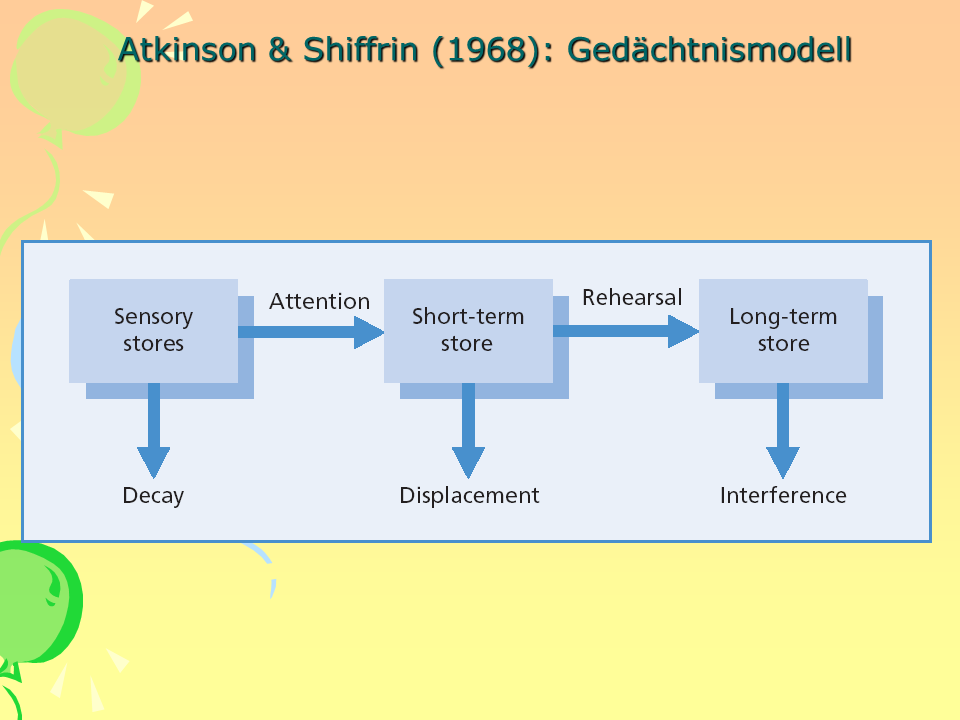
\includegraphics[width=1\textwidth,height=\textheight]{./pictures/neuro/Diapozitiv38.PNG}

\hypertarget{sensorisches-geduxe4chtnis}{%
\subsection{Sensorisches Gedächtnis}\label{sensorisches-geduxe4chtnis}}

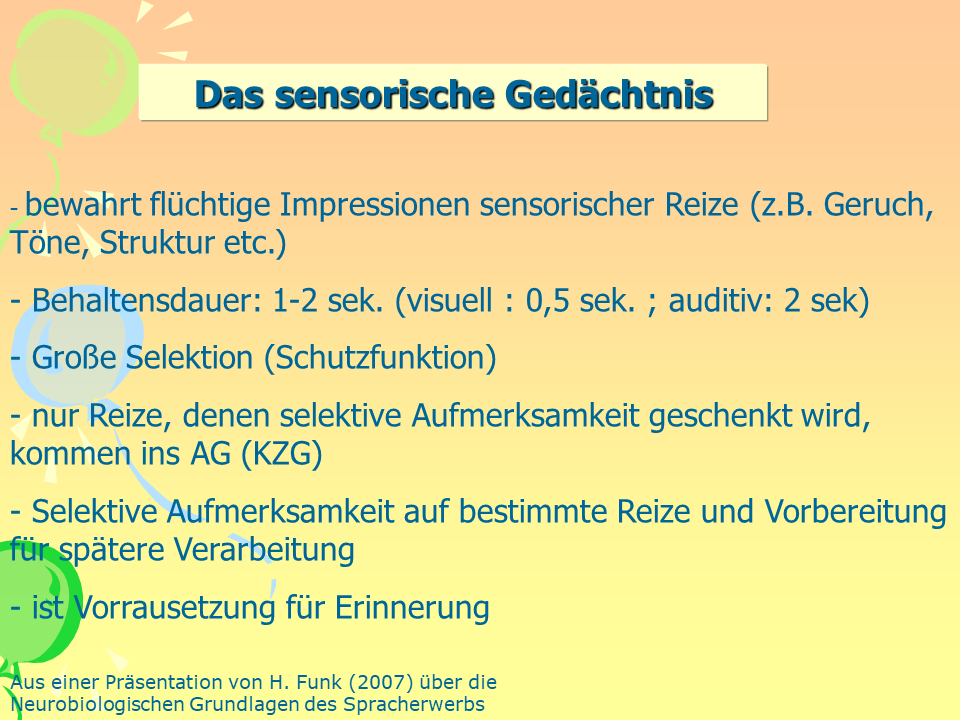
\includegraphics[width=1\textwidth,height=\textheight]{./pictures/neuro/Diapozitiv39.PNG}

\hypertarget{arbeitsgeduxe4chtnis}{%
\subsection{Arbeitsgedächtnis}\label{arbeitsgeduxe4chtnis}}

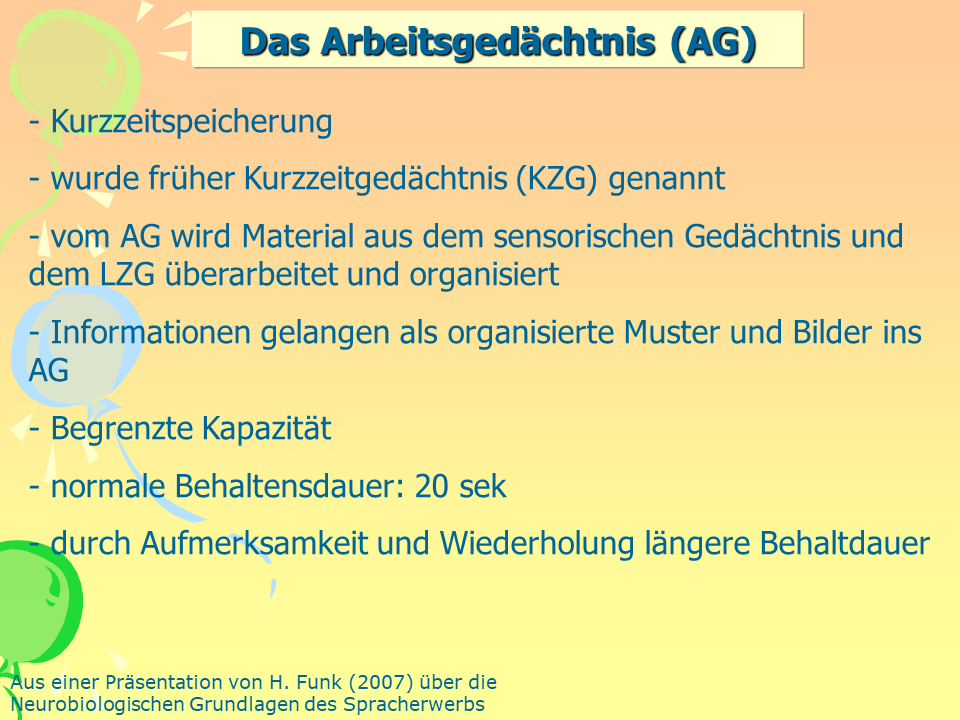
\includegraphics[width=1\textwidth,height=\textheight]{./pictures/neuro/Diapozitiv40.PNG}

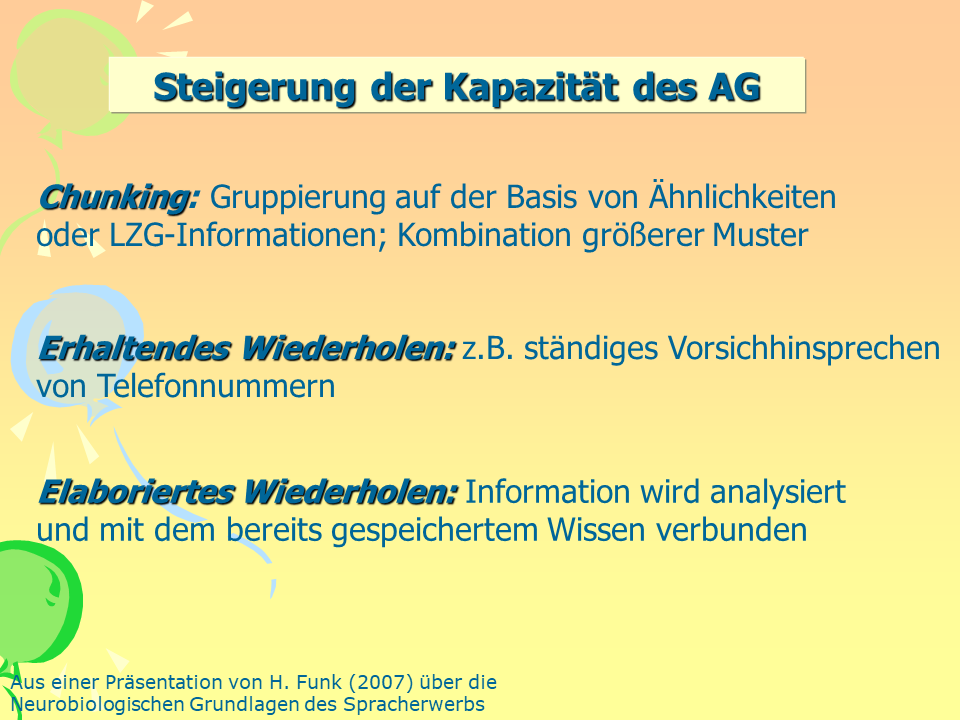
\includegraphics[width=1\textwidth,height=\textheight]{./pictures/neuro/Diapozitiv41.PNG}

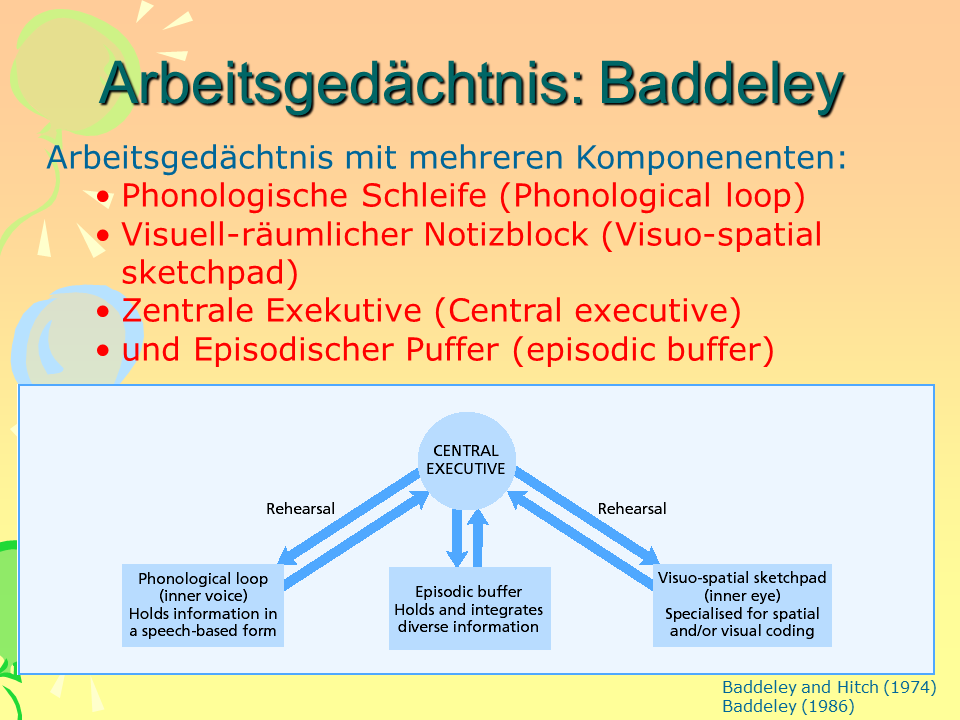
\includegraphics[width=1\textwidth,height=\textheight]{./pictures/neuro/Diapozitiv42.PNG}

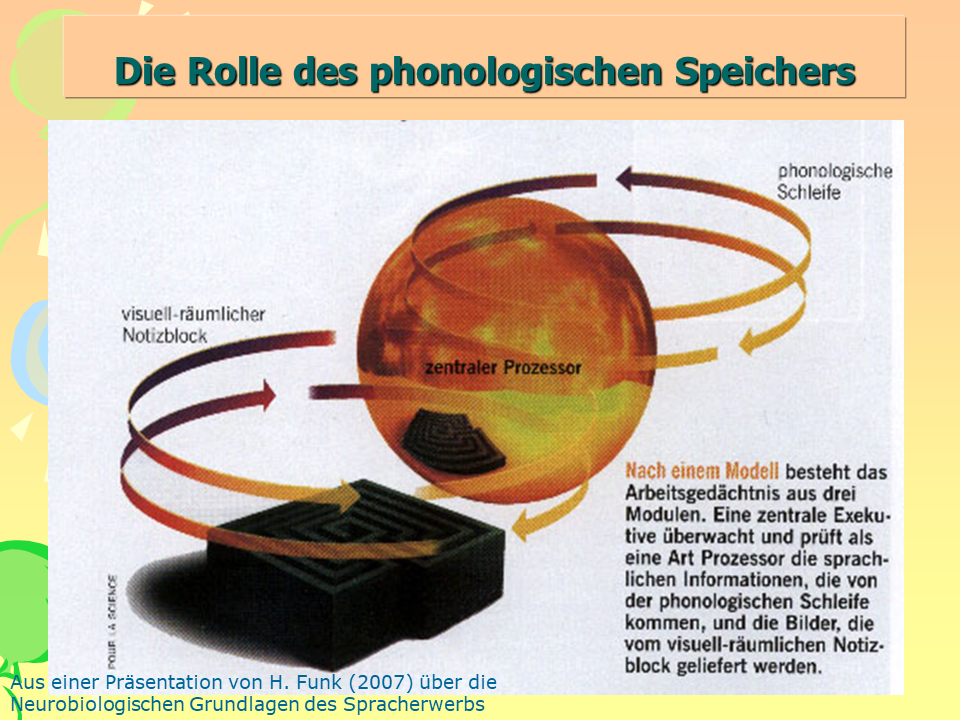
\includegraphics[width=1\textwidth,height=\textheight]{./pictures/neuro/Diapozitiv43.PNG}

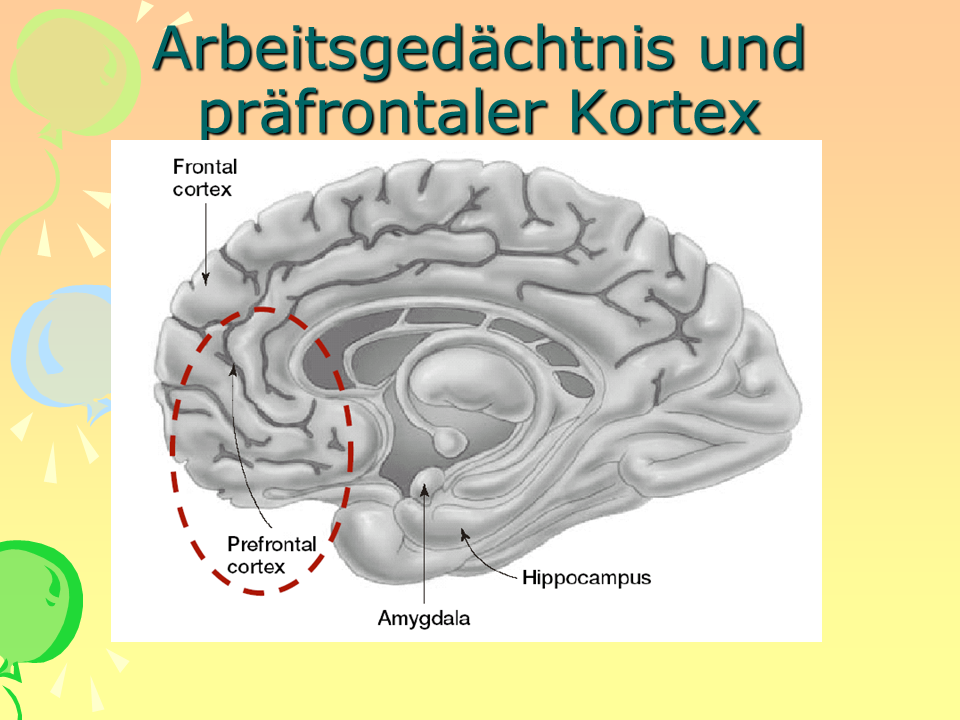
\includegraphics[width=1\textwidth,height=\textheight]{./pictures/neuro/Diapozitiv44.PNG}

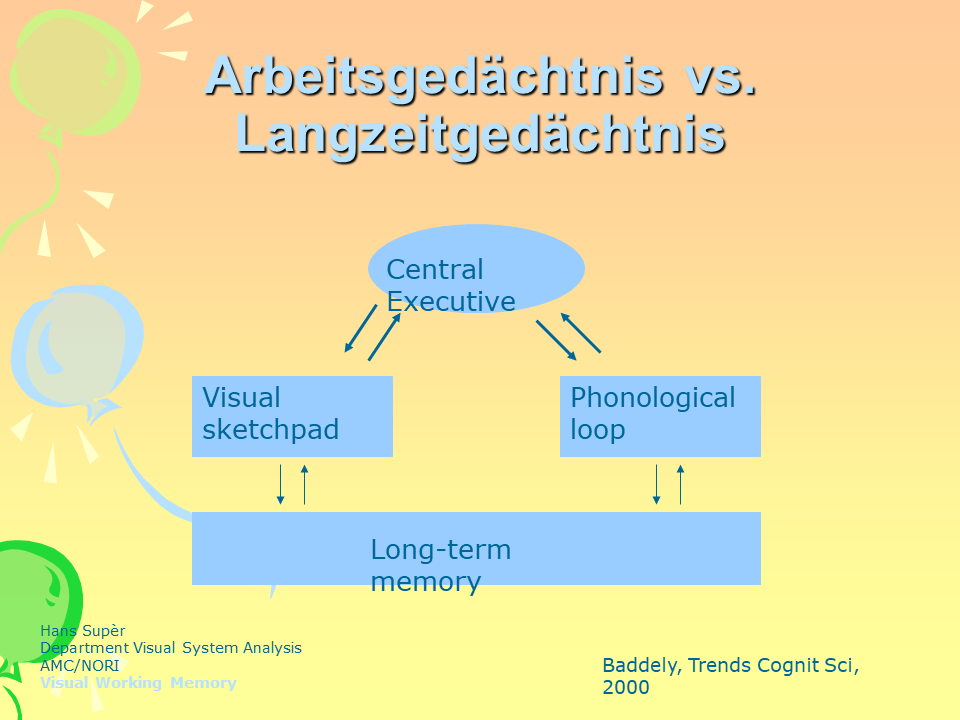
\includegraphics[width=1\textwidth,height=\textheight]{./pictures/neuro/Diapozitiv45.PNG}

\hypertarget{langzeitgeduxe4chtnis}{%
\subsection{Langzeitgedächtnis}\label{langzeitgeduxe4chtnis}}

\hypertarget{regeln}{%
\subsubsection{Regeln}\label{regeln}}

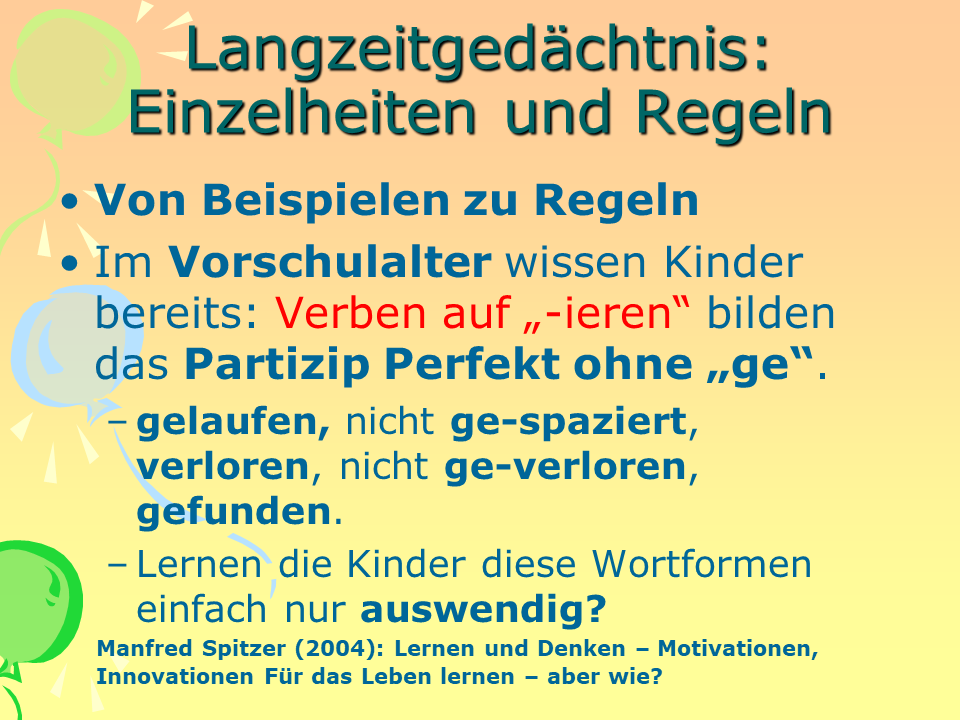
\includegraphics[width=1\textwidth,height=\textheight]{./pictures/neuro/Diapozitiv46.PNG}

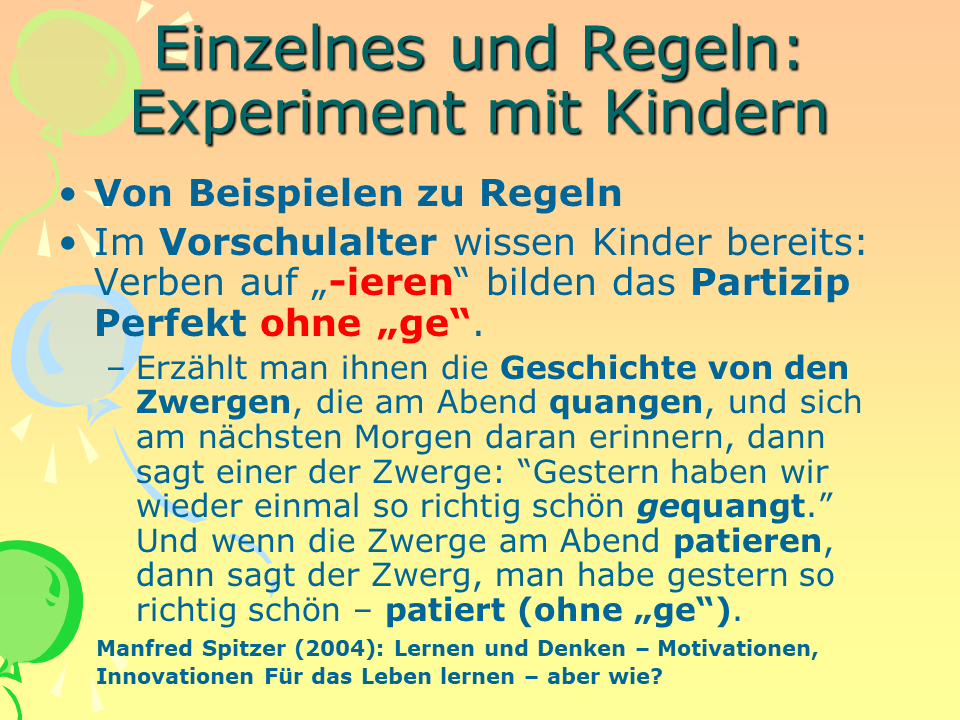
\includegraphics[width=1\textwidth,height=\textheight]{./pictures/neuro/Diapozitiv47.PNG}

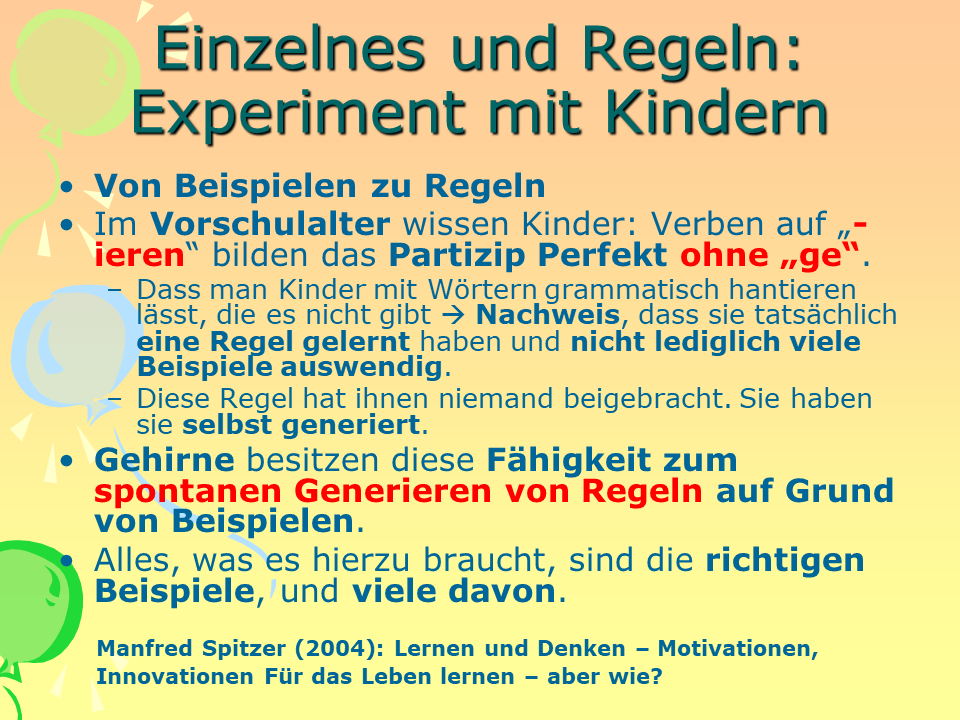
\includegraphics[width=1\textwidth,height=\textheight]{./pictures/neuro/Diapozitiv48.PNG}

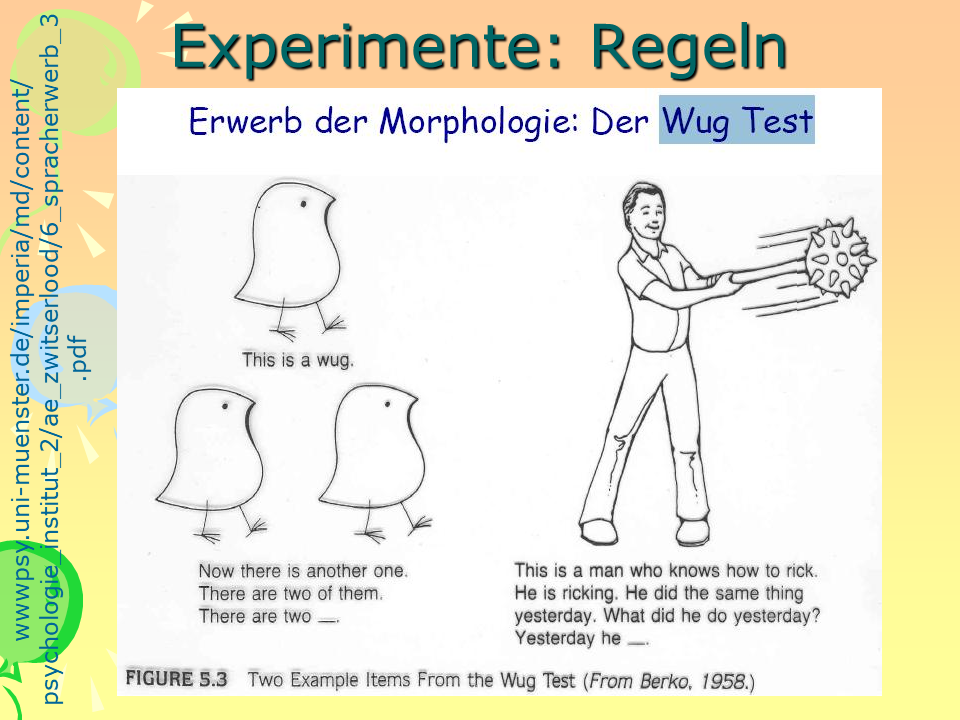
\includegraphics[width=1\textwidth,height=\textheight]{./pictures/neuro/Diapozitiv49.PNG}

\includegraphics[width=1\textwidth,height=\textheight]{./pictures/neuro/Diapozitiv50.PNG}

\hypertarget{einzelheiten}{%
\subsubsection{Einzelheiten}\label{einzelheiten}}

\includegraphics[width=1\textwidth,height=\textheight]{./pictures/neuro/Diapozitiv53.PNG}

\includegraphics[width=1\textwidth,height=\textheight]{./pictures/neuro/Diapozitiv54.PNG}

\includegraphics[width=1\textwidth,height=\textheight]{./pictures/neuro/Diapozitiv55.PNG}

\hypertarget{emotionen}{%
\subsubsection{Emotionen}\label{emotionen}}

Welche Rolle spielen Emotionen beim Lernen?

\includegraphics[width=1\textwidth,height=\textheight]{./pictures/neuro/Diapozitiv57.PNG}

\includegraphics[width=1\textwidth,height=\textheight]{./pictures/neuro/Diapozitiv58.PNG}

\includegraphics[width=1\textwidth,height=\textheight]{./pictures/neuro/Diapozitiv59.PNG}

\includegraphics[width=1\textwidth,height=\textheight]{./pictures/neuro/Diapozitiv60.PNG}

\hypertarget{limbisches-system}{%
\subsubsection{Limbisches System}\label{limbisches-system}}

\includegraphics[width=1\textwidth,height=\textheight]{./pictures/neuro/Diapozitiv61.PNG}

\includegraphics[width=1\textwidth,height=\textheight]{./pictures/neuro/Diapozitiv62.PNG}

\includegraphics[width=1\textwidth,height=\textheight]{./pictures/neuro/Diapozitiv63.PNG}

\begin{itemize}
\item
  \textbf{Sensorisches Gedächtnis} (welche Funktion hat es?)
\item
  \textbf{Arbeitsgedächtnis} (Welche Beschränkungen hat es? Welche
  Funktion hat nach Baddelys Modell (a) die phonetische Schleife, (b)
  der visuelle Notizblock, (c) die zentrale Exekutive? Welche Rolle
  spielt Aufmerksamkeit für die Aufnahme ins Arbeitsgedächtnis? Wie kann
  man die Kapazizät des Arbeitsgedächtnisses steigern?
\item
  Wissenssysteme im \textbf{Langzeitgedächtnis} (Welche auffällige
  Unterschiede gibt es zwischen dem deklarativen und dem prozeduralen
  Langzeitgedächtnis? Welche (sprachlichen oder nicht-sprachlichen)
  Reize (Stimuli) haben größere Chancen, im Langzeitgedächtnis
  gespeichert zu werden? Welchen Einfluss haben emotional geladene Reize
  auf die Speicherung im Langzeitgedächtnis? Welche Funktion haben der
  Hippokampus, die Amygdala und frontale Hirnrindenbereiche in Bezug auf
  die langzeitige Speicherung von Einzelheiten oder Regelmäßigkeiten?)
\end{itemize}

\hypertarget{lernphasen}{%
\section{Lernphasen}\label{lernphasen}}

Warum gibt es Lernphasen?

\includegraphics[width=1\textwidth,height=\textheight]{./pictures/neuro/Diapozitiv65.PNG}

\includegraphics[width=1\textwidth,height=\textheight]{./pictures/neuro/Diapozitiv66.PNG}

\includegraphics[width=1\textwidth,height=\textheight]{./pictures/neuro/Diapozitiv67.PNG}

\hypertarget{alter}{%
\section{Alter}\label{alter}}

Welcher Zusammenhang besteht zwischen biologischem Alter und
Lerngeschwindigkeit?

\includegraphics[width=1\textwidth,height=\textheight]{./pictures/neuro/Diapozitiv70.PNG}

\includegraphics[width=1\textwidth,height=\textheight]{./pictures/neuro/Diapozitiv71.PNG}

\includegraphics[width=1\textwidth,height=\textheight]{./pictures/neuro/Diapozitiv72.PNG}

\includegraphics[width=1\textwidth,height=\textheight]{./pictures/neuro/Diapozitiv73.PNG}

\includegraphics[width=1\textwidth,height=\textheight]{./pictures/neuro/Diapozitiv74.PNG}

\includegraphics[width=1\textwidth,height=\textheight]{./pictures/neuro/Diapozitiv75.PNG}

\hypertarget{einfluss-des-alters-auf-l2}{%
\subsection{Einfluss des Alters auf
L2}\label{einfluss-des-alters-auf-l2}}

\includegraphics[width=1\textwidth,height=\textheight]{./pictures/neuro/Diapozitiv76.PNG}

\includegraphics[width=1\textwidth,height=\textheight]{./pictures/neuro/Diapozitiv77.PNG}

\includegraphics[width=1\textwidth,height=\textheight]{./pictures/neuro/Diapozitiv78.PNG}

\includegraphics[width=1\textwidth,height=\textheight]{./pictures/neuro/Diapozitiv79.PNG}

\includegraphics[width=1\textwidth,height=\textheight]{./pictures/neuro/Diapozitiv80.PNG}

\includegraphics[width=1\textwidth,height=\textheight]{./pictures/neuro/Diapozitiv81.PNG}

\includegraphics[width=1\textwidth,height=\textheight]{./pictures/neuro/Diapozitiv82.PNG}

\includegraphics[width=1\textwidth,height=\textheight]{./pictures/neuro/Diapozitiv83.PNG}

\includegraphics[width=1\textwidth,height=\textheight]{./pictures/neuro/Diapozitiv84.PNG}

\hypertarget{hirnreifeprozess}{%
\subsection{Hirnreifeprozess}\label{hirnreifeprozess}}

\includegraphics[width=1\textwidth,height=\textheight]{./pictures/neuro/Diapozitiv86.PNG}

Aus dem Kapitel \emph{Sprachlernvoraussetzungen: biologische
Voraussetzungen}, von Apeltauer and Boeckmann (1997): 68-76.

\includegraphics[width=1\textwidth,height=\textheight]{./pictures/neuro/Diapozitiv87.PNG}

\includegraphics[width=1\textwidth,height=\textheight]{./pictures/neuro/Diapozitiv88.PNG}

\includegraphics[width=1\textwidth,height=\textheight]{./pictures/neuro/Diapozitiv89.PNG}

\hypertarget{l1-l2-parallelen}{%
\subsection{L1-L2-Parallelen}\label{l1-l2-parallelen}}

Aus dem Kapitel \emph{Sprachlernvoraussetzungen: biologische
Voraussetzungen}, von Apeltauer and Boeckmann (1997): 68-76.

\includegraphics[width=1\textwidth,height=\textheight]{./pictures/neuro/Diapozitiv90.PNG}

\includegraphics[width=1\textwidth,height=\textheight]{./pictures/neuro/Diapozitiv91.PNG}

\includegraphics[width=1\textwidth,height=\textheight]{./pictures/neuro/Diapozitiv92.PNG}

\hypertarget{section-1}{%
\section{}\label{section-1}}

\hypertarget{sec-theorien}{%
\chapter{Markante Thesen einflussreicher
Spracherwerbstheorien}\label{sec-theorien}}

\begin{figure}

{\centering 

\href{https://www.clipartmax.com/middle/m2K9A0m2i8Z5A0i8_more-technology-icon-png/}{\includegraphics[width=1\textwidth,height=\textheight]{./pictures/clipart10912.png}}

}

\end{figure}

Dietrich (2002): Bearbeiten!!!

\hypertarget{soziale-ausstattung-von-menschenkindern}{%
\section{Soziale Ausstattung von
Menschenkindern}\label{soziale-ausstattung-von-menschenkindern}}

\hypertarget{zeigegesten}{%
\subsection{Zeigegesten}\label{zeigegesten}}

Dass Kinder im Säuglingsalter mit Zeigegesten kommunizieren, ist schon
seit Langem bekannt und seit rund 40 Jahren experimentell untersucht
worden (vgl. Bates/Camaioni/Volterra 1975; Lempers 1979). Im hier
gegebenen Zusammenhang sind drei Befunde bedeutsam.

\begin{itemize}
\item
  Das kommunikative Verwenden von Zeigegesten des Kleinkindes
  unterscheidet sich wesentlich von dem von Menschenaffen generell,
  indem es Mittel kooperativer Kommunikation ist, das von Primaten
  hingegen egozentrisch; ausführlich und entwicklungsgeschichtlich wird
  dies beschrieben in Tomasello et al.~(2005).
\item
  Kinder verwenden Zeigegesten zu zwei verschiedenen Aktivitäten:

  \begin{itemize}
  \item
    zum Auffordern (imperative)
  \item
    und zum Erklären (declarative).

    Nach den Befunden von Camaioni/Perucchini/Bellagamba/Colonnesi
    (2004) tritt letztere deutlich nach der ersteren Funktion auf; so
    auch Liebal/ Behne/Carpenter/Tomasello (2009).
  \end{itemize}
\item
  Zum dritten zeigen beide Verhaltensweisen, dass das Kind ab dem Alter
  von ca. vierzehn Monaten die Fähigkeit hat, kommunikativ mit einem
  Erwachsenen zu interagieren und -- im Alter von etwa 18 Monaten -- die
  Aufmerksamkeit des Erwachsenen auf einen von beiden Beteiligten als
  relevant erachteten Sachverhalt zu lenken. Insbesondere in dieser
  Fähigkeit wird übereinstimmend in der Forschung der Vorläufer
  kooperativer sprachlicher Kommunikation gesehen.
\end{itemize}

\hypertarget{biologische-ausstattung}{%
\section{Biologische Ausstattung}\label{biologische-ausstattung}}

Welche körperlichen Eigenschaften und Fertigkeiten erklären die
Möglichkeit des Erwerbs der Sprachfähigkeit des Menschen?

\begin{itemize}
\item
  \textbf{Phylogenetisch} ist zum Nachweis dieser Voraussetzungen sehr
  weit zurückzuschauen, nämlich etwa sechs Millionen Jahre. Das ist nach
  paläoanthropologischer Schätzung das Erdzeitalter, in dem die Bewohner
  der Region in und westlich von Äthiopien sich vom Vierbeiner zum
  Zweibeiner und damit zum aufrechten Gang hin entwickelt haben. Damit
  war die Voraussetzung für die Entwicklung des sog. Ansatzrohres der
  Hominiden gegeben und damit die Fähigkeit einer Dosierung des
  Ausatmungsstroms, wie sie der Gattung Mensch eigen und für die
  Produktion einer gegliederten sprachlichen Äußerung erforderlich ist
  (vgl. Schrenk 2008).
\item
  Damit verbunden ist die \textbf{ontogenetische} Entwicklung des
  Rachenraumes des Menschen im ersten Lebensjahr, wie oben beschrieben;
  d.~h. die Öffnung der Mundhöhle durch Wölbung des Gaumens und die
  Absenkung des Kehlkopfes im Lauf des ersten Lebensjahres. So lässt
  sich vorhersagen, dass hintere Vokale später als vordere erworben
  werden und der vordere Konsonantismus früher als der pharyngale (s.
  Kap. 3.4.1). Bei letzterem ist zudem erklärend die Tatsache relevant,
  dass die Bildung vorderer Konsonanten visueller Wahrnehmung eher
  zugänglich ist, als die der hinteren.\\
\end{itemize}

\hypertarget{kognitive-ausstattung}{%
\section{Kognitive Ausstattung}\label{kognitive-ausstattung}}

Die wissenschaftliche Diskussion darüber, welche angeborene kognitive
Ausstattung der Sprachfähigkeit des Menschen zugrunde liegt, ist
kontrovers und zwar seit etwa einem halben Jahrhundert.

\begin{itemize}
\item
  Wie erklärt es sich, dass kein anderes Lebewesen als der Mensch ein so
  reichhaltiges und vernetztes lexikalisches \textbf{Wissen} und
  dermaßen differenzierte strukturelle Regelhaftigkeiten erwerben kann
  -- und das in einem sonst so unausgereiften Organismus und \textbf{in
  so kurzer Zeit}? Und ohne eine systematische explizite Unterweisung!
\item
  Als sicher ist anzunehmen, dass das leistungsfähige
  \textbf{Gedächtnis}, die damit operierende Fähigkeit der
  Begriffsbildung und Strukturerkennung für die Entwicklung des
  sprachlichen Wissens wesentlich sind.
\item
  Viele Einzelheiten, auch wesentliche, sind aber nur über die
  Beobachtung der Ergebnisse der \textbf{kognitiven} Aktivität
  zugänglich, das heißt durch Interpretation der Denk- und
  Sprachäußerungen des Kindes im Lauf des Spracherwerbs. Das
  \textbf{sprachliche} Verhalten des Kindes bildet also das Fenster,
  durch das wir einen Blick auf Einzelheiten der kognitiven Ausstattung
  werfen, die das Kind bei der Geburt eben für die Entwicklung desselben
  mitbringt.
\end{itemize}

-\/-\/-

\hypertarget{zwei-verschiedene-perspektiven}{%
\section{Zwei verschiedene
Perspektiven}\label{zwei-verschiedene-perspektiven}}

In der neueren Geschichte der Spracherwerbsforschung, im
deutschsprachigen Raum also etwa von Beginn des 20. Jahrhunderts
(Stern/Stern 1909) bis heute, wurde den genannten Umständen und weiteren
mehr ein verschieden hoher Erklärungswert zugemessen. Bei aller Vielfalt
im Einzelnen, konvergieren die Modelle zu zwei im Ansatz verschiedenen
Sichtweisen. Die eine geht von linguistischen Eigenschaften natürlicher
Sprachen aus, die andere von den Herausforderungen, in einer gegebenen
Situation mit der anzunehmenden kognitiven Fähigkeit des Kindes
sprachlich Sachverhalte und Intentionen zu kommunizieren. In der
Fachliteratur hat sich für die erstere die Bezeichnung
›\textbf{Nativismus}‹, für die zweitgenannte
›\textbf{Sprachgebrauchsmodell}‹ (usage based theory) etabliert.\\

\hypertarget{nativistisches-spracherwerbsmodell}{%
\subsection{Nativistisches
Spracherwerbsmodell}\label{nativistisches-spracherwerbsmodell}}

Die Grundannahme der nativistischen Sprachtheorie besagt: Der Mensch ist
genetisch mit einem Sprachorgan ausgestattet und darin unterscheidet er
sich von allen anderen Lebewesen.

Die Kernbehauptung der nativistischen Sprachtheorie, der Mensch sei
genetisch mit einem Sprachorgan ausgestattet, lässt natürlich sofort
Fragen und Zweifel entstehen. Spezialliteratur über den Spracherwerb ist
au- ßer Chomsky (1980) besonders die umfassende Darstellung in Pinker
(1994) und die einschlägigen Teile in dem Handbook of Child Language
(Fletcher/MacWhinney 1995).\\

Das Sprachorgan: Was hat man unter dem oben postulierten Sprachorgan zu
verstehen? Offensichtlich ist es kein chirurgisch identifizierbares,
abgegrenztes Stück spezialisierten Gewebes mit einer einheitlichen,
komplexen Funktion, eben der, die Sprachfähigkeit zu beherbergen. Man
hat es sich vielmehr als ein genetisch verankertes und
neurophysiologisch repräsentiertes Informationssystem vorzustellen, ein
spezielles Wissenssystem. Es ist dem Bewusstsein nicht zugänglich,
ebenso wenig wie die Fä- higkeit, die dem Menschen das räumliche Sehen
ermöglicht. Es ist universal in dem Sinne, dass es die
Gliederungseigenschaften spezifiziert, die allen und genau den
natürlichen Sprachen gemeinsam sind. Es ist modular; das heißt, dass es
als Ganzes mit dem Denken oder dem Artikulieren interagiert. Es steht
dem Kind von Anbeginn des Spracherwerbs an zur Verfügung, und es prägt
im Zusammenspiel mit den sich entwickelnden Wahrnehmungs- und
Denkfähigkeiten des Kindes den Verlauf des Spracherwerbs.\\

\hypertarget{die-vier-wichtigsten-argumente}{%
\subsubsection{Die vier wichtigsten
Argumente}\label{die-vier-wichtigsten-argumente}}

Betrachten wir die Behauptungen dieses Modells etwas genauer, zunächst
die Argumentation dafür, dass ein solches Modul überhaupt existiert.
Direkte Evidenz in dem Sinne, dass im Zentralnervensystem ein
abgegrenztes Teilsystem von neuronalen Zellen, z. B. in der
Großhirnrinde lokal mit klinischen Verfahren zu bestimmen ist, liegt
nicht vor. Die Annahme der Existenz des universalen Sprachprogramms von
Geburt an stützt sich auf Schlussfolgerungen aus verschiedenen
Beobachtungen, die, so die Argumentation, nicht anders als durch die
genannte Annahme zu erklären sind. Es sind im Wesentlichen
Spracherwerbsbeobachtungen und neuerdings experimentelle Befunde aus
Verhaltensexperimenten mit Kleinkindern.

1. \textbf{Unterdeterminiertheit der Grammatik:} Dafür, dass der
Spracherwerb von Anbeginn durch Strukturprinzipien geleitet ist, wird
angeführt, dass in den Äußerungen des Kindes Formen nicht belegt sind,
die aber auf Grund der Äußerungen, die das Kind hört, theoretisch
erwartbar wä- ren. Ein Beispiel stellt die Bildung von Verb-Erst-Fragen
dar.

\begin{longtable}[]{@{}ll@{}}
\toprule()
(3--1) & Die Puppe liegt im Wagen. \\
\midrule()
\endhead
(3--2) & Liegt die Puppe im Wagen? \\
(3--3) & Die Puppe, die kaputt ist, liegt im Wagen. \\
(3--4) & Liegt die Puppe, die kaputt ist, -- im Wagen? \\
(3--5) & *Ist die Puppe, die kaputt --- , liegt im Wagen? \\
\bottomrule()
\end{longtable}

Würde die Regel für die Bildung der Verb-Erst-Frage nach dem einfachen,
linearen Muster gebildet, so dass das erste Verb nach der Nominalphrase
in der Frage dieser voranzustellen ist, wären Sätze wie (3--5) zu
erwarten. Sie sind aber in der Kindersprache nicht belegt. Das wird als
Evidenz dafür angeführt, dass solche Sätze durch Strukturkenntnis des
Kindes ausgeschlossen werden, die ihrerseits schon vor der Entwicklung
des spezifischen einzelsprachlichen grammatischen Wissens vorhanden ist,
in diesem Fall Wissen über die hierarchische Struktur einer Phrase. Die
Voranstellung des ersten finiten Verbs ist also strukturgeleitet und
wird angewendet auf das erste passende Segment nach der Subjektphrase.\\

\begin{enumerate}
\def\labelenumi{\arabic{enumi}.}
\setcounter{enumi}{1}
\tightlist
\item
  \textbf{Kreativitätsargument}: Eine zweite Erwerbsbeobachtung ist,
  dass Kinder Sätze bilden können, die sie zuvor nicht gehört haben.
  Dieses Faktum, so die Argumentation, spricht für ein Strukturwissen,
  dass diese Kreativität ermöglicht.
\end{enumerate}

3. \textbf{Defizienter Input}: Als weiteres Argument wird daraus
abgeleitet, dass das Ergebnis des Spracherwerbs grammatisches, wiederum
unbewusstes Sprachwissen ist, das den Menschen in die Lage versetzt,
wohlgeformte Sätze von nicht wohlgeformten zu unterscheiden, z. B.
(3--8) gegenüber (3--9).

\begin{longtable}[]{@{}ll@{}}
\toprule()
(3--6) & Wer kommt? \\
\midrule()
\endhead
(3--7) & Wer, glaubt Hans, kommt? \\
(3--8) & Welcher Besuch kommt? \\
(3--9) & *Welcher, glaubt Hans, Besuch kommt? \\
\bottomrule()
\end{longtable}

Das ist deshalb erklärungsbedürftig, weil das Kind im Lauf des
Spracherwerbs durchaus auch viele nicht wohlgeformte Sätze und
abgebrochene Äußerungen hört.

4. Das \textbf{Fehlen negativer Evidenz}: Schließlich ein Argument ex
negativo. Es wurde erwähnt, dass die pure lineare Form der
Inputäußerungen erwarten ließe, dass das Kind daraus Muster von
Äußerungen wie (3--5) ableiten würde. Sie sind aber in der Kindersprache
nicht belegt. Nun könnte dieses Fehlen auch damit erklärt werden, dass
dem Kind Hinweise auf abweichende Äußerungen gegeben werden, die den
Erwerb dann in die Zielrichtung steuern. Nach dem Stand der Kenntnis ist
dem aber nicht so. Und eben dieser Umstand des Fehlens negativer Evidenz
aus der Sicht des Kindes stärkt die Annahme, dass es vor dem
Erwerbsbeginn vorhandenes ›Wissen‹ geben muss, dem das Kind bei der
Verarbeitung des Inputs zu spezifischem sprachlichen Wissen folgt.

Für die Beurteilung der nativistischen Konzeption sind zunehmend Befunde
aus experimentellen Untersuchungen und vom Sprachverhalten geistig
kranker Kinder verfügbar geworden. Sie gelten hauptsächlich den Fragen
nach der Modularität des sprachlichen Systems, besonders in Abgrenzung
von bzw. Interaktion mit dem allgemeinen Denkvermögen (vgl. Weinert
2000, bes. Abschnitt 4) und der Existenz universalen sprachspezifischen
Wissens vor dem Erwerb (vgl. Höhle/Weissenborn 1999). Die die
Modularität betreffenden Befunde stärken weder noch widerlegen sie
unbestreitbar die Grundannahmen der nativistischen Konzeption (vgl.
Weinert 2000, Kap. 5). Die psychopathologischen Befunde sprechen eher
für die Unabhängigkeit der Sprachfähigkeit von der sonstigen
Denkfähigkeit. Direkt auf spezifisches sprachliches Wissen gerichtete
Experimente zur rezeptiven Sprachbeherrschung bestätigen allerdings
wiederum, dass Kleinkinder sehr viel früher, als bisher auf Grund von
Produktionsdaten angenommen, für Strukturunterschiede in sprachlichem
Material sensitiv sind (vgl. Höhle/Weissenborn 1999, Kap. 2.3.4 und
2.3.5). Inwiefern das die nativistische Konzeption bestätigt, bleibt
noch zu zeigen.

Das \textbf{UG-Wissen des Kindes:} Was ist, nach Annahme der
nativistischen Theorie, der Inhalt des angeborenen sprachlichen Wissens?
Wie jede Theorie ist auch diese -- bei aller Kontinuität in den
Grundannahmen -- Veränderungen über die Zeit und Unterschieden infolge
unterschiedlicher Sichtweisen einzelner Wissenschaftler ausgesetzt. Das
liegt daran, dass die Beobachtungsdaten aus dem Spracherwerb
Deutungsspielräume zulassen, und an dem Auftauchen neuer Beobachtungen.
Von Varianten abgesehen, ist das angeborene ›Sprachorgan‹ grammatisches
Wissen. Es enthält (unbewusste) Kenntnis über den Aufbau sprachlicher
Ausdrücke, sog. grammatische Prinzipien.\\
\textbf{Parameter}: Nun sind bekanntlich nicht alle Sprachen einheitlich
gebaut; dem trägt die Theorie dadurch Rechnung, dass angenommen wird,
einige der Prinzipien seien parametrisiert. So unterscheiden sich
Sprachen z. B. in der Reihenfolge von X0 und YP, was durch Annahme einer
Hilfsgröße »Kopfposition« im Strukturwissen theoretisch erfasst wird.
Ein Parameter hat endlich viele Werte, der Kopfparameter z. B. zwei
›kopfinitial‹ und ›kopffinal‹. Eine detaillierte Darstellung der derzeit
anzunehmenden Prinzipien und Parameter liefern Stechow/Sternefeld (1988)
und Chomsky/ Lasnick (1993, Kap. 1). Zusammenfassend: Das logische
Problem des Kindes beim Spracherwerb besteht darin, die Parameterwerte
ausfindig zu machen, die in seiner Umgebungssprache ausgeprägt sind.
Erwerbslogisch stellt die Parametrisierung also so etwas dar, wie das
strukturelle Bindeglied zwischen dem universalen sprachlichen Wissen und
den spezifischen Strukturverhältnissen in der jeweiligen
Umgebungssprache. Abgesehen davon, dass sich das Konzept in der
typologischen Forschung zunehmend bestätigt, wurde seine Wirkung auch in
materialreichen Studien des Spracherwerbs aufgezeigt (vgl. die
Synchronie des Erwerbs von Doppel-Nomen-Zusammensetzungen und
Verb-Partikel-Sätzen in der Kindersprache; Snyder 2007)\\

\textbf{Zwei Positionen zum Erwerbsverlauf}: Wie erklärt schließlich die
nativistische Theorie den beobachteten Erwerbsverlauf? Hierzu ist vorab
etwas Grundsätzliches zu berücksichtigen. Es wird streng unterschieden
zwischen dem sprachlichen Wissen des Kindes und dem Vorgang, die
Inputdaten mit dem UG-Wissen in Verbindung zu bringen, was eine Reihe
von Problemlösungen prozeduraler Art impliziert, z. B. das Segmentieren
des Schallstroms in Laute, Silben und Wörter, das Zuordnen von
Wortformen zu Begriffen, das Klassifizieren von Wörtern etc. Vor diesem
Hintergrund kann nun entweder angenommen werden, dass das genetisch
verankerte Wissen von Anbeginn in Gänze vorhanden ist (zur sog. starken
Kontinuitätsannahme s.Pinker 1994) oder dass es -- genetisch gesteuert
-- in den ersten Monaten und Jahren des Spracherwerbs wächst (zur
schwachen Kontinuitätsannahme s. Borer/Wexler, 1987). Auch neuere
experimentelle Befunde stützen diese Annahme (vgl. Friederici 2005).\\

\hypertarget{sprachgebrauchsmodell}{%
\subsection{Sprachgebrauchsmodell}\label{sprachgebrauchsmodell}}

Um das Wesentliche dieses Forschungsprogramms verständlich zu machen,
ist es ratsam, zunächst die anfänglichen Grundannahmen vorzustellen. Es
sind, wie in allen Spracherwerbstheorien, Annahmen über die spezifische
Relevanz von Erwerbsvoraussetzungen; sie finden sich einführend gelistet
in Tomasello (2009: Kapitel 2).

\hypertarget{grundannahmen}{%
\subsubsection{\texorpdfstring{\textbf{Grundannahmen}}{Grundannahmen}}\label{grundannahmen}}

Was besagt das »Usage based-Modell« des Spracherwerbs? Zunächst einmal
wird die Existenz von angeborenem universalem sprachbezogenen Wissen des
Kindes kategorisch bestritten. Das Kind, so die Grundannahme, erwerbe
die Sprachfähigkeit durch die aufmerksame, von Neugier und Wissensdrang
getriebene Verwendung der Sprache mit den Erwachsenen seiner
Brutpflegeumgebung.

\hypertarget{kommunikativen-fertigkeiten}{%
\subsubsection{Kommunikativen
Fertigkeiten}\label{kommunikativen-fertigkeiten}}

Es verfüge dazu über die folgenden kommunikativen Fertigkeiten:

\begin{itemize}
\item
  Die Fertigkeit, Aufmerksamkeit auf Gegenstände und Sachverhalte mit
  Kommunikationspartner zu teilen.
\item
  Die Fertigkeit, der Aufmerksamkeit und der Gestik von Personen zu
  folgen, die sich auf entfernte Gegenstände oder Ereignisse außerhalb
  des Bereichs der unmittelbaren Interaktion befinden.
\item
  Die Fertigkeit, selbst die Aufmerksamkeit anderer auf entfernte
  Objekte und Ereignisse zu lenken.
\item
  Die Fertigkeit, kulturgeleitet die absichtsgeleiteten Handlungen
  anderer zu erlernen, einschließlich kommunikativer Aktivitäten und
  ihrer zugrundeliegenden Absichten.
\end{itemize}

Hier finden sich also die oben genannten Merkmale der »\textbf{sozialen
Ausstattung}« des Säuglings wieder.

\hypertarget{kognitive-fuxe4higkeiten}{%
\subsubsection{Kognitive Fähigkeiten}\label{kognitive-fuxe4higkeiten}}

Des Weiteren notwendig und beteiligt an dem Gelingen des Spracherwerbs
sind nach Tomasello die folgenden kognitiven Fähigkeiten:

\begin{itemize}
\item
  Die Fähigkeit, aus der Ähnlichkeit von wahrgenommenen Reizen
  Kategorien von einander ähnlichen Objekten und Ereignissen zu
  abstrahieren.
\item
  Die Fähigkeit, aus sich wiederholenden Mustern von Wahrnehmung und
  Aktion sensomotorische Schemata zu bilden.
\item
  Die Fähigkeit, anhand von beobachteten Wahrnehmungs- und
  Verhaltenssequenzen häufigkeitsbasierte Verteilungen herauszufinden.
\item
  Die Fähigkeit, aus einander ähnlichen Funktionen von einzelnen
  Bestandteilen komplexer Einheiten Analogien zwischen ihnen abzuleiten.
\end{itemize}

\hypertarget{der-kognitivistische-ansatz}{%
\subsection{Der kognitivistische
Ansatz}\label{der-kognitivistische-ansatz}}

\hypertarget{denkfuxe4higkeit}{%
\subsubsection{Denkfähigkeit}\label{denkfuxe4higkeit}}

Kennzeichnend für diese Theorie ist die Annahme, dass die
Sprachfähigkeit und ihre Entwicklung auf der \textbf{Denkfähigkeit} des
Menschen und deren Entwicklung beruhen. ›Beruhen‹ heißt hier, dass die
Sprachentwicklung die \textbf{Entwicklung der Intelligenz} voraussetzt
und zwar so, dass die Entwicklung von sprachlichen Teilfähigkeiten durch
die Entwicklung entsprechender Intelligenzleistungen bedingt und
determiniert ist. Der Spracherwerb stellt demnach eine spezifische
Denkaktivität des Kindes dar, die auf jeweils vorangehenden
nicht-sprachlichen Intelligenzleistungen aufbaut.

\hypertarget{repruxe4sentationsfunktion}{%
\subsubsection{Repräsentationsfunktion}\label{repruxe4sentationsfunktion}}

Der besondere Nutzen der Sprache für das Denken ergibt sich aus ihrer
\textbf{Repräsentationsfunktion}. Das sprachliche Symbol liefert die
Voraussetzung, Vorstellungen im Geist darzustellen, zu kombinieren und
frei von der aktuellen Situation und Anschauung damit geistig zu
handeln. Forschungslogisch muss also zunächst herausgefunden werden, wie
sich die Intelligenz/das Denken des Kindes entwickelt, von der
Sensomotorik über das mentale Repräsentieren von Anschauungen, das
Operieren mit diesen Repräsentationen bis hin zum abstrakten und
formalen Denken z. B. das Erkennen von und Operieren mit logischen
Relationen. Eben dieses Programm bestimmte die Arbeit von Jean Piaget,
wie er selbst in einer knappen Autobiographie mitteilt (vgl. Piaget
1972).

\hypertarget{funktional-gesteuerter-spracherwerb}{%
\subsubsection{Funktional gesteuerter
Spracherwerb}\label{funktional-gesteuerter-spracherwerb}}

Die kognitivistisch-konstruktivistische Konzeption der Sprachentwicklung
des Kindes ist demnach grundsätzlich als in die \textbf{Entwicklung der
Intelligenz des Kindes}, seiner Neugier und seiner sozialen
Interaktionsfä- higkeit eingebettet zu sehen. Zwar hat im Werk von
Piaget die Beobachtung des Sprachverhaltens des Kindes am Anfang
gestanden (vgl. Piaget 1923); sie war aber ebenso wie bei Preyer und den
Sterns mehr eine Methode, die Entwicklung der kindlichen Psyche, genauer
die Genese des Denkens beim Kind zu untersuchen. Diese weist nach
\textbf{Piaget vier sukzessive Hauptstufen} auf:

\begin{itemize}
\item
  die sensomotorische Stufe,
\item
  die Stufe des anschaulichen Denkens,
\item
  die Stufe des konkret-operativen Denkens
\item
  und -- beim Erwachsenen schließlich -- die Stufe des formal-operativen
  Denkens.
\end{itemize}

Welche Beobachtungen würden diese Konzeption stützen? Man würde z. B.
erwarten, dass der Verwendung von Sprache in der Interaktion ihre
Verwendung in Vorgängen lauten Denkens in der Entwicklung vorangeht und
dass diese Funktion des Sprechens auch prinzipiell erhalten bleibt. Man
würde weiter erwarten, dass eine sprachliche Ausdruckseinheit erst dann
aus dem Input aufgenommen wird, wenn ihr ein Konzept entspricht. Das
muss natürlich nicht die Bedeutung in der Erwachsenensprache sein, aber
jedenfalls eine Vorstellungseinheit im Wissen des Kindes. Und so müsste
es für alle Bestandteile des Sprachsystems sein, die phonologischen,
morphologischen und syntaktischen Mittel; kurz gesagt, die
kognitivistische Konzeption lässt einen sog. \textbf{funktional
gesteuerten Spracherwerb erwarten}.

\hypertarget{lautes-denken}{%
\subsubsection{\texorpdfstring{\textbf{Lautes
Denken}}{Lautes Denken}}\label{lautes-denken}}

Die erstgenannte Erwartung sah Piaget in dem Phänomen des sog.
\textbf{Monologisierens} des vier- bis siebenjährigen Kindes bestä-
tigt. Die beim selbstorganisierten Spielen beobachteten Kinder einer
Kindertagesstätte redeten vor sich hin, ihre Aktivitäten offenbar eher
sprachlich begleitend als mitteilend, obwohl sich die Äußerungen nach
Form und situativen Gegebenheiten nicht von kommunikativer Interaktion
unterschieden (vgl. Piaget 1973).

\hypertarget{objektpermanenz}{%
\subsubsection{\texorpdfstring{\textbf{Objektpermanenz}}{Objektpermanenz}}\label{objektpermanenz}}

Für die Erwartung eines konzeptgesteuerten Erwerbs sprachlicher Mittel
sprechen Beobachtungen zur zeitlichen Reihenfolge von begrifflicher und
sprachlicher Entwicklung. Von Geburt an bis etwa zum Ende des ersten
Lebensjahres ist dem kindlichen Denken ein Objekt nur so lange präsent,
wie es wahrgenommen wird. Erst zwischen 0;10 und 1;0 entwickelt sich die
kognitive Fähigkeit, eine geistige Vorstellung eines Objekts zu
bewahren, die sog. Objektpermanenz. Zeitlich mit ihr einher, genauer
gesagt geringfügig nachzeitig, geht der Erwerb des ersten
bedeutungshaltigen Wortes vonstatten. Sprachliche Mittel für WarumFragen
sind zeitlich an die begriffliche Erkenntnis des Kausalzusammenhangs
gekoppelt und zahlreiche Beobachtungen in Folgeuntersuchungen im Rahmen
des kognitivistischen Paradigmas haben weitere Zusammenhänge zugunsten
des funktionalistischen Modells erbracht.

\hypertarget{nicht-bestuxe4tigte-annahmen}{%
\subsubsection{Nicht bestätigte
Annahmen}\label{nicht-bestuxe4tigte-annahmen}}

Allerdings haben nicht alle Ergebnisse späterer Untersuchungen die
ursprünglichen Annahmen bestätigt. Den generellen Zusammenhang zwischen
kognitivem Niveau und sprachlicher Entwicklung haben
SchanerWolles/Haider (1987) überprüft. Von rund 60 Kindern zwischen 5
und 9 Jahren wurde mit einer standardisierten Testbatterie die
Entwicklung ihres operativen Denkens ermittelt. Parallel dazu wurde mit
einer Satz-BildMatching-Aufgabe ihr Verstehen von Sätzen mit
unterschiedlich komplexen anaphorischen Relationen gemessen. Die
Ergebnisse zeigten einen signifikanten Zusammenhang zwischen dem Alter
und der kognitiven Entwicklung, aber keinen durchgängigen Zusammenhang
zwischen kognitiver und sprachlicher Entwicklung. Damit bestätigen sich
Befunde frü- herer Experimente, besonders von Sinclair-de Zwart (1971).

\hypertarget{bestuxe4tigte-annahmen}{%
\subsubsection{Bestätigte Annahmen}\label{bestuxe4tigte-annahmen}}

Deutlicher positiv ist die Evidenz über den Zusammenhang zwischen der
Struktur der Entwicklung der sensomotorischen Intelligenz und dem Erwerb
semantischer Sprachmittel. So stehen nach Bloom (1973) und Szagun (2013)
Stufen des Syntaxerwerbs mit Stufen der sensomotorischen Entwicklung in
den ersten zwei Lebensjahren insofern in Analogie, als der syntaktischen
Entwicklung die Entwicklung semantischer Konzepte, nämlich der
Kasusrollen im Sinne von Fillmore (1968) zu Grunde liegen, welche
ihrerseits analog zu den Stufen der Sensomotorikentwicklung abläuft.

\hypertarget{operationsprinzipien}{%
\subsubsection{Operationsprinzipien}\label{operationsprinzipien}}

Die Frage, wie das Kind in der ja nicht vorsegmentierten Folge von
Schall die formalen Einheiten erkennt, denen sensomotorischen
Bedeutungen zuzuordnen sind, eine Frage übrigens, die aus der Sicht
jeder Theorie beantwortet werden muss, hat durch die
sprachvergleichenden Erwerbsuntersuchungen von Slobin (1973) eine
kognitivistisch basierte Antwort gefunden. Die vergleichende Analyse von
Erwerbsdaten aus vierzig Sprachen sowie die darauf bezogene
Kategorisierung der Inputeigenschaften führte zur Annahme kognitiver
Prinzipien, denen alle Kinder bei der Segmentierung, Klassifikation und
beim Erkennen grammatischer Beziehungen wahrscheinlich gefolgt sind:
sog. universale Operationsprinzipien.\\

\hypertarget{spracherwerbsdaten-von-ungarisch-serbokroatischen-bilingualen-kindern-vgl.-slobin-1973}{%
\paragraph{Spracherwerbsdaten von ungarisch-serbokroatischen bilingualen
Kindern (vgl. Slobin
1973)}\label{spracherwerbsdaten-von-ungarisch-serbokroatischen-bilingualen-kindern-vgl.-slobin-1973}}

Die Spracherwerbsdaten ungarisch-serbokroatisch bilingualer Kinder
weisen auf, dass die Ausdrücke für die Bezeichnung von Ortsrelationen im
Ungarischen früher gelernt werden als im Serbokroatischen. Zugleich ist
aber klar, dass die Kinder die entsprechenden Konzepte schon haben
müssen, auch wenn sie die sprachlichen Ausdrücke des Serbokroatischen
nicht erworben haben. Sie kommunizieren sie auf anderen,
lernersprachlichen Wegen, durch Wahl geeigneter Verben, durch Bezug auf
kontextuelle Gegebenheiten o. A. Die Analyse der beteiligten Sprachen
ergibt, dass die Ortsbeziehungen im Ungarischen einheitlich durch
monomorphematische Postpositionen ausgedrückt werden, im
Serbokroatischen durch Präpositionen, Nominalflexion oder beides in
Kombination. Aus diesem und den Befunden aller anderen Daten ergibt sich
eine universale Erwerbsbeobachtung: Postverbale und postnominale lokale
Ausdrücke werden früher gelernt als präverbale und pränominale. (vgl.
Slobin 1973, S. 187 ff.) leitet daraus die Existenz des
Operationsprinzips ab: Richte deine Aufmerksamkeit auf das Ende des
Wortes. Auf die gleiche Weise, abgeleitet aus universalen
Erwerbsbeobachtungen, werden weitere Operationsprinzipien erschlossen
(vgl. Slobin 1973, S. 205--206):

\begin{itemize}
\item
  Vermeide Ausnahmen.
\item
  Der Gebrauch grammatischer Ausdrücke soll semantisch gerechtfertigt
  sein.
\end{itemize}

Die kognitivistische Spracherwerbsforschung weist eine große Zahl von
Einzelergebnissen auf, die die semantische Basis des Formenerwerbs mehr
oder weniger direkt belegen; Entwürfe eines kohärenten Modells des
kindlichen Laut-, Wort- und Syntaxerwerbs wurden erst in jüngster Zeit
durch Budwig (1995) Als problemgeschichtliche Einführung in das Gebiet
empfiehlt sich Weinert (2000)\\

-\/-\/-

\hypertarget{nativismus-vs.-gebrauchstheorien}{%
\subsection{Nativismus
vs.~Gebrauchstheorien}\label{nativismus-vs.-gebrauchstheorien}}

Zusammengestellt anhand von: - Stoll (2008)

\includegraphics[width=4.27in,height=\textheight]{./pictures/muster_intentionen/Diapozitiv2.PNG}

\includegraphics[width=4.27in,height=\textheight]{./pictures/muster_intentionen/Diapozitiv3.PNG}

\includegraphics[width=4.27in,height=\textheight]{./pictures/muster_intentionen/Diapozitiv4.PNG}

\includegraphics[width=4.27in,height=\textheight]{./pictures/muster_intentionen/Diapozitiv5.PNG}

\includegraphics[width=4.27in,height=\textheight]{./pictures/muster_intentionen/Diapozitiv6.PNG}

\includegraphics[width=4.27in,height=\textheight]{./pictures/muster_intentionen/Diapozitiv7.PNG}

\includegraphics[width=4.27in,height=\textheight]{./pictures/muster_intentionen/Diapozitiv8.PNG}

\includegraphics[width=4.27in,height=\textheight]{./pictures/muster_intentionen/Diapozitiv9.PNG}

-\/-\/-

\hfill\break
:::rmdrobot

\begin{itemize}
\item
  In welcher Hinsicht unterscheidet sich Chomskys Nativismus von
  kognivistischen und konstruktivistischen Modellen (Piaget, Tomasello)?
\item
  Welche Rolle spielt soziale Interaktion im Spracherwerb?
\item
  Worin zeigt sich, dass Nachahmungsfähigkeiten zwar wichtig sind im
  Spracherwerb, aber zur Erklärung nicht ausreichen?
\item
  Erläutern Sie die menschlichen Fähigkeiten der Mustererkennung, des
  Perspektivenwechsels und der geteilten Aufmerksamkeit im Spracherwerb!
\item
  Welchen Vorteil hat die Einordnung von Erscheinungen in Kategorien?
  Was unterscheidet Basiskategorien (z.B. Hund ) von anderen Kategorien
  (z.B. Tier, Pudel), prototypische Kategorien (z.B. Spatz) von
  nicht-prototypischen (z.B. Strauß)?
\end{itemize}

(--\textgreater{} Kauschke, Teams, \ldots)

:::

\href{https://www.youtube.com/watch?v=JuRChcbD7FY}{Serious Science}
(Dauer: 11:27 Minuten):

\url{https://www.youtube.com/embed/JuRChcbD7FY}

Language Acquisition in Children Ben Ambridge:

https://www.youtube.com/watch?v=I73Ou2wOyy4

Bilingual First Language Acquisition workshop at the University of York:
Prof.~Ben Ambridge:

https://www.youtube.com/watch?v=0rfU1wlRbwE

\part{Erstspracherwerb}

\hypertarget{sec-stadien}{%
\chapter{Erstspracherwerbsstadien}\label{sec-stadien}}

\begin{figure}

{\centering 

\href{https://www.clipartmax.com/middle/m2i8K9K9G6i8b1A0_apple-tree-technology/}{\includegraphics[width=1\textwidth,height=\textheight]{./pictures/clipart46442.png}}

}

\end{figure}

\begin{itemize}
\tightlist
\item
  Welche typischen Stadien sind im Erstspracherwerb unterscheidbar?
  (--\textgreater{} Quarks\&Co, Kauschke)
\end{itemize}

Artikelerwerb von sechs Kindern des Szagun-Korpus

\begin{itemize}
\tightlist
\item
  Beschreiben Sie den Erwerb deutscher d-Wörter, die zunächst wie
  Demonstrativpronomen auf ein außersprachliches Objekt verweisen, dann
  aber ab einem bestimmten Alter mit einem Nomen auftreten und dann die
  im Deutschen typische Artikelfunktion ausüben (d.h. Verweis auf
  bekannte oder zumindest identifizierbare Objekte in Situation und/oder
  Kontext)!
\end{itemize}

\part{Zweit- und Fremdspracherwerb}

\hypertarget{sec-gender}{%
\chapter{Entwicklungs- und transferbedingte Fehler}\label{sec-gender}}

\begin{figure}

{\centering 

\href{https://www.clipartmax.com/middle/m2i8K9H7K9H7G6b1_earth-clip-art-world-travel-clipart-png/}{\includegraphics[width=1\textwidth,height=\textheight]{./pictures/clipart66213.png}}

}

\end{figure}

Auszüge aus dem Buch von Kormos (2014) (\emph{L2-Speech production
model}).

Fehler und Abweichungen von der Zielsprache.

\begin{itemize}
\item
  Anhand welcher Kriterien sind Transfer als Kompetenzphänomen und
  Interferenz als Performanzphänomen unterscheidbar?
\item
  Welche sprachlichen Bereiche oder Ebenen sind transferanfällig, welche
  resistenter?
\item
  Was unterscheidet entwicklungsbedingte Fehler von transferbedingten
  Fehlern?
\item
  Erläutern Sie, warum die Kontrastivhypothese nicht ausreichte, um
  bestimmte Fehler im Zweit- und Fremdspracherwerb zu erklären und dies
  zu neuen theoretischen Ansätzen führt (z.B. Identitätshypothese,
  Interlanguage-Hypothese)? ( s. Teams Zweitspracherwerb: L1 als Hilfe
  oder Hindernis, Hochländer: Fehlerkunde, Kupisch, Cantone \ldots{} in
  meiner Präsentation, Hypothesen von Krashen)
\item
  Beschreiben Sie sprachliche Fehler, die Sie entweder auf einen
  Einfluss der Erstsprache (Transfer oder Interferenz) oder als
  entwicklungsbedingte Fehler (die sich nicht auf die L1 zurückführen
  lassen) einordnen können!
\item
  Verwenden Sie zu diesem Zweck die Aufsätze der Mittelschüler, die wir
  schon während des Unterrichts analysiert haben, oder die Aufsätze der
  Studierenden (Teams: Zweitspracherwerb)!
\end{itemize}

\bookmarksetup{startatroot}

\hypertarget{abschlieuxdfende-bemerkungen}{%
\chapter{Abschließende Bemerkungen}\label{abschlieuxdfende-bemerkungen}}

Einige Hinweise für \emph{\texttt{selbständige}} Textanalysen. 🤗

\{\{ \textless{} include \_WM\_Presentation.qmd \textgreater{} \}\}

\hypertarget{fontawesome}{%
\section{Fontawesome}\label{fontawesome}}

In the terminal use:\\
quarto install quarto-ext/fontawesome

This extension folder has to be installed in every project.

After installation, use curly braces to include fa icons / or use html
code (e.g.~copy free icons from https://fontawesome.com , namely:
https://fontawesome.com/start).

\faIcon{envelope} - the code for an envelope

\faIcon{facebook} - the code for brands like facebook

For icon-styling go to https://github.com/quarto-ext/fontawesome:

\faIcon{windows}

On https://fontawesome.com/docs, there is information on how to change
the color of the icons, e.g.~in the Styling section, Basics.

{ }

Rotated icons:

Possible to include animated icons:

\hypertarget{callout-types}{%
\section{Callout Types}\label{callout-types}}

\begin{tcolorbox}[enhanced jigsaw, toptitle=1mm, arc=.35mm, toprule=.15mm, colback=white, bottomrule=.15mm, title=\textcolor{quarto-callout-note-color}{\faInfo}\hspace{0.5em}{Note}, breakable, rightrule=.15mm, opacitybacktitle=0.6, left=2mm, coltitle=black, leftrule=.75mm, opacityback=0, colbacktitle=quarto-callout-note-color!10!white, bottomtitle=1mm, titlerule=0mm, colframe=quarto-callout-note-color-frame]

Note that there are five types of callouts, including: \texttt{note},
\texttt{warning}, \texttt{important}, \texttt{tip}, and
\texttt{caution}.

\end{tcolorbox}

\begin{tcolorbox}[enhanced jigsaw, toptitle=1mm, arc=.35mm, toprule=.15mm, colback=white, bottomrule=.15mm, title=\textcolor{quarto-callout-tip-color}{\faLightbulb}\hspace{0.5em}{Tip With Caption / Tipp mit Titel}, breakable, rightrule=.15mm, opacitybacktitle=0.6, left=2mm, coltitle=black, leftrule=.75mm, opacityback=0, colbacktitle=quarto-callout-tip-color!10!white, bottomtitle=1mm, titlerule=0mm, colframe=quarto-callout-tip-color-frame]

This is an example of a callout with a caption.

\end{tcolorbox}

\begin{tcolorbox}[enhanced jigsaw, toptitle=1mm, arc=.35mm, toprule=.15mm, colback=white, bottomrule=.15mm, title=\textcolor{quarto-callout-important-color}{\faExclamation}\hspace{0.5em}{Important}, breakable, rightrule=.15mm, opacitybacktitle=0.6, left=2mm, coltitle=black, leftrule=.75mm, opacityback=0, colbacktitle=quarto-callout-important-color!10!white, bottomtitle=1mm, titlerule=0mm, colframe=quarto-callout-important-color-frame]

Das ist wichtig.

\end{tcolorbox}

\begin{tcolorbox}[enhanced jigsaw, toptitle=1mm, arc=.35mm, toprule=.15mm, colback=white, bottomrule=.15mm, title=\textcolor{quarto-callout-warning-color}{\faExclamationTriangle}\hspace{0.5em}{Warning}, breakable, rightrule=.15mm, opacitybacktitle=0.6, left=2mm, coltitle=black, leftrule=.75mm, opacityback=0, colbacktitle=quarto-callout-warning-color!10!white, bottomtitle=1mm, titlerule=0mm, colframe=quarto-callout-warning-color-frame]

Warning

\end{tcolorbox}

\begin{tcolorbox}[enhanced jigsaw, toptitle=1mm, arc=.35mm, toprule=.15mm, colback=white, bottomrule=.15mm, title=\textcolor{quarto-callout-caution-color}{\faFire}\hspace{0.5em}{Expand To Learn About Collapse}, breakable, rightrule=.15mm, opacitybacktitle=0.6, left=2mm, coltitle=black, leftrule=.75mm, opacityback=0, colbacktitle=quarto-callout-caution-color!10!white, bottomtitle=1mm, titlerule=0mm, colframe=quarto-callout-caution-color-frame]

This is an example of a `folded' caution callout that can be expanded by
the user. You can use \texttt{collapse="true"} to collapse it by default
or \texttt{collapse="false"} to make a collapsible callout that is
expanded by default.

\end{tcolorbox}

\hypertarget{diagrammer-mermaid}{%
\section{DiagrammeR mermaid}\label{diagrammer-mermaid}}

\includegraphics{./summary_files/figure-pdf/unnamed-chunk-1-1.pdf}

\includegraphics{./summary_files/figure-pdf/unnamed-chunk-2-1.pdf}

\includegraphics{./summary_files/figure-pdf/unnamed-chunk-3-1.pdf}

\includegraphics{./summary_files/figure-pdf/unnamed-chunk-4-1.pdf}

\includegraphics{./summary_files/figure-pdf/unnamed-chunk-4-2.pdf}

\includegraphics{./summary_files/figure-pdf/unnamed-chunk-4-3.pdf}

\includegraphics{./summary_files/figure-pdf/unnamed-chunk-4-4.pdf}

\includegraphics{./summary_files/figure-pdf/unnamed-chunk-4-5.pdf}

\includegraphics{./summary_files/figure-pdf/unnamed-chunk-4-6.pdf}

\includegraphics{./summary_files/figure-pdf/unnamed-chunk-5-1.pdf}

\bookmarksetup{startatroot}

\hypertarget{references}{%
\chapter*{References}\label{references}}
\addcontentsline{toc}{chapter}{References}

\markboth{References}{References}

\hypertarget{refs}{}
\begin{CSLReferences}{1}{0}
\leavevmode\vadjust pre{\hypertarget{ref-apeltauer1997grundlagen}{}}%
Apeltauer, Ernst, and Klaus-Börge Boeckmann. 1997. \emph{Grundlagen Des
Erst-Und Fremdsprachenerwerbs: Eine Einf{ü}hrung}. Langenscheidt.

\leavevmode\vadjust pre{\hypertarget{ref-dietrich2002psycholinguistik}{}}%
Dietrich, Rainer. 2002. \emph{Psycholinguistik}. Vol. 342. Springer.

\leavevmode\vadjust pre{\hypertarget{ref-ecke2008babylonia}{}}%
Ecke, Peter. 2008. {``Die Kosten Der Mehrsprachigkeit.''}
\emph{Babylonia}, no. 2: 26--30.
\url{http://www.u.arizona.edu/~eckep/Ecke\%2008\%20Kosten\%20der\%20MS.pdf}.

\leavevmode\vadjust pre{\hypertarget{ref-kauschke2012kindlicher}{}}%
Kauschke, Christina. 2012. \emph{Kindlicher Spracherwerb Im Deutschen:
Verl{ä}ufe, Forschungsmethoden, Erkl{ä}rungsans{ä}tze}. Vol. 45. walter
de Gruyter.

\leavevmode\vadjust pre{\hypertarget{ref-kormos2014speech}{}}%
Kormos, Judit. 2014. \emph{Speech Production and Second Language
Acquisition}. Routledge.

\leavevmode\vadjust pre{\hypertarget{ref-stoll2008mustererkennung}{}}%
Stoll, Sabine. 2008. {``Mustererkennung Und Verstehen Im Spracherwerb:
Neuere Forschungsergebnisse.''} \emph{SAL-Bulletin Nr} 127.

\end{CSLReferences}


\backmatter

\printindex

\end{document}
